% !TEX root = sbaconf.tex
%===============================================================================
% $Id: ifacconf.tex 19 2011-10-27 09:32:13Z jpuente $  
% Template for IFAC meeting papers
% Copyright (c) 2007-2008 International Federation of Automatic Control
%===============================================================================
\documentclass[a4paper]{ifacconf}

\usepackage{graphicx,amsmath,url}      % include this line if your document contains figures
\usepackage[round]{natbib}             % required for bibliography
%===============================================================================

% If in Portuguese or Spanish, choose
\def\portugues{1} 
\usepackage[spanish,brazil,english]{babel}
\usepackage[T1]{fontenc}
\usepackage[utf8]{inputenc}
\usepackage{unicode}
\usepackage{ae}
\usepackage{placeins}
\usepackage{multicol}
\usepackage{cuted}
\usepackage{amsmath} % for 'bmatrix' environment


\if\portugues1
% =====================================================================
% =====================================================================
% If the manuscript is in Spanish, please change the texts adequatelly.
% You may also add other definitions in this part.
 \newtheorem{teorema}[thm]{{\em Teorema}}{ }
 \newtheorem{lema}[thm]{{\em Lema}}{ }
 \newtheorem{corolario}[thm]{{\em Corolário}}{ }
 \newenvironment{prova}{{\bf Prova.}}{ }
% ===============================================================
\fi

\begin{document}
	
    \selectlanguage{brazil}
	
    \begin{frontmatter}
        
        \title{Trabalho computacional \\Teoria de Sistemas Lineares \\Síntese de observador e controlador por realimentação de estados para controle de suspensão veicular ativa, não-linear} 

        \author[First]{Charles Quirino Pimenta} 
        
        \address[First]{Programa de Pós-Graduação em Engenharia Elétrica - Universidade Federal de 
Minas Gerais - Av. Antônio Carlos 6627, 31270-901, Belo Horizonte, MG, Brasil\\ e-mail:charlesqp@ufmg.br.}
        
        \selectlanguage{english}
        \renewcommand{\abstractname}{{\bf Abstract:~}}
        \begin{abstract} Colocar o abstract em ingles aqui
        
        \vskip 1mm% não altere esse espaçamento
        \selectlanguage{brazil}
        {\noindent \bf Resumo}:Colocar o abstract em português aqui
        \end{abstract}
        
        \selectlanguage{english}
        
        \begin{keyword} Colocar palavres chave em ingles aqui 
        
        \vskip 1mm% não altere esse espaçamento
        \selectlanguage{brazil}
        {\noindent\it Palavras-chaves:} Colocar palavres chave em português aqui 
        \end{keyword}
        
        \selectlanguage{brazil}
        
        \end{frontmatter}

    \section{Introdução}
    Em sistemas veiculares automotores é necessário controlar as vibrações de sistemas mecânicos com a finalidade de minimizar as vibrações transmitidas ao chassi do veículo e proporcionar maior conforto aos seus utilizadores.
    Em veículos é necessário realizar o controle de vibrações transmitidas pela pista, uma vez que estas causam desconforto aos passageiros e diminuem o contato entre pneu e pista, e diminuem a estabilidade do veículo.
    Existem três tipos de suspensão veicular: suspensão passiva, ativa e semiativa. Esta classificação é dada de acordo com a presença e o tipo de controle utilizado para minimizar as vibrações transmitidas ao chassi.
    Sistemas de controle passivo são os sistemas de suspensão convencionais, são compostos por molas, amortecedores e pneus. O sistema de controle passivo só é capaz de atuar em uma banda de frequência restrita, limitando-se a utilização em sistemas com frequências fora desta banda. Este sistema proporciona uma viagem menos confortável e estável ao carro em comparação aos sistemas de amortecimento ativo e semiativo.
    Um sistema de suspensão ativa é um sistema capaz de atuar em diferentes bandas de frequência, através da utilização de atuadores, sensores e sistemas eletrônicos de controle. A sua desvantagem está na elevada quantidade de energia que os componentes utilizados necessitam, necessitando do uso de uma fonte de energia externa, isto implica em um produto final de custo mais elevado quando comparado com sistemas de suspensão passiva.
    Um sistema de suspensão semiativa também apresenta funcionalidade em diversas bandas de frequência e não possui a obrigatoriedade de uma fonte de tensão externa permanente de grande porte. Outra vantagem deste tipo de sistema é que este, na falta de energia, comporta-se como um sistema passivo, agregando mais confiabilidade e segurança ao veículo. Por fim, um sistema de suspensão semiativa possui custo intermediário entre as demais opções.
    Neste trabalho, focou-se sobre o sistema de suspensão ativa com um atuador generalizado. Este trabalho apresentará a implementação de um controlador ativo aplicado a um sistema de suspensão veicular com modelo não linearizado.
    \section{Objetivos}
    Projetar e analisar um observador e um controlador por realimentação no espaço de estados para o modelo linearizado de um sistema de suspensão veicular ativa, não-linear, através do controle da amplitude da aceleração e deslocamento vertical aos quais os passageiros estão submetidos. 
    
    Para alcançar o objetivo principal, os seguintes objetivos específicos foram propostos:
    \begin{itemize}
        \item Realizar a modelagem matemática de um sistema de suspensão não linear de um quarto de veículo com dois graus de liberdade
        \item Realizar a linearização do modelo completo proposto
        \item Projetar um observador de estados para a estimação das variáveis de estados necessárias para o funcionamento da estratégia de controle.
        \item Projetar um controlador de forma a aumentar o nível de conforto e/ou dirigibilidade do veículo
        \item Realizar simulações temporais com o controlador proposto para o sistema linearizado e original.
    \end{itemize}
    \section{Revisão Bibliográfica}
    \subsection{Modelo matemático do sistema de suspensão não linear para um quarto de veículo }
    O modelo de um quarto de carro consiste em isolar uma quarta parte do veiculo e estudar isoladamente o comportamento do sistema de suspensão para esta seção. Para veículos com peso igualmente distribuído, os resultados são muito próximos ao do modelo completo. Geralmente os modelos para um quarto de carro tem 2 graus de liberdade, sendo estes o deslocamento vertical da massa suspensa e da massa não suspensa. Este modelo pode ser observado na figura \ref{fig:massa_mola_nao_linear_controlavel} a seguir. Este modelo é composto por uma massa suspensa que representa a carroceria do veiculo e uma massa não suspensa que representa o conjunto eixo e roda. Estas massas são conectadas pela mola e pelo amortecedor. O contato do veiculo com a pista de rolamento é realizado através do pneu. O sistema é exitado, ou perturbado, pelas irregularidades da pista.
    \FloatBarrier
    \begin{figure}[htbp]
        \begin{centering}
            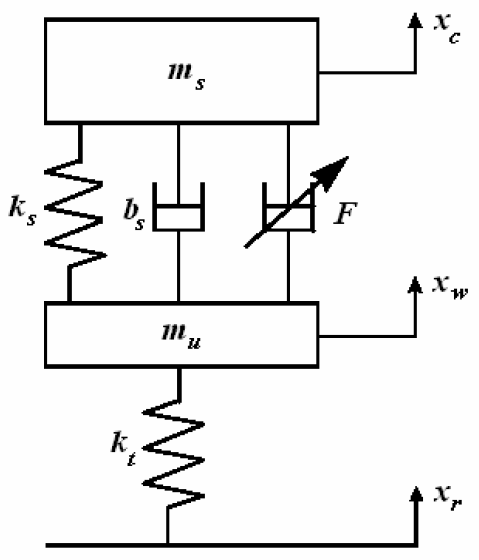
\includegraphics[width=5cm]{img/massa_mola_nao_linear_controlavel.png}
            \caption{Modelo de suspensão para um quarto de carro.} 
            \label{fig:massa_mola_nao_linear_controlavel}
        \end{centering}
    \end{figure}
    \FloatBarrier
    Na figura \ref{fig:massa_mola_nao_linear_controlavel} temos que $m_s$ representa a massa suspensa que consiste em um quarto da massa total da carroceria do veiculo em \emph{kg}, $m_u$ representa a massa não suspensa ou a massa do eixo e da roda em \emph{kg}, $b_s$ representa o o coeficiente de amortecimento do amortecedor passivo em \emph{Ns/m}, $k_s$ representa o coeficiente de elasticidade do feixe de molas da suspensão, segundo a lei de hooke, em \emph{N/m}, $k_t$ representa o coeficiente de elasticidade do pneu, segundo a lei de hooke, em \emph{N/m}, $x_r$ representa o deslocamento vertical da pista, onde o sufixo $r$ significa \emph{road}, em \emph{m}, $x_w$ representa o deslocamento vertical da roda, onde o sufixo $w$ significa \emph{wheel}, em \emph{m} e $x_c$ representa o deslocamento vertical da carroceria, onde o sufixo $c$ significa \emph{carr}, em \emph{m}. Na mesma figura o simbolo $F$ representa a atuação de um dispositivo amortecedor com características dinâmicas, seja ele ativo ou semi-ativo, em \emph{N}.
    
    O diagrama de corpo livre do sistema pode ser construído tomando-se como referencia a coordenada da posição do eixo da roda $x_w$ como pode ser observado nas figuras \ref{fig:corpo_livre_ms} e \ref{fig:corpo_livre_mu} a seguir:
    \FloatBarrier
    \begin{figure}[htbp]
        \begin{centering}
            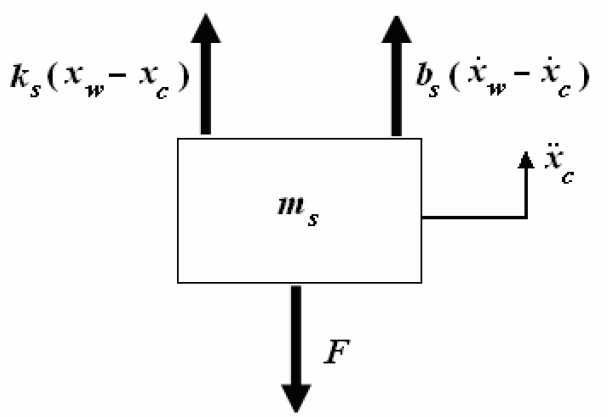
\includegraphics[width=5cm]{img/corpo_livre_ms.png}
            \caption{Diagrama de corpo livre para a massa $m_s$.} 
            \label{fig:corpo_livre_ms}
        \end{centering}
    \end{figure}
    \FloatBarrier
    \begin{figure}[htbp]
        \begin{centering}
            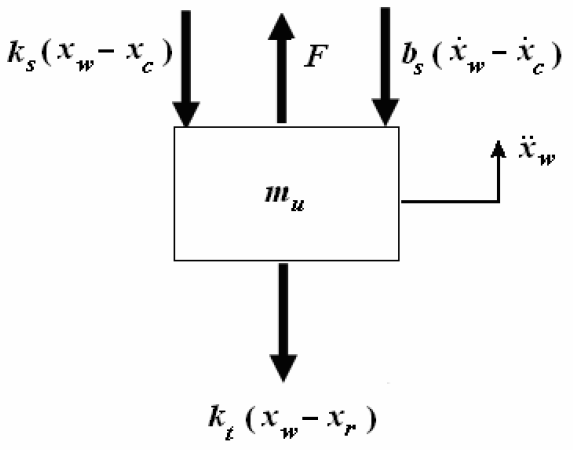
\includegraphics[width=5cm]{img/corpo_livre_mu.png}
            \caption{Diagrama de corpo livre para a massa $m_u$.} 
            \label{fig:corpo_livre_mu}
        \end{centering}
    \end{figure}
    \FloatBarrier
    
    Aplicando a segunda lei de Newton $\sum{F}=m.a$, a cada uma das massas separadamente, o sistema para o modelo de um quarto de carro da figura \ref{fig:massa_mola_nao_linear_controlavel} pode ser representado pela seguinte equação:
    
    \begin{equation} \label{eq:massa_mola_linear}
    \begin{split}
        m_{s} \ddot{x}_{c} =&  b_{s}(\dot{x}_{w}-\dot{x}_{c}) + k_{s}(x_{w}-x_{c}) - F\ \\
        m_{u} \ddot{x}_{w} =& -b_{s}(\dot{x}_{w}-\dot{x}_{c}) - k_{s}(x_{w}-x_{c})  k_{t}(x_{w}-x_{r}) + F
    \end{split}
    \end{equation}
    
    A equação \ref{eq:massa_mola_linear} representa o modelo do sistema na forma linear. Porém a mola $k_s$, o amortecedor $b_s$ e o amortecedor dinâmico ativo podem ser modelados através de modelos lineares ou modelos não lineares. \\
    Uma mola linear obedece a lei de Hooke apresentando uma deformação proporcional ao carregamento. Em uma mola não linear o coeficiente de elasticidade da mola cresce exponencialmente conforme se afasta do ponto de equilíbrio estático.
    Para um modelo de mola não linear, podemos utilizar seguinte expressão para a força da mola $ k_{s}(x_{w}-x_{c})$:
    
    \begin{equation} \label{eq:mola_nao_linear}
        k_{s}(x_{w}-x_{c}) = k^{l}_{s}(x_{w}-x_{c})+k^{nl}_{s}(x_{w}-x_{c})^{3}
    \end{equation}
        
    Na equação \ref{eq:mola_nao_linear} o coeficiente $k^{l}_{s}$ representa o coeficiente de elasticidade do termo da faixa de operação linear e o coeficiente $k^{nl}_{s}$] representa o coeficiente de elasticidade do termo da faixa de operação não linear do feixe de molas em uma situação real.\\
    A não linearidade do amortecedor permite que pequenos movimentos causados pelo perfil da estrada gerem apenas um pequeno impacto na carroceria além de apresentar saturação e histerese. Para um modelo de amortecedor não linear, podemos utilizar a seguinte expressão:
 
    \begin{equation} \label{eq:amortecedor_nao_linear}
        \begin{aligned}
        b_{s}(\dot{x}_{w}-\dot{x}_{c}) =\ \ &b^{l}_{s}(\dot{x}_{w}-\dot{x}_{c}) - b^{y}_{s}\mid\dot{x}_{w}-\dot{x}_{c}\mid \\
        + &b^{nl}_{s}\sqrt{\mid\dot{x}_{w}-\dot{x}_{c}\mid}sgn(\dot{x}_{w}-\dot{x}_{c})  
        \end{aligned}
    \end{equation}
    
    Na equação \ref{eq:amortecedor_nao_linear} o coeficiente $b^{l}_{s}$ representa o coeficiente de amortecimento do termo da faixa de operação linear, o coeficiente $b^{l}_{s}$ representa o coeficiente de amortecimento do termo da faixa de operação não linear e o coeficiente $b^{y}_{s}$ representa a característica de comportamento assimétrico do amortecedor.
    
    Substituindo as equações \ref{eq:mola_nao_linear} e \ref{eq:amortecedor_nao_linear} em \ref{eq:massa_mola_linear} obtemos as seguintes equações diferenciais dinâmicas de segunda ordem que representam a dinâmica de um sistema de suspensão ativa não linear:
    
    \begin{equation} \label{eq:massa_mola_nao_linear}
        \begin{aligned}
         m_{s} \ddot{x}_{c} =\ \ &k^{l}_{s}(x_{w}-x_{c})+k^{nl}_{s}(x_{w}-x_{c})^{3}+b^{l}_{s}(\dot{x}_{w}-\dot{x}_{c})\\
                            -&b^{y}_{s}\mid\dot{x}_{w}-\dot{x}_{c}\mid+b^{nl}_{s}\sqrt{\mid\dot{x}_{w}-\dot{x}_{c}\mid}sgn(\dot{x}_{w}-\dot{x}_{c})\\ 
                            -&F\\
         m_{u} \ddot{x}_{w} = -&k^{l}_{s}(x_{w}-x_{c})-k^{nl}_{s}(x_{w}-x_{c})^{3}-b^{l}_{s}(\dot{x}_{w}-\dot{x}_{c})\\  
                            +&b^{y}_{s}\mid\dot{x}_{w}-\dot{x}_{c}\mid-b^{nl}_{s}\sqrt{\mid\dot{x}_{w}-\dot{x}_{c}\mid}sgn(\dot{x}_{w}-\dot{x}_{c})\\
                            -&k_{t}(x_{w}-x_{r})+F\\
        \end{aligned}
    \end{equation}
    \subsection{Modelo Linearizado de um sistema de suspensão semi-ativa, não linear, de um quarto de veículo, com dois graus de liberdade }
    Realizando a distributiva no sistema descrito em \ref{eq:massa_mola_nao_linear} e Propondo as seguintes substituições para as variáveis de estado das equações e reorganizando os termos, obtemos: 
    \begin{equation*}
        \begin{split}
            x_{1}=&x_{c};\ \ \\
            x_{2}=&\dot{x}_{c};\ \ \\
            x_{3}=&x_{w};\ \ \\
            x_{4}=&\dot{x}_{w};\ \ \\
        \end{split}
        \begin{split}
            \dot{x}_{1}=&\dot{x}_{c};\ \ \\
            \dot{x}_{2}=&\ddot{x}_{c};\ \ \\
            \dot{x}_{3}=&\dot{x}_{w};\ \ \\
            \dot{x}_{4}=&\ddot{x}_{w};\ \ \\
        \end{split}
        \begin{split}
            w=&x_{r};\ \ \\
            u=&F;\ \ \\
        \end{split} 
    \end{equation*}
    \begin{equation} \label{eq:massa_mola_nao_linear}
        \begin{aligned}
        \dot{x}_{1}=&\ \ \ \ x_{2}\\
        \dot{x}_{2}=&-\frac{k^l_s}{m_s}x_1-\frac{b^l_s}{m_s}x_2+\frac{k^l_s}{m_s}x_3+\frac{b^l_s}{m_s}x_4-\frac{k^{nl}_s}{m_s}(x_3-x_1)^3\\
                    &+\frac{b^y_s}{m_s}\mid x_4-x_2\mid+\frac{b^{nl}_s}{m_s}\sqrt{\mid x_4-x_2\mid}sgn(x_4-x_2)\\
                    &-\frac{1}{m_s}u\\
        \dot{x}_{3}=&\ \ \ \ x_{4}\\
        \dot{x}_{4}=&\ \ \ \ \frac{k^l_s}{m_u}x_1+\frac{b^l_s}{m_u}x_2-\frac{k^l_s}{m_u}x_3-\frac{b^l_s}{m_u}x_4+\frac{k^{nl}_s}{m_u}(x_3-x_1)^3\\
                    &-\frac{b^y_s}{m_u}\mid x_4-x_2\mid-\frac{b^{nl}_s}{m_u}\sqrt{\mid x_4-x_2\mid}sgn(x_4-x_2)\\
                    &+\frac{k_t}{m_u}w+\frac{1}{m_u}u\\
        \end{aligned}
    \end{equation}
    
    \subsection{Linearização do modelo em espaço de estados}
    
    Um sistema dinâmico descrito por meio de equações diferenciais não lineares pode ser linearizado na proximidade de um ponto de equilíbrio através do método da expansão em série de Taylor truncada no seu segundo termo como exibido na equação a seguir:
    
    \begin{equation}
        P(x) = f(\alpha) + \dfrac{\mathrm{d}f(\alpha)}{\mathrm{d}x}*\frac{(x-\alpha)^{-1}}{1!}    
    \end{equation}
    
    Onde $\alpha$ é um ponto de equilíbrio da equação $P(x)$.  
    Para um sistema com múltiplas variáveis de estado, calcula-se a Jacobiana do sistema para realizar a linearização em torno do ponto de operação escolhido.  
    
    \begin{equation} \label{eq:Jacobian_A}
    \mathbf{J_A}(x_1,x_2,\dots,x_n) =
        \begin{bmatrix}
            \frac{\partial x_1}{\partial x_1} & 
            \frac{\partial x_1}{\partial x_2} & 
            \dots &
            \frac{\partial x_1}{\partial x_n} &\\[1ex]
            \frac{\partial x_2}{\partial x_1} & 
            \frac{\partial x_2}{\partial x_2} & 
            \dots &
            \frac{\partial x_2}{\partial x_n} &\\[1ex]
            \vdots & 
            \vdots & 
            \ddots &
            \vdots &\\[1ex]
            \frac{\partial x_n}{\partial x_1} & 
            \frac{\partial x_n}{\partial x_2} & 
            \dots &
            \frac{\partial x_n}{\partial x_n} &\\[1ex]
    \end{bmatrix}
    \end{equation}
    
    \begin{equation} \label{eq:eval_A}
        \mathbf{A=J_A} \Bigr\rvert_{(x_1=\alpha_1;x_2=\alpha_2;\dots;x_n=\alpha_n)} \\
    \end{equation}
    
    \begin{equation} \label{eq:Jacobian_B}
    \mathbf{J_B}(u_1,u_2,\dots,u_m) =
        \begin{bmatrix}
            \frac{\partial u_1}{\partial u_1} & 
            \frac{\partial u_1}{\partial u_2} & 
            \dots &
            \frac{\partial u_1}{\partial u_m} &\\[1ex]
            \frac{\partial u_2}{\partial u_1} & 
            \frac{\partial u_2}{\partial u_2} & 
            \dots &
            \frac{\partial u_2}{\partial u_m} &\\[1ex]
            \vdots & 
            \vdots & 
            \ddots &
            \vdots &\\[1ex]
            \frac{\partial u_n}{\partial u_1} & 
            \frac{\partial u_n}{\partial u_2} & 
            \dots &
            \frac{\partial u_m}{\partial u_m} &\\[1ex]
    \end{bmatrix}
    \end{equation}
    
    \begin{equation} \label{eq:eval_B}
        \mathbf{B=J_B} \Bigr\rvert_{(u_1=\beta_1;u_2=\beta_2;\dots;u_m=\beta_m)} \\
    \end{equation}
    
    \begin{equation} \label{eq:sis_lenearizado}
        Y(x,u) = A*x + B*u
    \end{equation}
    
     Onde:
     \begin{itemize}
        \item $x=[x_1,x_2,\dots,x_n]$ o vetor de estados do sistema
        \item $u=[u_1,u_2,\dots,u_m]$ o vetor das entradas do sistema
        \item $\alpha=[\alpha_1,\alpha_2,\dots,\alpha_n]$ um vetor solução para os pontos de equilíbrio dos estados do sistema.
        \item $\beta=[\beta_1,\beta_2,\dots,\beta_m]$ um vetor solução para os pontos de equilíbrio das entradas do sistema.
        \item $Y(x,u)$ equação do sistema linearizado ao redor do ponto de equilíbrio $\alpha$.
     \end{itemize}
     
    
    \subsection{Especificações da Resposta Transitória para Sistemas Subamortecidos}
    As características de um sistema de controle são geralmente especificadas em termos da resposta transitória para uma entrada em degrau. Para sistemas LIT, quando a resposta ao degrau é conhecida, pode-se calcular a resposta a qualquer tipo de entrada e Costuma-se utilizar condição inicial de sistema em repouso. As seguintes especificações são as mais utilizadas:
    \begin{itemize}
        \item  Tempo de atraso - $t_d$: tempo necessário para que a resposta alcance metade do seu valor final pela primeira vez.
        \item  Tempo de subida - $t_r$: tempo requerido para que a resposta passe de 10\% a 90\%, ou de 5\% a 95\%, ou de 0\% a 100\% do valor final. Para sistemas de 2ª ordem subamortecido, utiliza-se 0\% a 100\% do valor final. Para sistemas superamortecidos, geralmente considera-se de 10\% a 90\%.
        \begin{equation} \label{eq:tr}
            t_r = \frac{\pi-\theta}{\omega_d}
        \end{equation} 
        \item Tempo de pico - $t_p$: tempo para que a resposta atinja o primeiro pico de sobressinal.
        \begin{equation} \label{eq:tp}
            t_p = \frac{\pi}{\omega_d}
        \end{equation}
        \item Máximo Overshoot $MO$: valor máximo de pico da curva de resposta, medido a partir da unidade. Se o valor da resposta em regime diferir da unidade, utiliza-se a porcentagem máxima de sobressinal (ou ultrapassagem percentual, U.P.):
        \begin{equation} \label{eq:MO}
        \begin{split}
            M_O=\exp{(\frac{-\xi.\pi}{\sqrt(1-\xi^2)})}\\
            \xi=-\frac{ln\left( M_O \right)}{\sqrt{\pi^2+ln^2(M_O)}}    
        \end{split}
        \end{equation}
        \item Tempo de acomodação ou assentamento - $t_s$: tempo necessário para que a resposta permaneça com valores no interior de uma certa faixa (usualmente $\pm2\%$ ou $\pm5\%$) em torno do valor final.
        \begin{equation} \label{eq:Ts2}
        \begin{split}
            T_{S_{2\%}}=-\frac{ln\left( 0.02*\sqrt{1-\xi} \right)}{\omega_n*\xi}\\
            \omega_n=-\frac{ln\left( 0.02*\sqrt{1-\xi} \right)}{T_{S_{2\%}}*\xi}  
        \end{split}
        \end{equation}
    \end{itemize}

    Dado que:
    \begin{equation} \label{eq:eign}
            \lambda = \sigma \pm \omega_d.i
    \end{equation}
    \begin{equation} \label{eq:xi}
        \xi=\frac{\sigma}{|\omega_n|}
    \end{equation}
    \begin{equation} \label{eq:theta}
            \xi=\cos{(\theta)}
    \end{equation}
    \begin{equation} \label{eq:wd}
            \omega_d=\omega_n\sqrt{1-\xi^2}
    \end{equation}
    
    \subsection{Alocação de polos pela fórmula de Lyapunov} \label{sc:lyapunov}
    
    Considere o par $(A,b)$ controlável, com $A \in \mathbb{R}^{n*n}$ e $b \in \mathbb{R}^{n*1}$. Dada uma matriz $F \in \mathbb{R}^{n*n}$ arbitrária com os autovalores desejados para a resposta do sistema dinâmico em malha fechada, é possível encontrar um vetor de ganhos de realimentação $K\in \mathbb{R}^{1*n}$ tal que $eig(A-b*K)=eig(F)$ desde que $eig(A)\neq eig(F)$ através dos seguintes passos:
    
    \begin{enumerate}
        \item Escolha uma matriz $F \in \mathbb{R}^{n*n}$ com os autovalores desejados.
        \item Escolha um $\bar{k}$ arbitrário tal que $(F,\bar{k})$ seja observável.
        \item {Obtenha a única solução $T$ da equação de Lyapunov
        \begin{equation} \label{eq:lyapunov}
            AT-TF=b\bar{k}
        \end{equation}}
        \item {Compute o ganho de realimentação:
        \begin{equation} \label{eq:ganho}
            K=\bar{k}T^{-1}
        \end{equation}}
    \end{enumerate}
    
    \section{Metodologia}
    \subsection{Linearização do modelo em espaço de estados}
        
    O sistema proposto possui um ponto de equilíbrio na origem do sistema:
    \begin{equation*}
        \begin{split}
        x_1=\ \ &0\\
        x_2=\ \ &0\\
        x_3=\ \ &0\\
        x_4=\ \ &0\\
        \end{split}
    \end{equation*}
    Para realizar a linearização em torno do ponto de operação escolhido calcula-se a Jacobiana do sistema de equações dinâmicas não lineares descrito em \ref{eq:massa_mola_nao_linear} através das equações \ref{eq:Jacobian_A} e \ref{eq:Jacobian_B}. Em seguida, calculou-se o valor da Jacobiana no valor especifico do ponto de equilibro, conforme as equações \ref{eq:eval_A} e \ref{eq:eval_B}, obtemos as matrizes $A$ e $B$ do sistema linearizado exibidas a seguir:
 
    \begin{equation*} 
    \begin{split}
        \mathbf{A} =
        \begin{bmatrix}
            0 & 1 & 0 & 0 & \\
            -\frac{k_{s}^{l}}{m_s}&-\frac{b_{s}^{l}}{m_s}&\frac{k_{s}^{l}}{m_s}&\frac{b_{s}^{l}}{m_s} &\\ \\
            0 & 0 & 0 & 1 & \\
            \frac{k_{s}^{l}}{m_u}&\frac{b_{s}^{l}}{m_u}&-\frac{(k_{s}^{l}+k_t)}{m_u}&-\frac{b_{s}^{l}}{m_u} &\\
        \end{bmatrix};
    \end{split}
    \begin{split}
       \mathbf{x} = 
        \begin{bmatrix}
             x_1 &\\
             x_2 &\\
             x_3 &\\
             x_4 &\\
        \end{bmatrix}; 
    \end{split}
    \end{equation*}
    
    \begin{equation} 
    \begin{split}
        \mathbf{B} = 
        \begin{bmatrix}
            0 & 0 & \\
            0 & -\frac{1}{m_s}&\\ \\
            0 & 0 & \\
            \frac{k_t}{m_u}&\frac{1}{m_u} \\
        \end{bmatrix}
    \end{split}
    \end{equation}
    
    É esperado que o  sistema linearizado se aproxime do sistema não linear enquanto opere na vizinhança do ponto de equilíbrio utilizado para linearização. Que para este caso é a origem do sistema formado pelas variáveis de estado.
    \subsection{Simulação da resposta temporal do modelo linearizado em malha aberta}
    Abaixo seguem figuras que ilustram a simulação temporal do sistema não linear e linearizado para 3 diferentes condições iniciais a parâmetros do sistema dados a seguir: 
    
    \begin{equation*} 
    \begin{split}
        \begin{bmatrix}
            x_c & \dot{x}_c & x_w & \dot{x}_w & \\
        \end{bmatrix}=
    \end{split}
    \begin{split}
        \begin{bmatrix}
            -0.01& -0.01& 0& 0& \\
             -0.1&  -0.1& 0& 0& \\
             -0.5&  -0.5& 0& 0&\\
        \end{bmatrix}
    \end{split}
    \end{equation*}
    
   \begin{equation} \label{eq:parametros}
        \begin{split} 
        m_s =   & 290     [kg]\\
        m_u =   & 40      [kg]\\
        b^{l}_s =  & 700  [Ns.m^{-1}]\\
        b^{nl}_s =  & 200      [Ns.m^{-1}]\\
        b^{y}_s=  & 400      [Ns.m^{-1}]\\
        k^{l}_s =  & 235.10^2 [N.m^{-1}]\\
        k^{nl}_s = & 235.10^4 [N.m^{-1}]\\
        k_t =  & 190.10^3 [N.m^{-1}]\\
        \end{split}
    \end{equation}

    \FloatBarrier
    \begin{figure}[htbp]
        \begin{centering}
            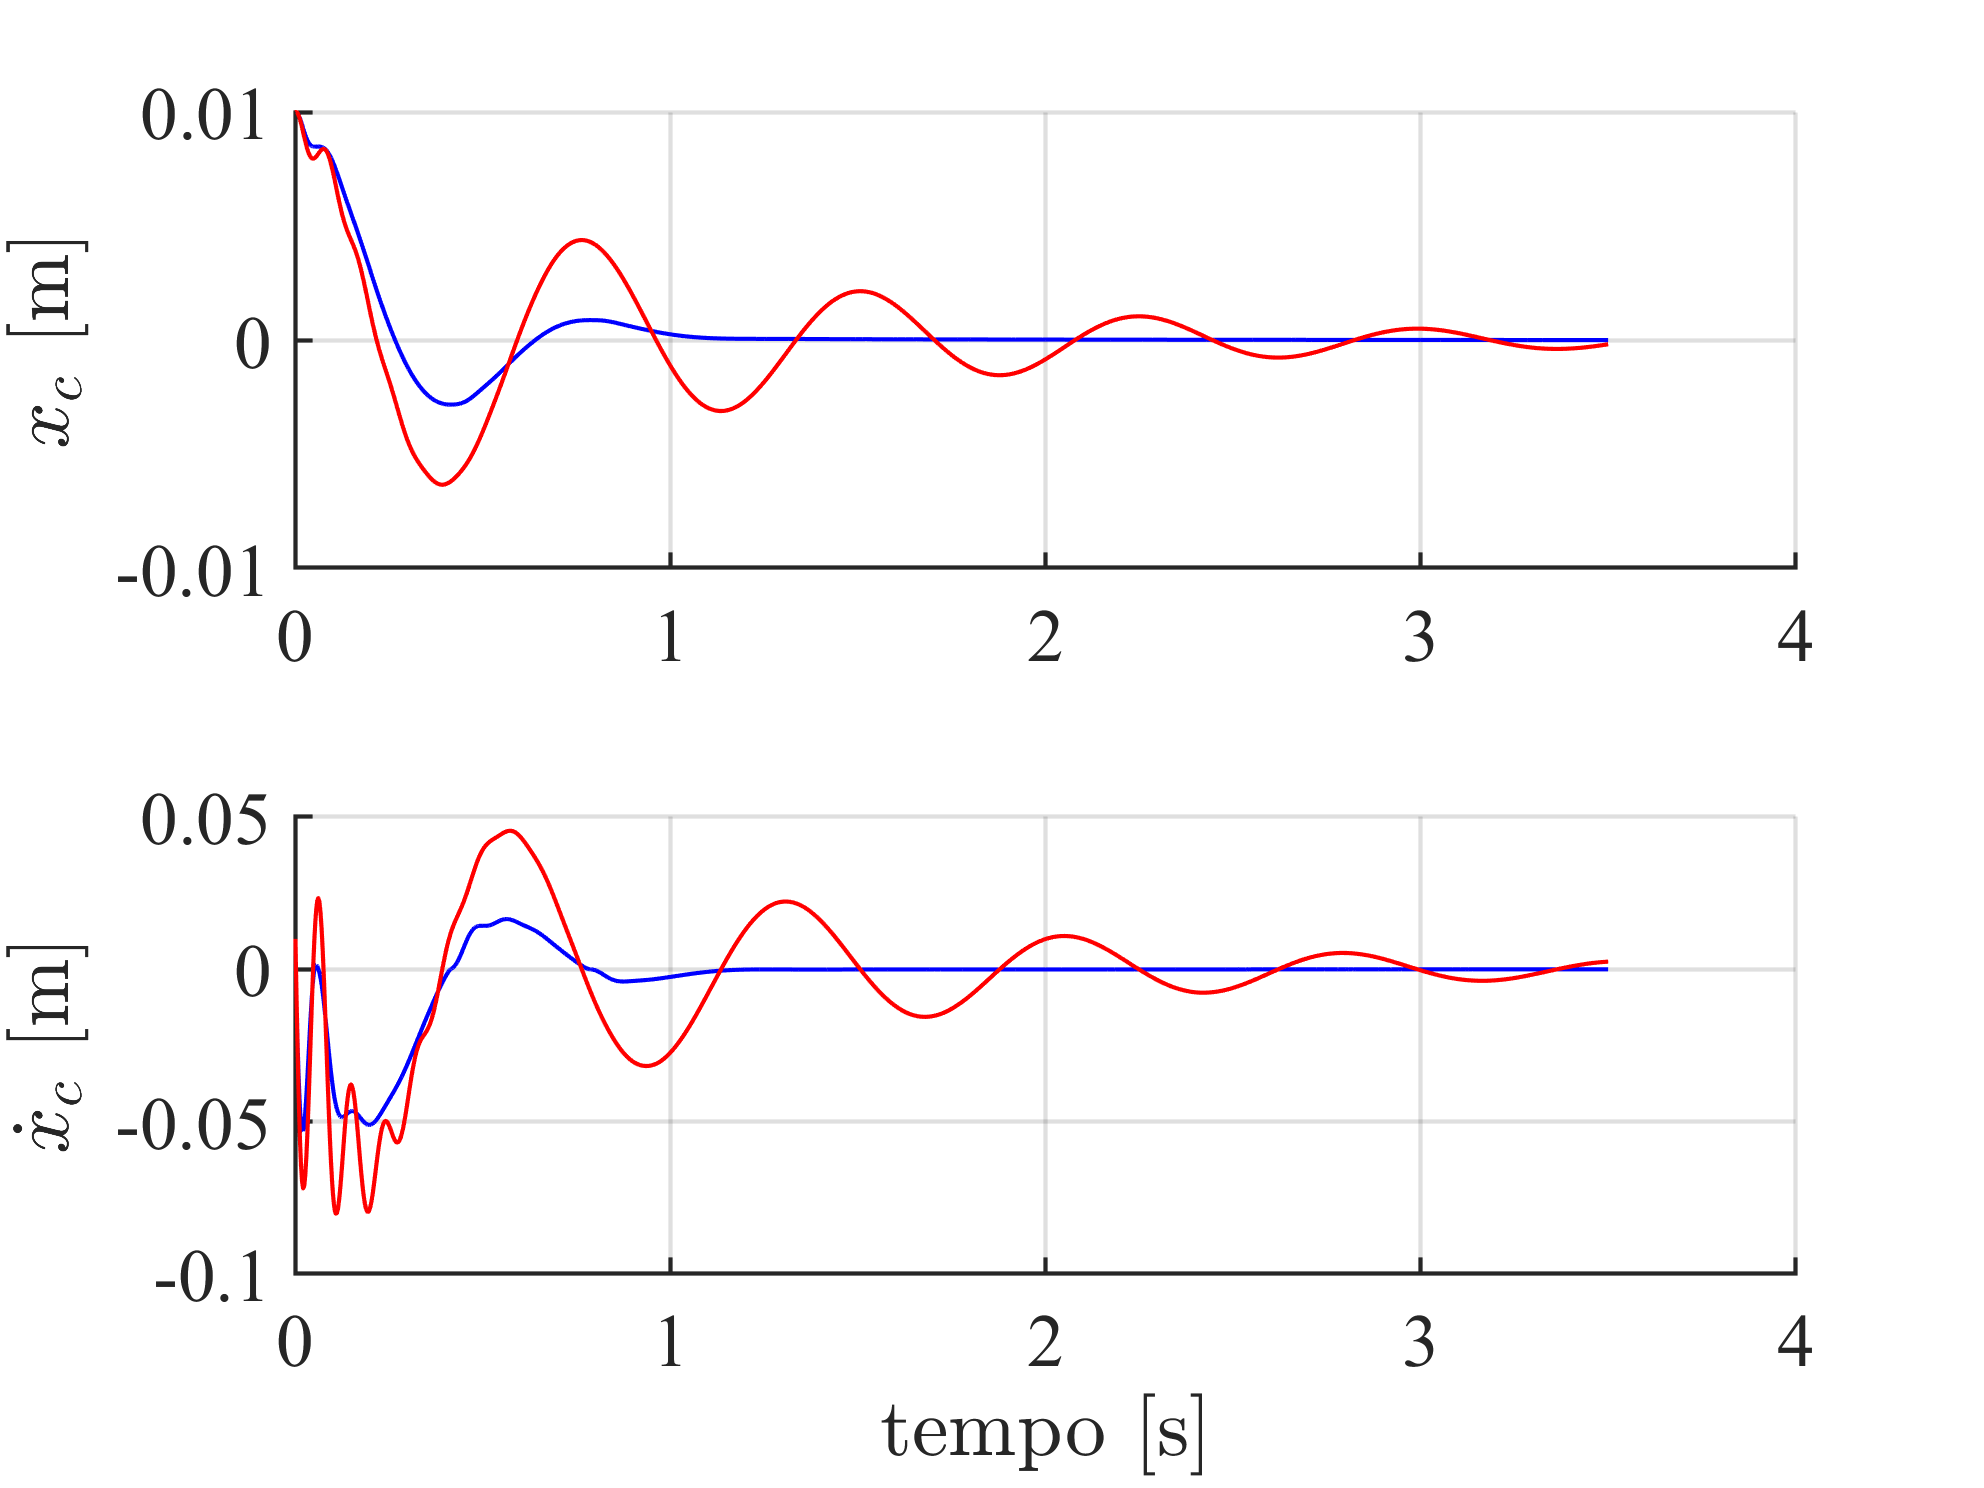
\includegraphics[width=6cm]{img/sim_temp_xc_n001_dxc_n001.png}
            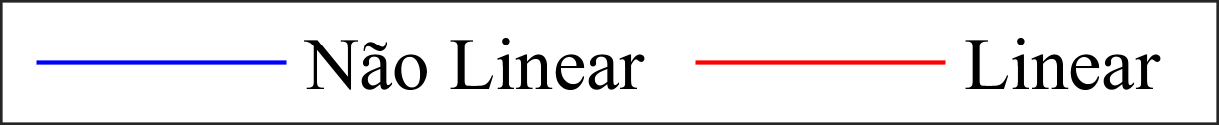
\includegraphics[width=5cm]{img/sim_temp_Leg.png}
            \caption{Simulação temporal do sistema para as condições iniciais:  $[x_c, \dot{x}_c, x_w, \dot{x}_w]=[-0.01,-0.01,0,0]$}
            \label{fig:sim_temp_xc_n01_dxc_n01}
        \end{centering}
    \end{figure}
    \FloatBarrier
    
    \FloatBarrier
    \begin{figure}[htbp]
        \begin{centering}
            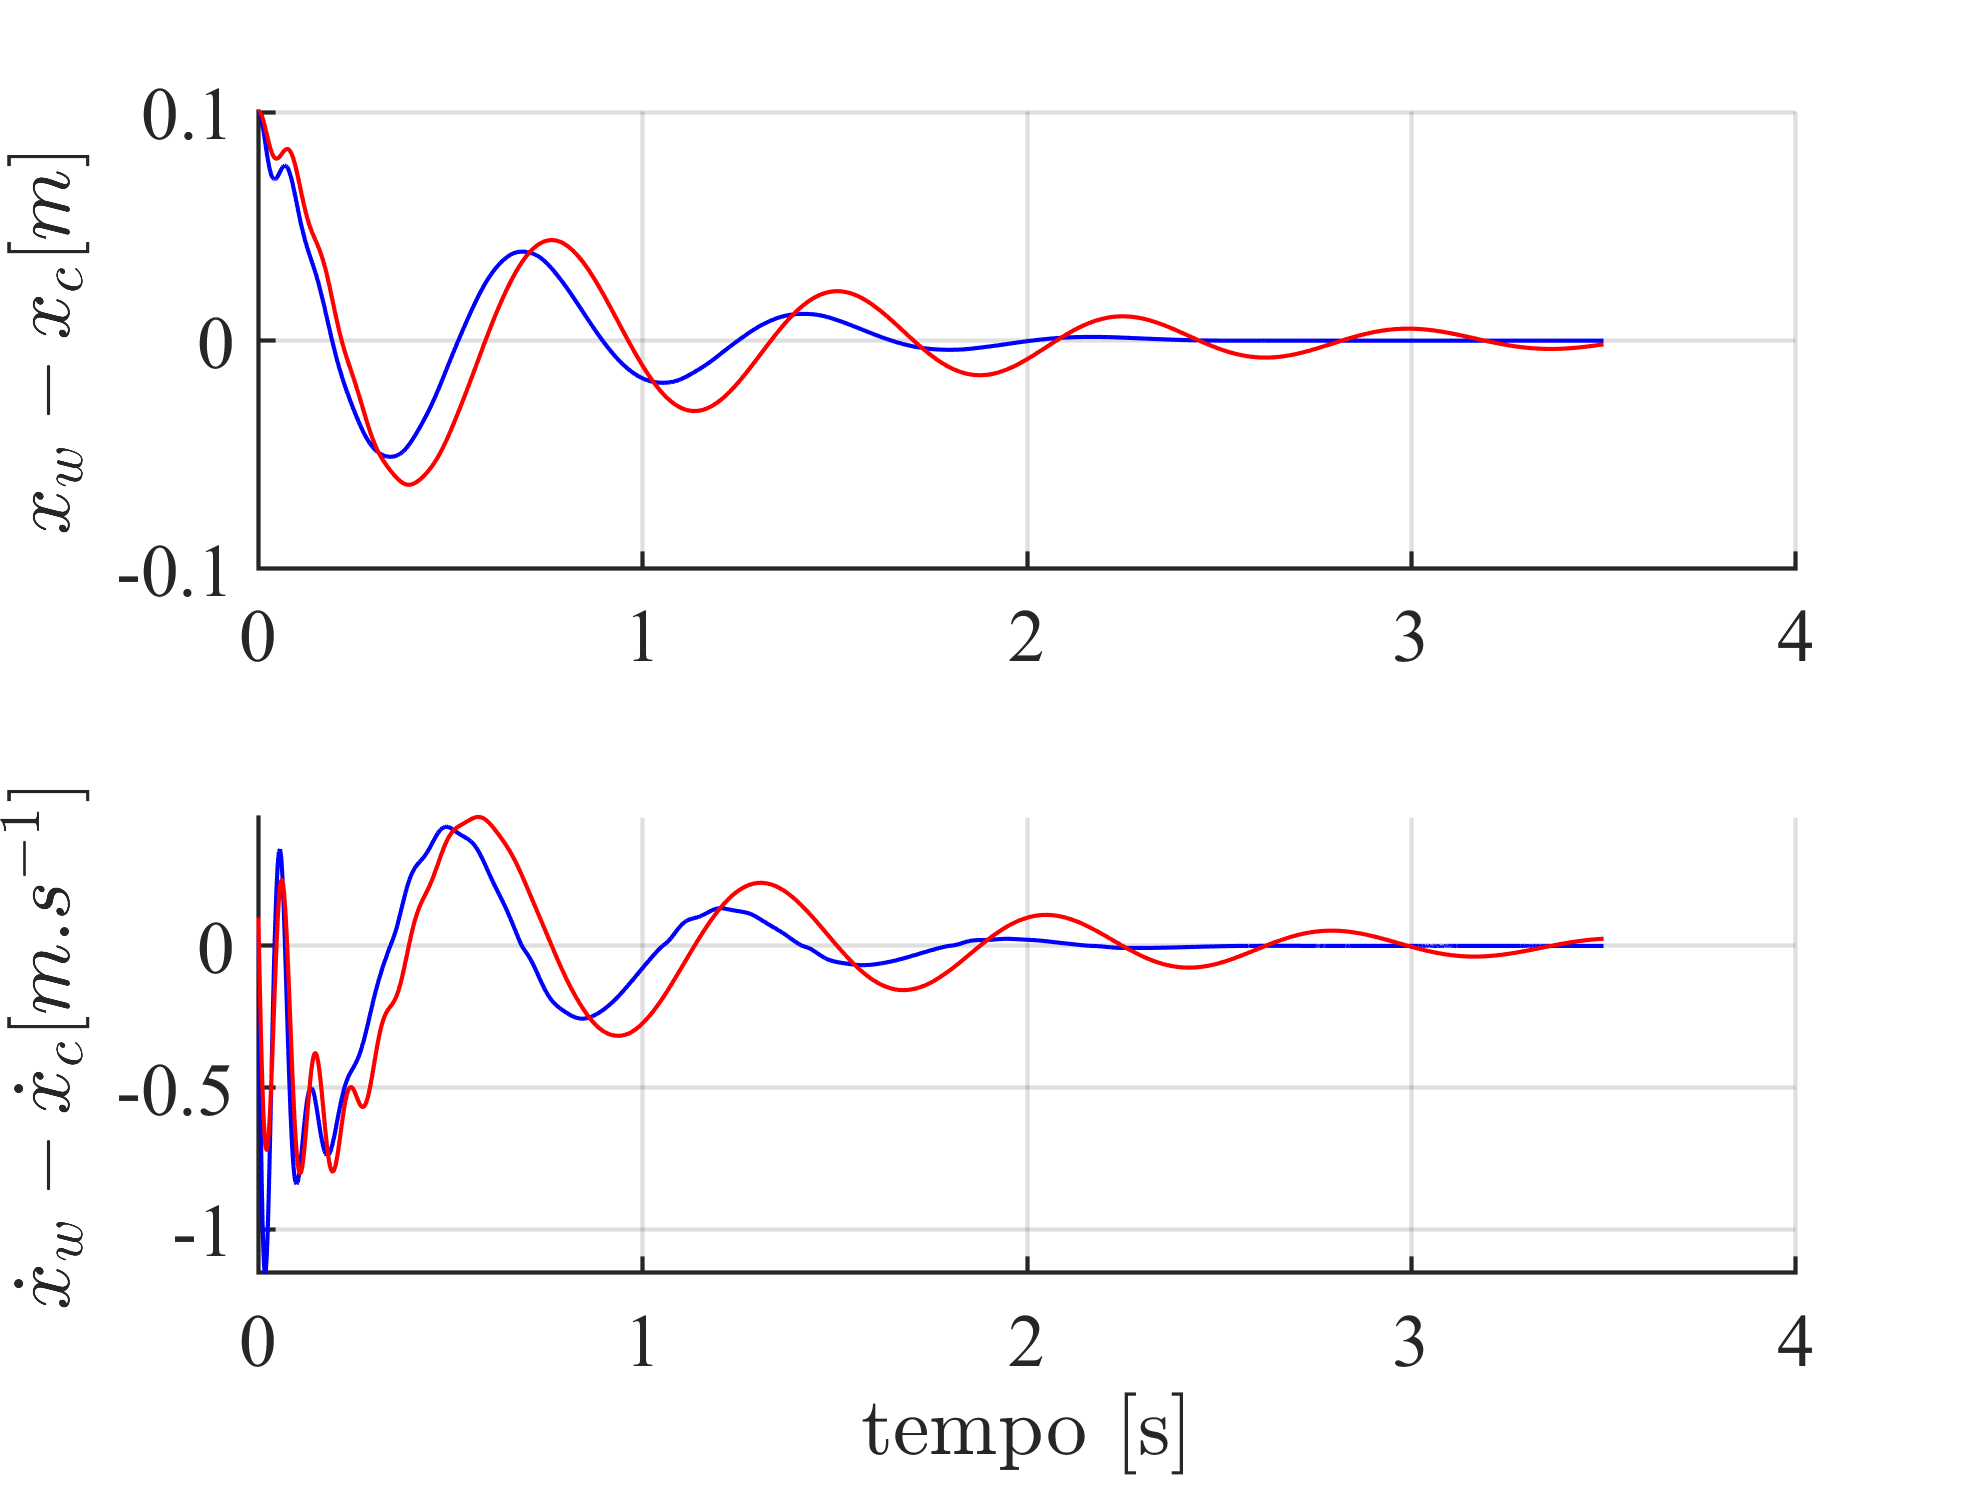
\includegraphics[width=6cm]{img/sim_temp_xc_n01_dxc_n01.png}
            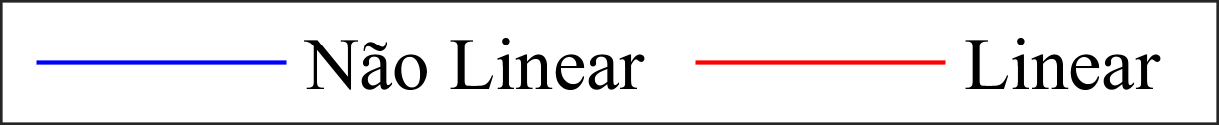
\includegraphics[width=5cm]{img/sim_temp_Leg.png}
            \caption{Simulação temporal do sistema para as condições iniciais:  $[x_c, \dot{x}_c, x_w, \dot{x}_w]=[-0.1,-0.1,0,0]$}
            \label{fig:sim_temp_xc_n01_dxc_n01}
        \end{centering}
    \end{figure}
    \FloatBarrier
    
    \FloatBarrier
    \begin{figure}[htbp]
        \begin{centering}
            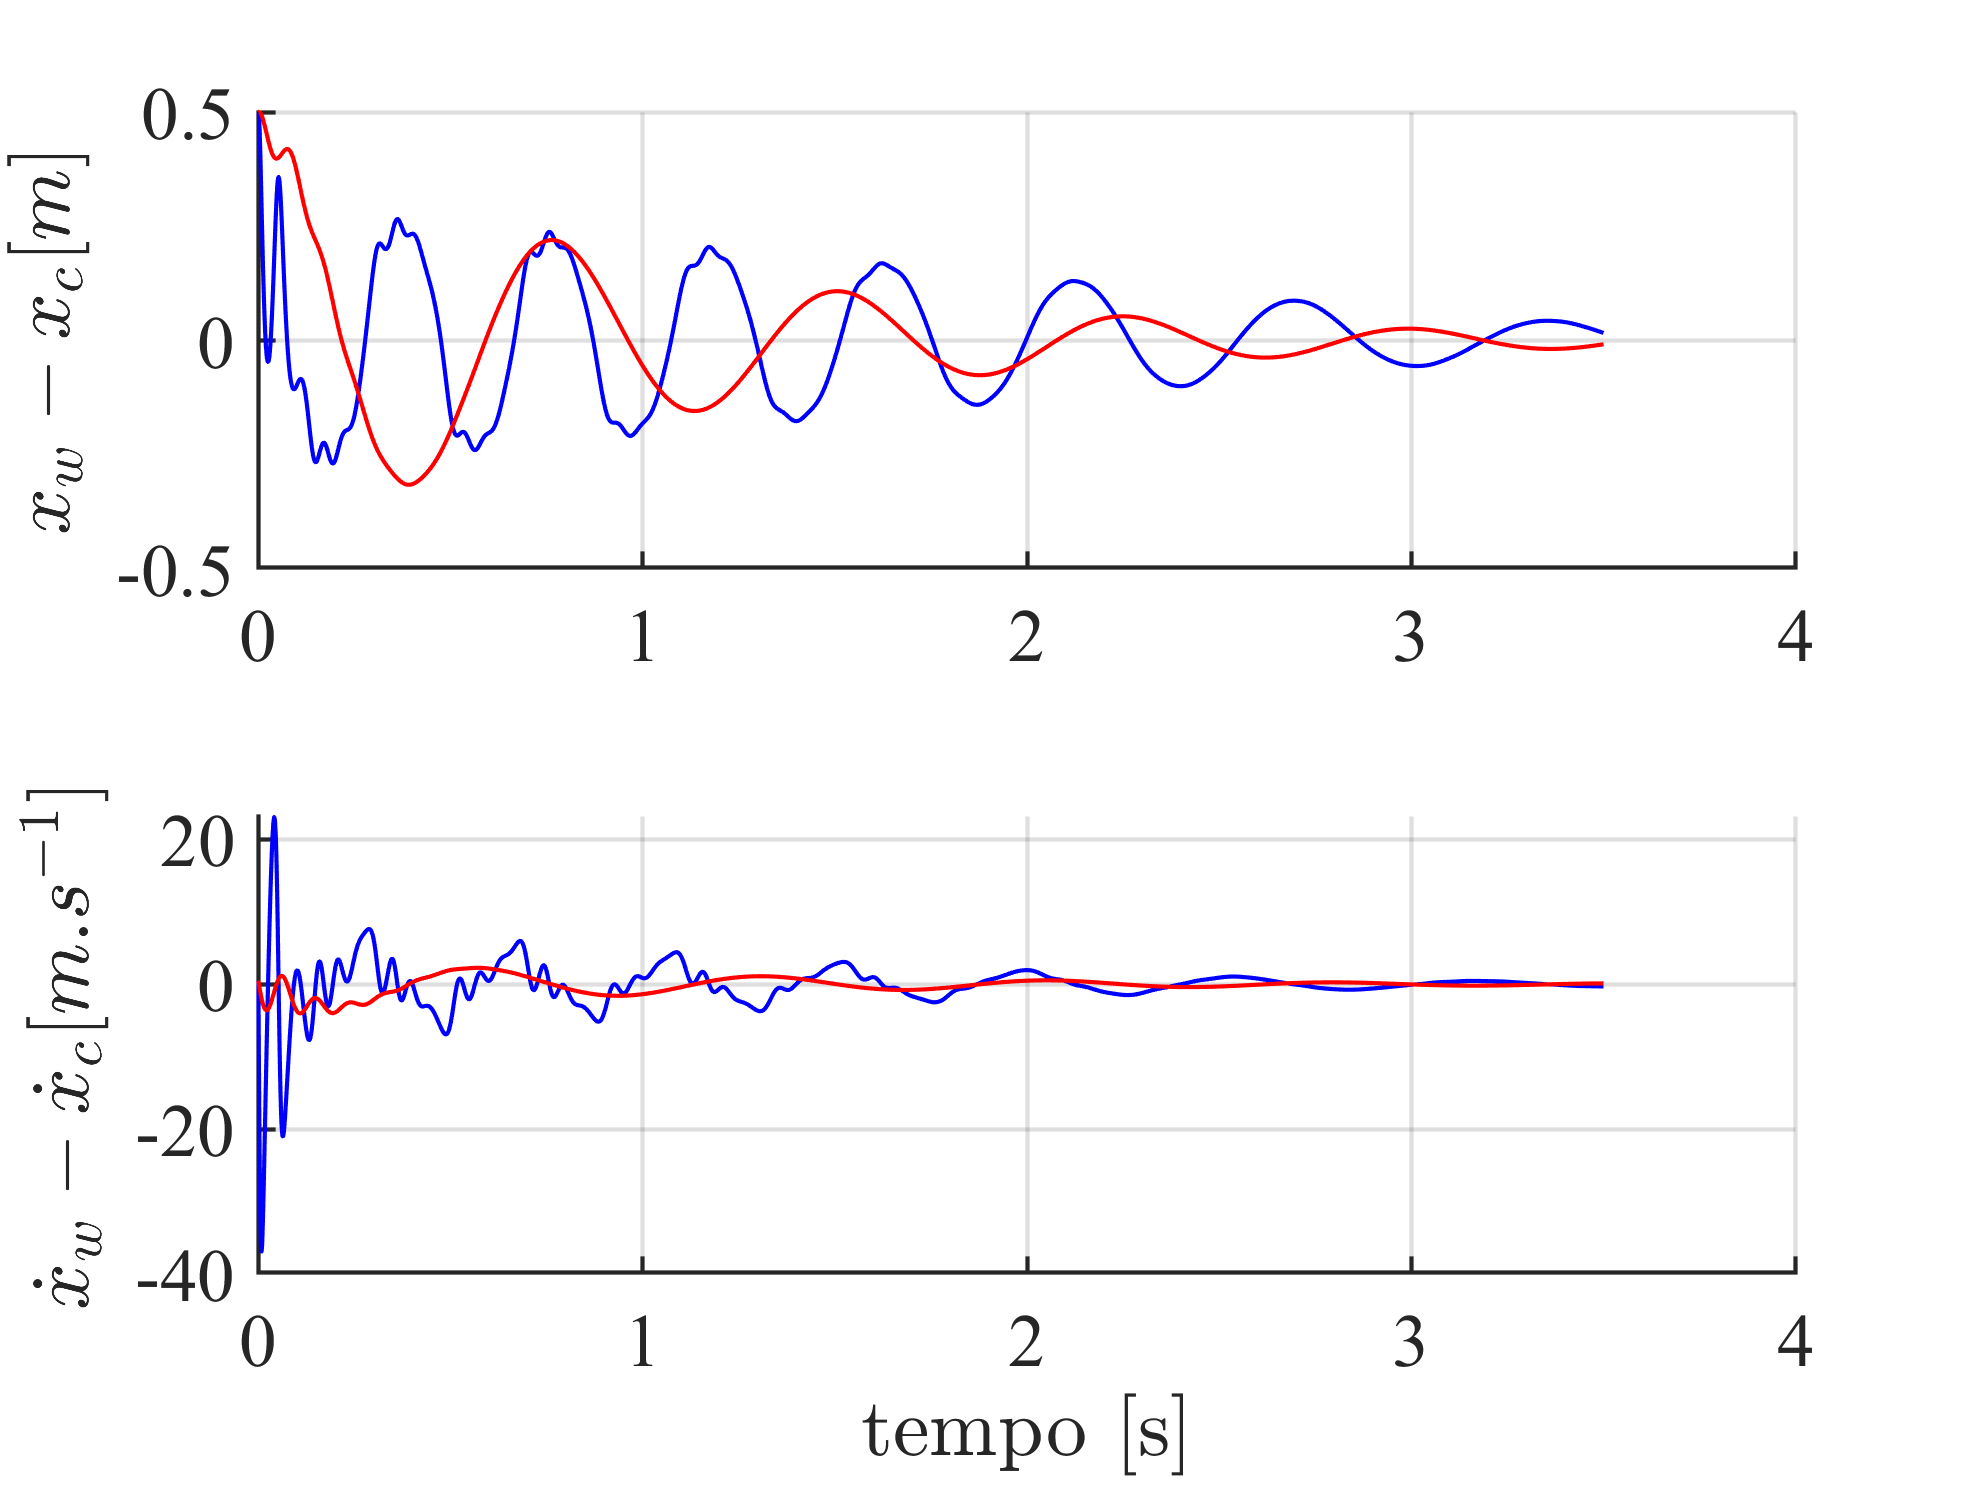
\includegraphics[width=6cm]{img/sim_temp_xc_n05_dxc_n05.png}
            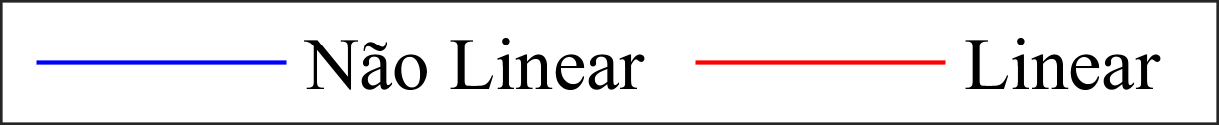
\includegraphics[width=5cm]{img/sim_temp_Leg.png}
            \caption{Simulação temporal do sistema para as condições iniciais:  $[x_c, \dot{x}_c, x_w, \dot{x}_w]=[-0.5,-0.5,0,0]$}
            \label{fig:sim_temp_xc_n01_dxc_n01}
        \end{centering}
    \end{figure}
    \FloatBarrier
    
    Pode-se observar a diferença dramática entre as simulações temporais dos sistemas para a condição inicial $[x_c, \dot{x}_c, x_w, \dot{x}_w]=[-0.5,-0.5,0,0]$ devido a esta ser a que mais se afasta do ponto de equilíbrio utilizado para linearização do sistema
    
    \subsection{Análise da estabilidade do sistema em malha aberta}
    
    Para o sistema linearizado com parâmetros dados pela equação \ref{eq:parametros} obtemos os seguinte conjunto de autovalores para a Matriz $A$ do sistema:
    
    \begin{equation}
    \begin{split}
    \mathbf{A} =
        \begin{bmatrix}
               0&      1&        0&     0&\\ \\
               -\frac{2350}{29}& -\frac{70}{9}&  \frac{2350}{29}& \frac{70}{29}&\\ \\
               0&      0&        0&     1&\\ \\
                \frac{1175}{2}&   \frac{35}{2}& -\frac{10675}{2}& -\frac{35}{2}&\\ 
        \end{bmatrix}; \ \
    \end{split}
   \begin{split}
   \mathbf{B} =
        \begin{bmatrix}
               0&      0&\\ \\
               0& -\frac{1}{290}&\\ \\
               0&      0&\\ \\
            4750&   \frac{1}{40}&\\
        \end{bmatrix}
   \end{split}     
    \end{equation}
    
    \begin{equation} \label{eq:autovalores}
        \begin{split}
             lambda=\mathbf{eig(A)}=\
        \end{split}
        \begin{bmatrix}
            -9.0004& +72.3231i&\\
            -9.0004& -72.3231i&\\
            -0.9565& + 8.4588i&\\
            -0.9565& - 8.4588i&\\
        \end{bmatrix}
    \end{equation}
        
    Pode-se observar em \ref {eq:autovalores} que o sistema possui, como autovalores, dois pares de polos complexos conjugados com parte real negativa. Logo, pode-se concluir que o sistema é estável internamente. Como estabilidade interna implica em BIBO estabilidade, pode-se dizer que o sistema também é BIBO estável.
    Na figura \ref{fig:autovalores_malha_aberta} abaixo podemos observar a localização dos autovalores em malha aberta do sistema linearizado no plano imaginário.
    
    \FloatBarrier
    \begin{figure}[htbp]
        \begin{centering}
            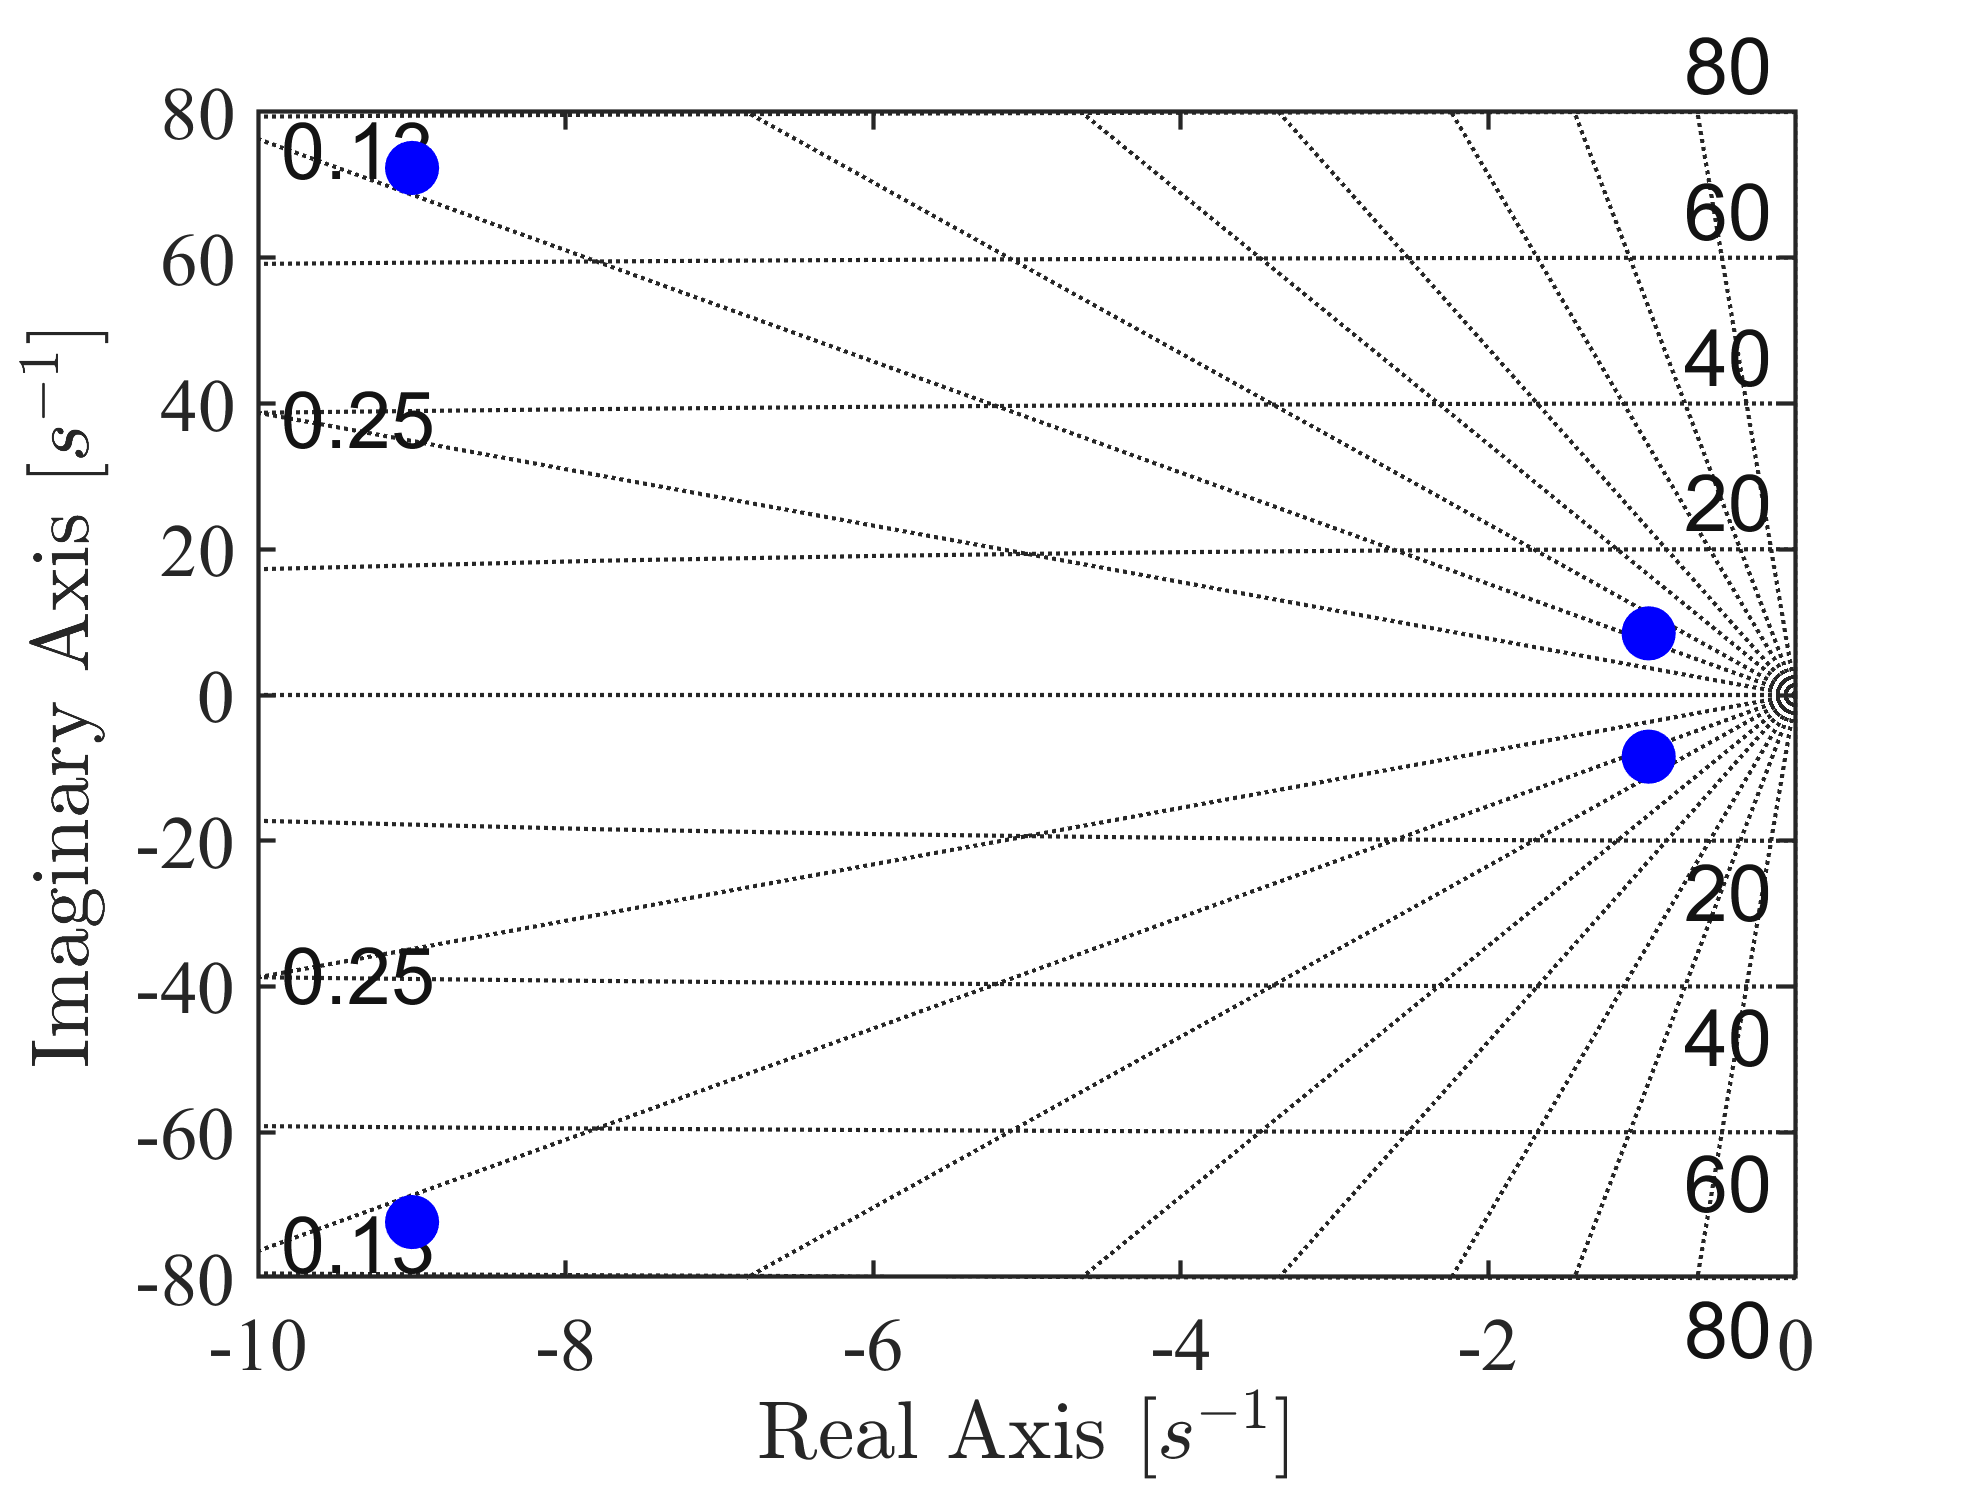
\includegraphics[width=7cm]{img/autovalores_malha_aberta.png}
            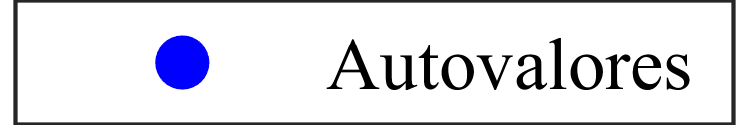
\includegraphics[width=3cm]{img/autovalores_malha_aberta_leg.png}
            \caption{Autovalores do sistema linearizado em malha aberta}
            \label{fig:autovalores_malha_aberta}
        \end{centering}
    \end{figure}
    \FloatBarrier
    
    Através do gráfico da figura \ref{fig:autovalores_malha_aberta}, pode-se observar que o sistema possui um par de autovalores dominantes, com frequência de oscilação da resposta de $8.4588 rad.s^{-1}$ e taxa de amortecimento de $0.1124$. Além disso, o sistema possui um outro par de autovalores não dominantes com frequência de oscilação da resposta de $72.3231 rad.s^{-1}$ e taxa de decaimento de $0.1235$
    
    \subsection{Análise da Controlabilidade e da observabilidade do sistema linearizado}
    
    Primeiramente definiremos a matriz $\mathbf{C}$ para termos como saída apenas os estados do sistema referentes a posição das massas suspensa e não suspensa, como demonstrado em \ref{eq:matriz_c} exibida a seguir:
     \FloatBarrier
    \begin{equation} \label{eq:matriz_c}
        \begin{split}
             \mathbf{C}=
        \end{split}
        \begin{bmatrix}
            1&0&0&0&\\
            0&0&1&0&\\
        \end{bmatrix}
    \end{equation}
    
    As matrizes de controlabilidade e observabilidade são definidas em \ref{eq:matriz_controlabilidade} e \ref{eq:matriz_observabilidade} exibidas a seguir:
    \begin{equation} \label{eq:matriz_controlabilidade}
        \begin{split}
             \mathbf{M_C}=
        \end{split}
        \begin{bmatrix}
            B& AB& A^2B& \cdots& A^{n-1}B&
        \end{bmatrix}
    \end{equation}

    \begin{equation} \label{eq:matriz_observabilidade}
        \begin{split}
             \mathbf{M_O}=
        \end{split}
        \begin{bmatrix}
            C&\\
            CA&\\
            CA^2&\\
            \vdots&\\
            CA^{n-1}&
        \end{bmatrix}
    \end{equation}

    O sistema definido pelas m,atrizes $A$, $B$ e $C$ é controlável se a matriz de controlabilidade $M_C$ tiver posto igual a $n=4$. O sistema será igualmente observável se a matriz de observabilidade $M_O$ tiver posto igual a $n=4$. Para o sistema definido pelo conjunto de parâmetros exibidos em \ref{eq:parametros} obtemos as matrizes $M_C$ e $M_O$ exibidas a seguir:
    \FloatBarrier
    \begin{equation} \label{eq:MC}
          \begin{split}
             \mathbf{M_C}=
        \end{split}
    \begin{smallmatrix}
                   0& -\frac{1}{290}&     \frac{231}{3364}&  \frac{679}{724}&\\  
      -\frac{1}{290}&  \frac{231}{3364}&  \frac{679}{724}&   -\frac{33366}{95}&\\
                   0&  \frac{1}{40}&     -\frac{231}{464}&  -\frac{11425}{91}&\\  
        \frac{1}{40}& -\frac{231}{464}&  -\frac{11425}{91}&  \frac{44200}{9}&\\
    \end{smallmatrix}
    \end{equation}
 
    \begin{equation} \label{eq:MO}
        \begin{split}
             \mathbf{M_O}=
        \end{split}
        \begin{smallmatrix}
           1&              0&              0&              0&\\
           0&              0&              1&              0&\\       
           0&              1&              0&              0&\\       
           0&              0&              0&              1&\\    
       -\frac{2350}{29}&   -\frac{70}{29}&      \frac{2350}{29}&   \frac{ 70}{29}&\\    
        \frac{1175}{2}&     \frac{35}{2}&      -\frac{10675}{2}&  -\frac{35}{2}&\\    
        \frac{43570}{27}&  -\frac{27725}{841}& -\frac{117713}{9}&  \frac{27725}{841}&\\
       -\frac{198889}{17}&  \frac{27725}{116}&  \frac{284473}{3}& -\frac{578725}{116}&\\
        \end{smallmatrix}
    \end{equation}

Dado que a ordem do sistema linearizado é $\mathbf{n}=4$, e como o $Rank(M_C)=4$ e $Rank(M_O)=4$, pode-se afirmar que o sistema linearizado é controlável e observável.

\subsection{Projeto de um controlador por realimentação de estados} \label{sc:projeto_controlador_full}

Escolheu-se definir os requisitos temporais para projeto do controlador por realimentação de estados separadamente para cada par de polos do sistema. Para o par de polos de resposta rápida, correspondentes à dinâmica da massa suspensa no eixo das rodas, deseja-se um valor de Máximo Overshoot $M_O \leq 10$ \% e Tempo de acomodação para a faixa de tolerância de 2 \% $T_S \leq 0.1$ s. Os resultados numéricos são apresentados com arredondamento na quarta casa decimal.

Dada a equação \ref{eq:MO} para o cálculo da Taxa de amortecimento para um valor de máximo overshoot dado, obtém-se o seguinte valor objetivo para $\xi$:

\begin{equation*}
    \xi=-\frac{ln\left(0.1\right)}{\sqrt{\pi^2+ln^2(0.1)}}=0.5912
\end{equation*}

Dada a equação \ref{eq:Ts2} para o cálculo da $\omega_n$ objetivo para um tempo de assentamento dado, obtém-se o seguinte valor objetivo para $\omega_n$:

\begin{equation*}
    \omega_n=-\frac{ln\left( 0.02*\sqrt{1-0.5912} \right)}{0.1*0.5912}=73.7409
\end{equation*}

A alocação dos polos $\lambda = \sigma \pm \omega_n.i$ é determinada a partir da aplicação dos valores encontrados nas equações \ref{eq:xi} e \ref{eq:wd} e \ref{eq:eign}

\begin{align} \label{eq:polos_de_xi}
     \lambda = \omega_n * (-\xi \pm \sqrt{1-\xi^2}.i)
\end{align}

Para os polos de resposta rápida obtemos:

\begin{align*} \label{eq:polos_nao_dominantes}
     \lambda_1 = -43.5923 + 47.1507*i\\
     \lambda_2 = -43.5923 - 47.1507*i\\
\end{align*}

Para os polos de resposta lenta, correspondentes a massa não suspensa do quarto de veiculo, deseja-se um valor de Máximo Overshoot $M_O \leq 10$ \% e Tempo de acomodação para a faixa de tolerância de 2 \% $T_S \leq 0.5$ s. Os resultados numéricos são apresentados com arredondamento na quarta casa decimal.

Calcula-se os coeficientes $\xi$ e $\omega_n$ da mesma forma que para os polos não dominantes assim obtendo os autovalores correspondentes:

\begin{equation*}
    \xi=-\frac{ln\left(0.1\right)}{\sqrt{\pi^2+ln^2(0.1)}}=0.5912
\end{equation*}

\begin{equation*}
    \omega_n=-\frac{ln\left( 0.02*\sqrt{1-0.5912} \right)}{0.5*0.5912}=14.7482
\end{equation*}

\begin{align*} \label{eq:polos_dominantes}
     \lambda_3 = -8.7185 + 9.4301*i\\
     \lambda_4 = -8.7185 - 9.4301*i\\
\end{align*}

Desta maneira obtemos a seguinte disposição de polos para o sistema em malha fechada:

\begin{equation} \label{eq:autovalores_malha_fechada}
        \begin{split}
             \lambda=\mathbf{eig(A-B_u*K)}=
        \end{split}
        \begin{bmatrix}
            -43.5923& + 47.1507i&\\
            -43.5923& - 47.1507i&\\
            -8.7185& + 9.4301i&\\
            -8.7185& - 9.4301i&\\
        \end{bmatrix}
    \end{equation}

Uma comparação entre os polos de malha aberta e malha fechada é exibida na figura \ref{fig:autovalores_malha_fechada} exibida a seguir.

    \FloatBarrier
    \begin{figure}[htbp]
        \begin{centering}
            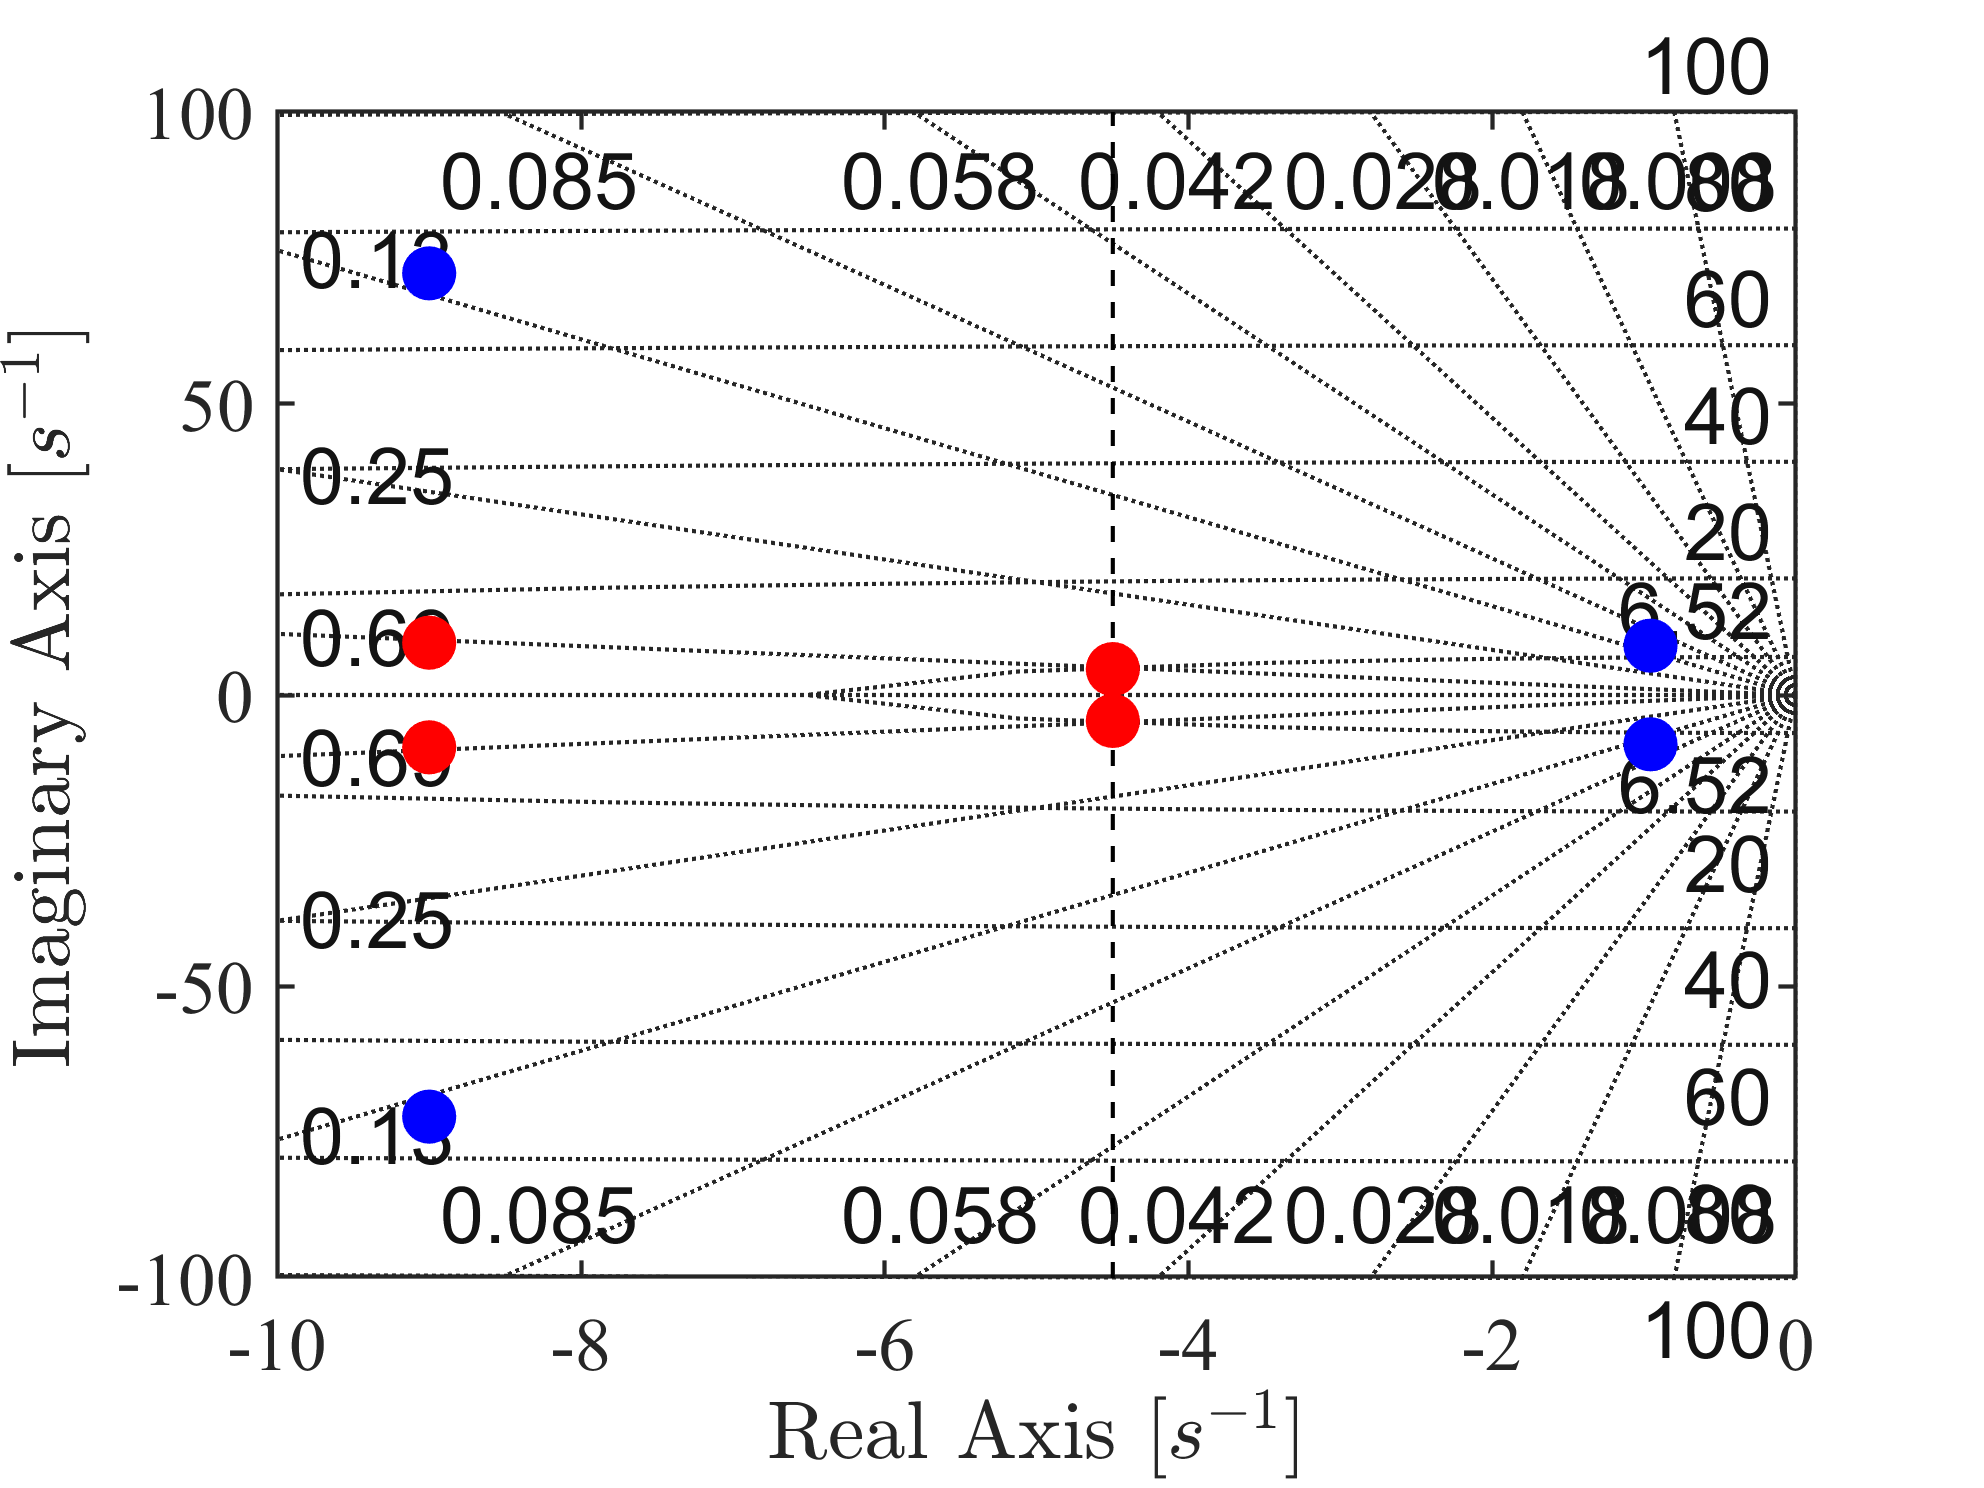
\includegraphics[width=7cm]{img/autovalores_malha_fechada.png}
            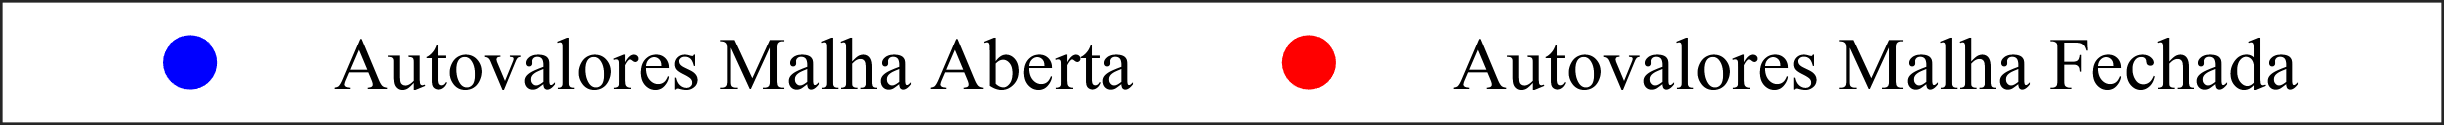
\includegraphics[width=6cm]{img/autovalores_malha_fechada_leg.png}
            \caption{Comparação entre os Autovalores do sistema linearizado em malha aberta e malha fechada}
            \label{fig:autovalores_malha_fechada}
        \end{centering}
    \end{figure}
    \FloatBarrier
    
    O ganho de realimentação para alocação de autovalores em malha fechada é computado através da equação de Lyapunov conforme descrito na seção \ref{sc:lyapunov} conforme exibido a seguir:
    
    \begin{equation*} 
    \begin{split}
        \mathbf{F} =
        \begin{bmatrix}
            -43.5923 &  47.1507 &       0       & 0 & \\ 
            -47.1507 & -43.5923 &       0 &       0 & \\
                   0 &        0 & -8.7185 &  9.4301 & \\
                   0 &        0 & -9.4301 & -8.7185 & \\
        \end{bmatrix}
    \end{split}
    \end{equation*} 
 
    \begin{equation*} 
    \begin{split}
        \mathbf{B} = B_u = 
        \begin{bmatrix}
            0 & \\
            -\frac{1}{m_s}&\\ \\
            0 & \\
            \frac{1}{m_u} \\
        \end{bmatrix};\ \
    \end{split}
    \begin{split}
    \mathbf{\bar{K}} =
        \begin{bmatrix}
        1&0&1&0&
        \end{bmatrix}
    \end{split}
    \end{equation*} 
    
    Resolvendo a equação de Lyapunov \ref{eq:lyapunov} para $T$ e substituindo a matriz T encontrada na equação \ref{eq:ganho} obtém-se os seguintes valores de ganhos de realimentação, valores arredondados na quarta casa decimal:
    
    \begin{center}
    \begin{tabular}{|c|c|}
        \hline
        Estado & Ganho\\
        \hline
        \hline
        $x_1$    & -18023.2837\\
        $x_2$    & -4567.6793\\
        $x_3$    & 13118.63414\\   
        $x_4$    & 2758.2869 \\
        \hline
    \end{tabular}
    \end{center}
    
    \subsection{Simulação da resposta temporal do modelo linearizado em malha fechada com controlador por realimentação de estados} \label{sc:analise_resposta}
    
    Abaixo seguem gráficos que ilustram a simulação temporal da resposta do sistema linearizado para excitação com entrada em "lombada" degrau de 0.1m:
    \FloatBarrier
    \begin{figure}[htbp]
        \begin{centering}
            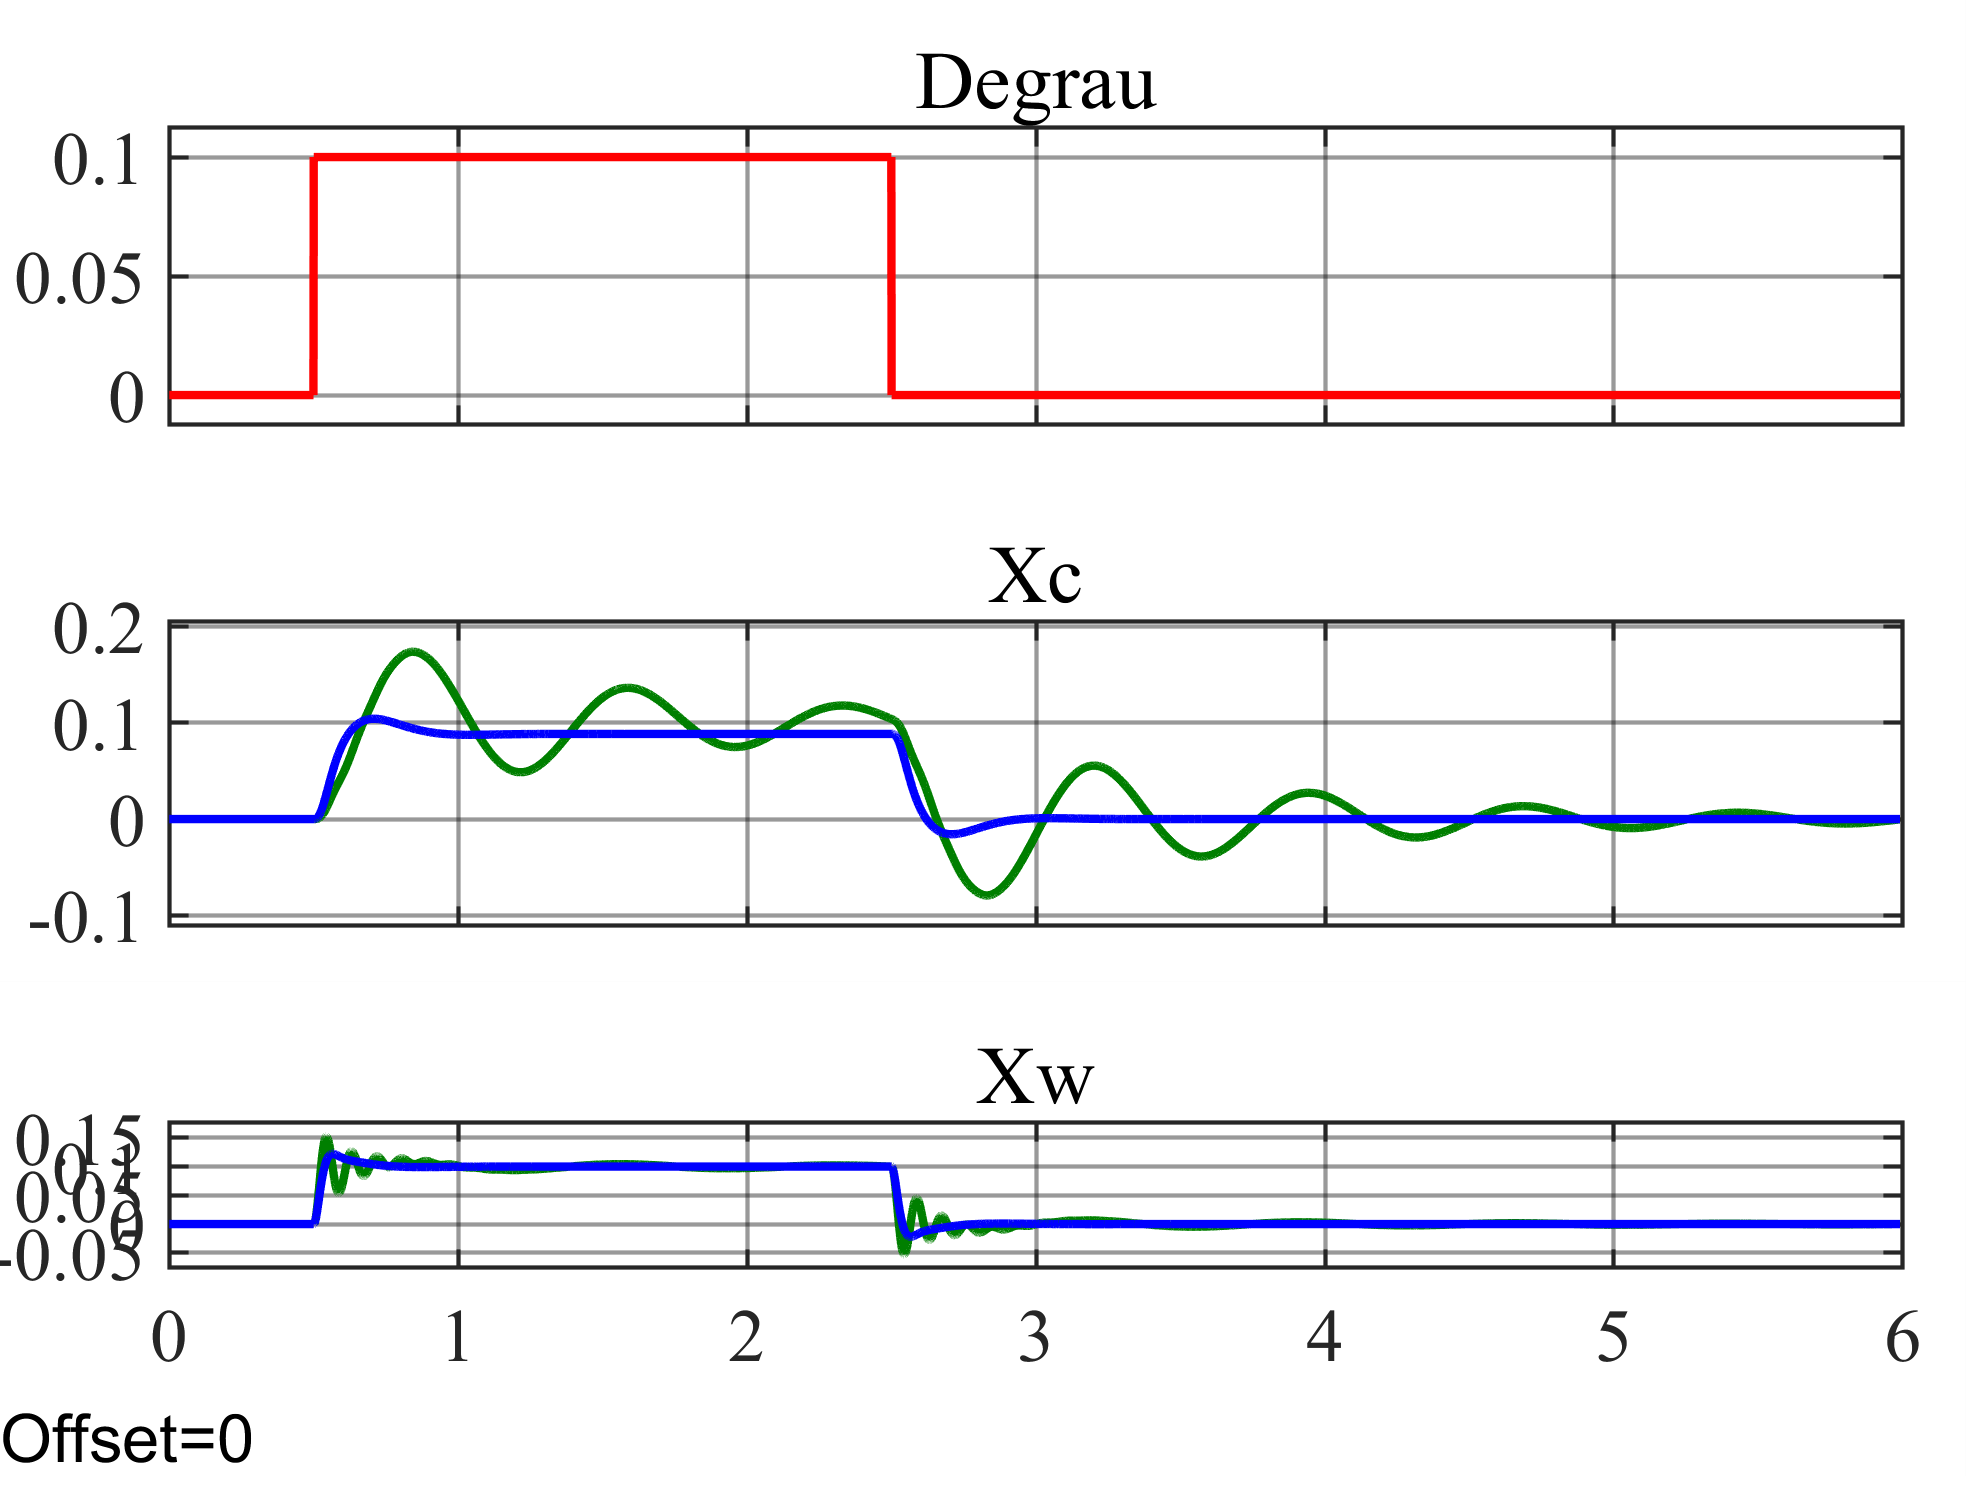
\includegraphics[width=8cm]{img/simulaca_temporal_linear_realimentacao.png}
            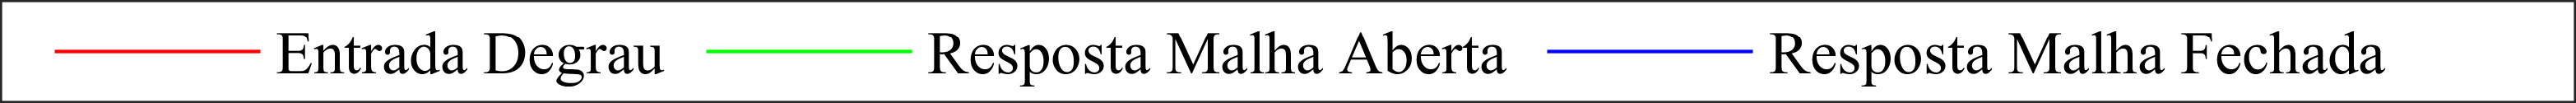
\includegraphics[width=8cm]{img/sim_linear_simulink_temp_leg.png}
            \caption{Simulação da resposta temporal em malha fechada com o controlador projetado na subseção \ref{sc:projeto_controlador_full} para o sistema linearizado.Estados $x_c$ e $x_w$ }
            \label{fig:simulaca_temporal_linear_realimentacao}
        \end{centering}
    \end{figure}
    \FloatBarrier
	
	\FloatBarrier
    \begin{figure}[htbp]
        \begin{centering}
            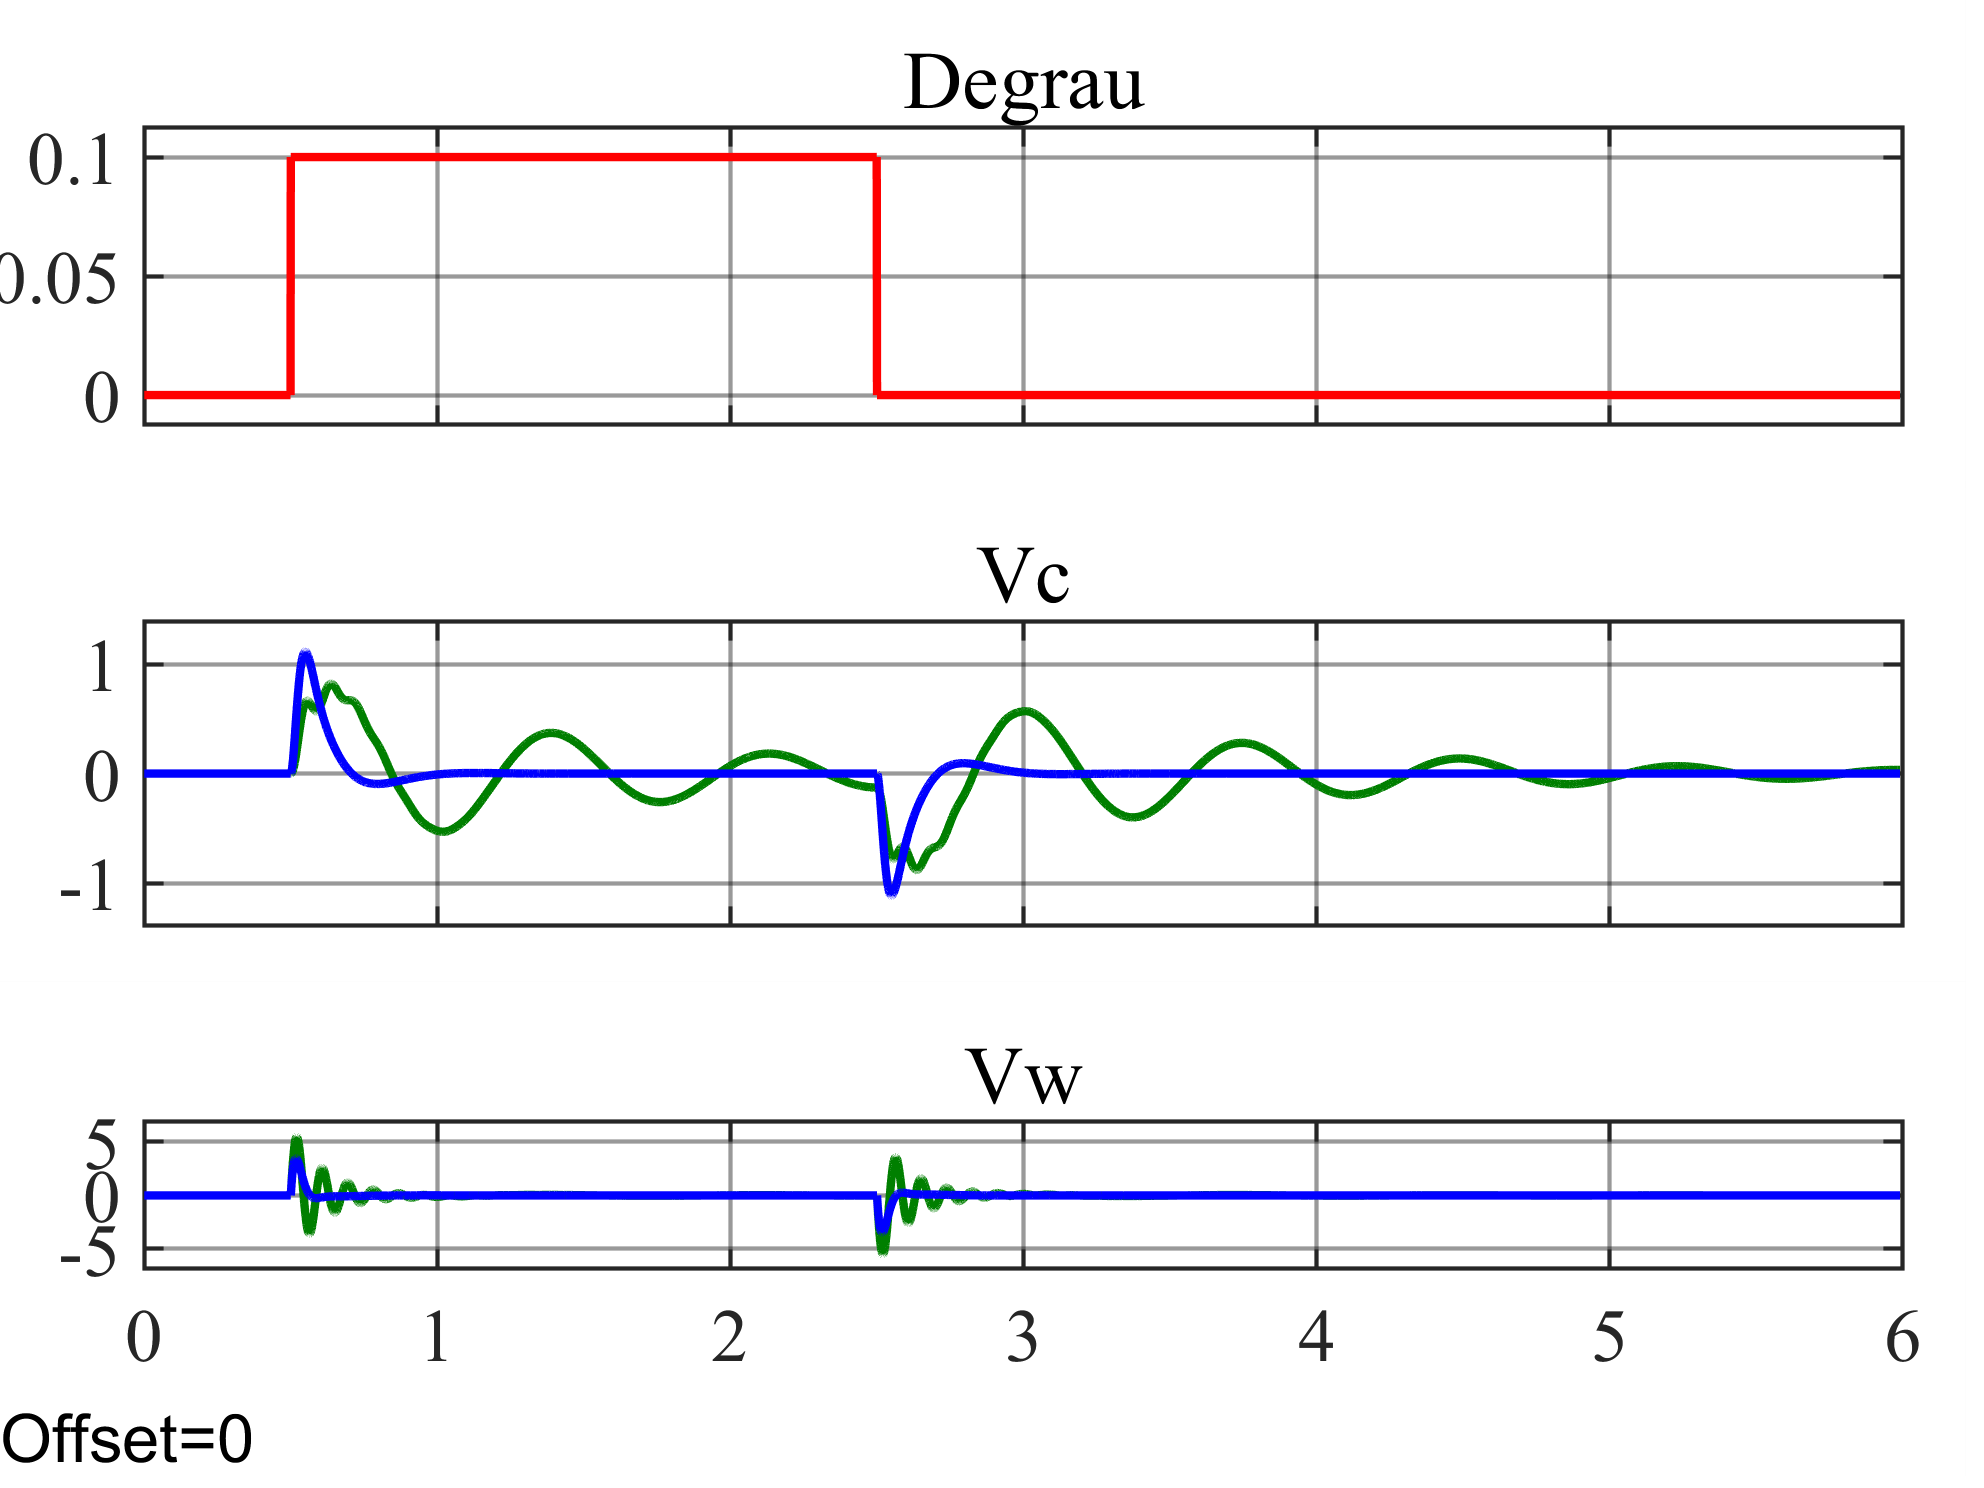
\includegraphics[width=8cm]{img/simulaca_temporal_linear_realimentacao_V.png}
            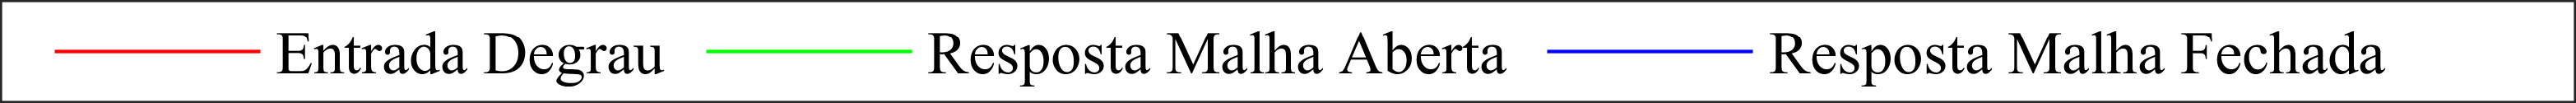
\includegraphics[width=8cm]{img/sim_linear_simulink_temp_leg.png}
            \caption{Simulação da resposta temporal em malha fechada com o controlador projetado na subseção \ref{sc:projeto_controlador_full} para o sistema linearizado.Estados $V_c = \dot{x}_c$ e $V_w = \dot{x}_w$ }
            \label{fig:simulaca_temporal_linear_realimentacao_V}
        \end{centering}
    \end{figure}
    \FloatBarrier
    
    A observação dos gráficos da resposta temporal exibida nas figuras \ref{fig:simulaca_temporal_linear_realimentacao} e \ref{fig:simulaca_temporal_linear_realimentacao_V} traz algumas considerações, enumerados a seguir:
    
    \begin{itemize}
        \item A realimentação de estados, na forma em que foi projetada, preservou a estabilidade do sistema.
        \item A realimentação de estados sozinha foi capaz de alterar os polos, ou autovalores, do sistema para as localizações desejadas.
        \item A nova localização dos polos, ou autovalores, foi capaz de alterar as frequências de resposta forçada do sistema. Isso contribuiu para que este atingisse a estabilização da resposta transitória mais rapidamente do que quando em malha aberta, atingindo as especificações do tempo de assentamento.
        \item A nova localização dos polos, ou autovalores, foi capaz de atenuar mais rapidamente as frequências de resposta forçada do sistema. Isso contribuiu para que este atingisse a estabilização da resposta transitória mais rapidamente do que quando em malha aberta além de ser capaz de reduzir o overshoot.
        \item A realimentação de estados sozinha não foi capaz de zerar o erro do estado $\dot{x}_c$ para referência zero quando o sistema foi excitado por um degrau. O que não aconteceu para o sistema em malha aberta. Considerando que o sistema de coordenadas é relativo ao sistema de coordenadas do solo e ao offset inicial de cada componente, espera-se que em regime permanente os estados $x_c$ e $x_w$ estejam na mesma posição que a excitação em $x_r$.
        \item A realimentação de estados tornou o sistema mais rápido por um curto espaço de tempo durante o tempo de subida. Apesar de estar sujeito a um menor overshoot, as massas do sistema sofreram maiores acelerações de pico durante o transitório.
    \end{itemize}
    
    De uma maneira geral a resposta do sistema controlado é bastante satisfatória.
    
    \subsection{Simulação da resposta temporal do sistema em malha fechada considerando o sistema não linear original utilizando o controlador projetado para o sistema linear}
    
    Abaixo seguem gráficos que ilustram a simulação temporal da resposta do sistema não linear comparada com a resposta do sistema linearizado para excitação com entrada em "lombada" degrau de 0.1m:
    
    \FloatBarrier
    \begin{figure}[htbp]
        \begin{centering}
            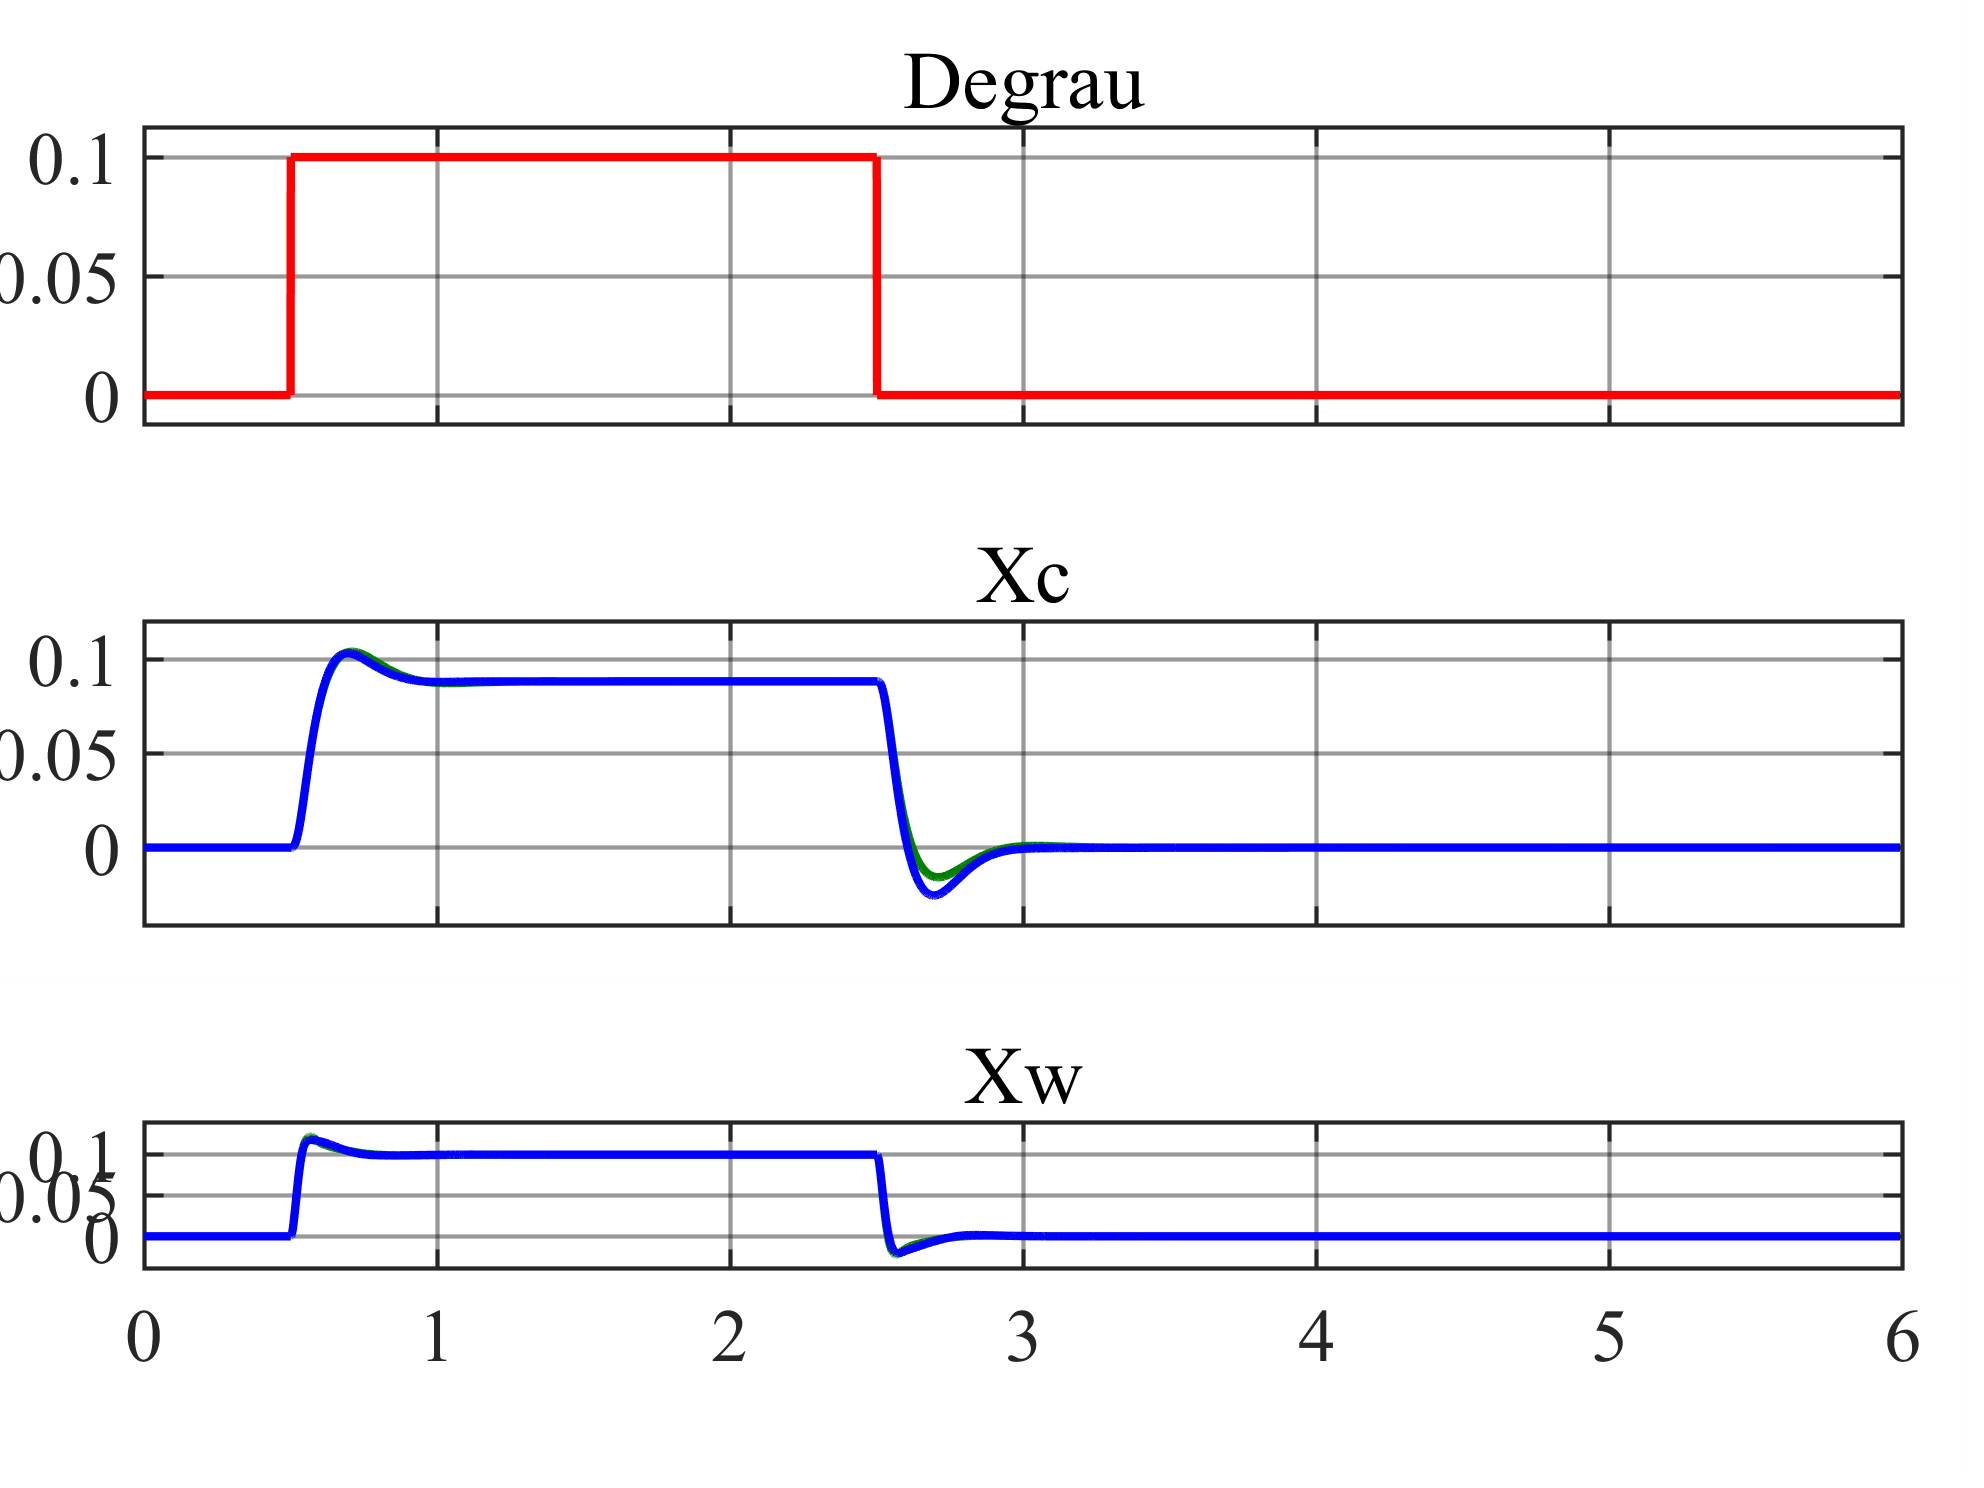
\includegraphics[width=7cm]{img/simulaca_temporal_nao_linear_realimentacao.png}
            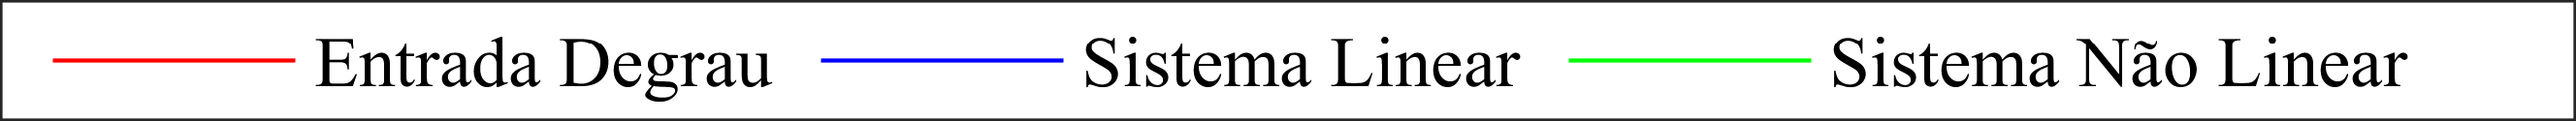
\includegraphics[width=6cm]{img/sim_nao_linear_simulink_temp_leg.png}
            \caption{Simulação da resposta temporal em malha fechada com o controlador projetado na subseção \ref{sc:projeto_controlador_full} para o sistema linearizado e não linearizado.Estados $x_c$ e $x_w$ }
            \label{fig:simulaca_temporal_nao_linear_realimentacao}
        \end{centering}
    \end{figure}
    \FloatBarrier
	
	\FloatBarrier
    \begin{figure}[htbp]
        \begin{centering}
            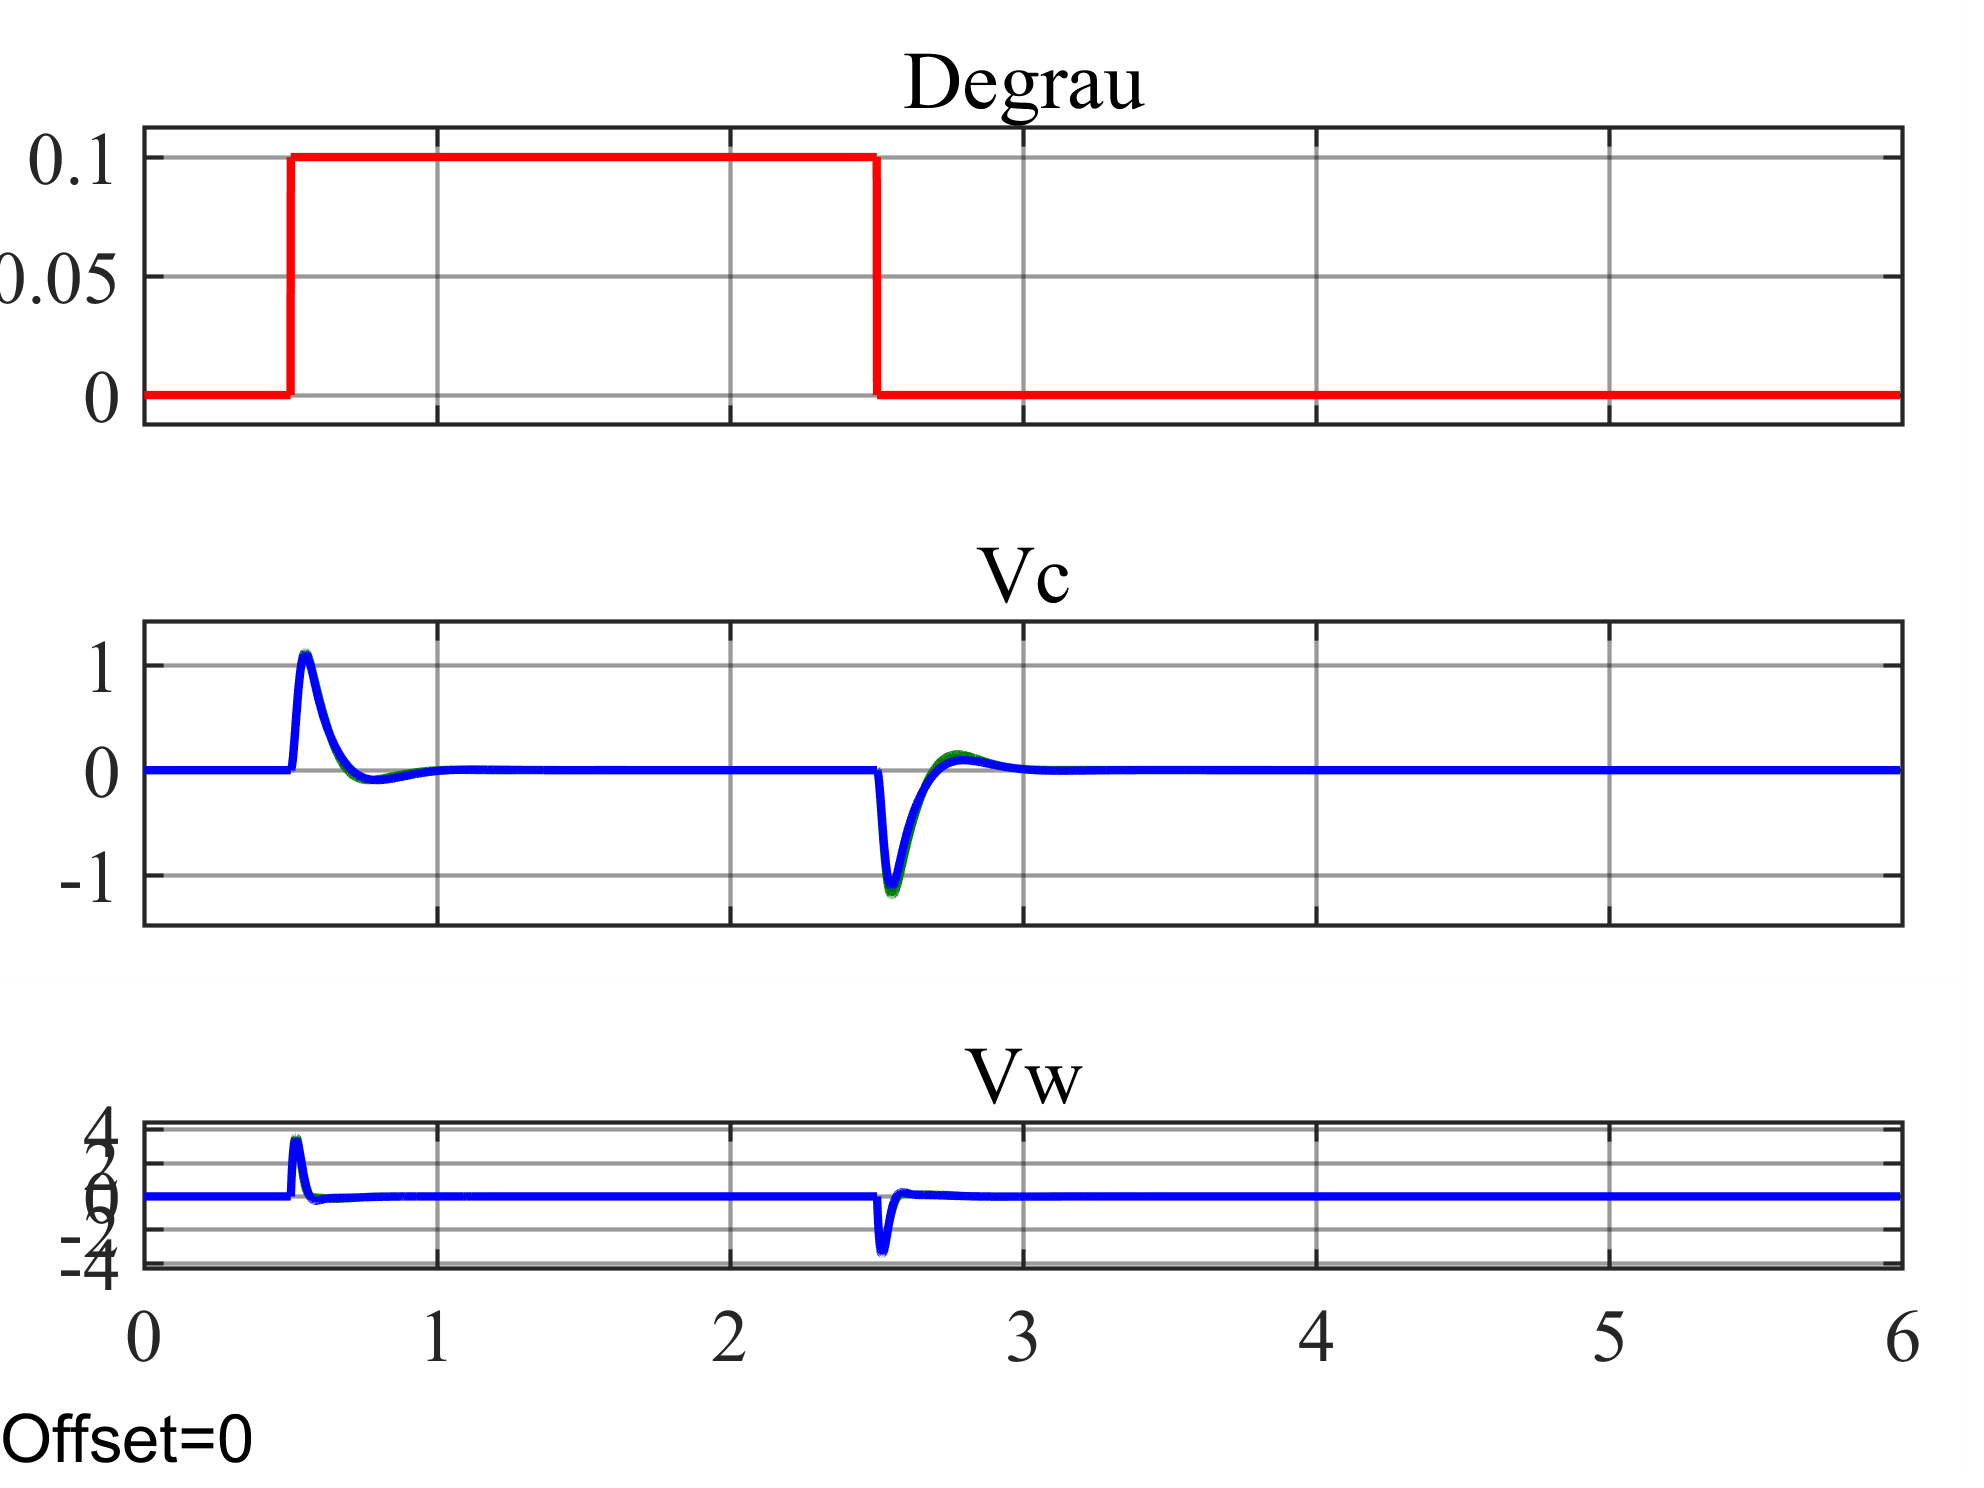
\includegraphics[width=7cm]{img/simulaca_temporal_nao_linear_realimentacao_V.png}
            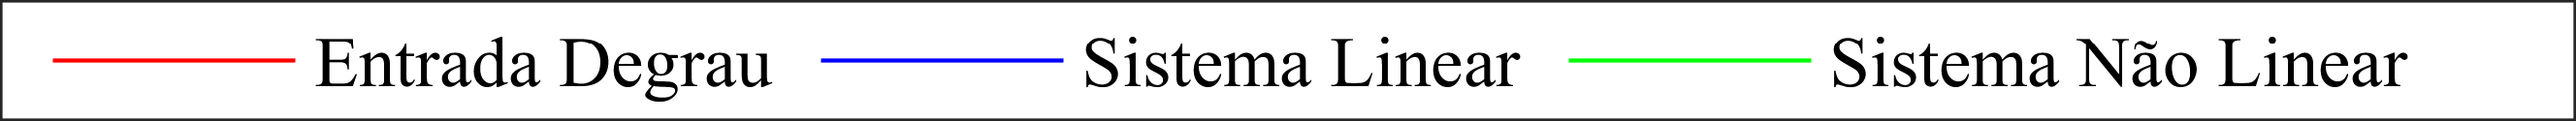
\includegraphics[width=6cm]{img/sim_nao_linear_simulink_temp_leg.png}
            \caption{Simulação da resposta temporal em malha fechada com o controlador projetado na subseção \ref{sc:projeto_controlador_full} para o sistema linearizado e não linearizado.Estados $V_c = \dot{x}_c$ e $V_w = \dot{x}_w$ }
            \label{fig:simulaca_temporal_nao_linear_realimentacao_V}
        \end{centering}
    \end{figure}
    \FloatBarrier
    
    A observação dos gráficos da resposta temporal exibida nas figuras \ref{fig:simulaca_temporal_nao_linear_realimentacao} e \ref{fig:simulaca_temporal_nao_linear_realimentacao_V} traz a conclusão que, para este caso especifico, a resposta temporal do sistema não linear em malha fechada com o controlador projetado para o sistema linearizado se mostrou muito semelhante a resposta temporal do sistema linear. Neste caso, contribuíram para isto a excitação com "lombada" em degrau pequena afastou pouco o sistema do ponto de equilíbrio, ao mesmo tempo que um controlador com um amortecimento relativamente alto, $\xi \simeq 0.6$, contribuiu para que a resposta transitória rica em frequências fosse rapidamente cancelada e apenas o comportamento em regime fosse exibido a maior parte do tempo.
    
    Para comparação, é exibido a seguir a mesma simulação temporal para uma entrada com "lombada" em degrau unitário. Esta entrada excita mais frequências de ambos os sistema e podem revelar mais informações sobre as diferenças entre ambos os sistemas pois leva o sistema linearizado para uma condição de operação mais afastada do ponto de equilíbrio: 
    
    \FloatBarrier
    \begin{figure}[htbp]
        \begin{centering}
            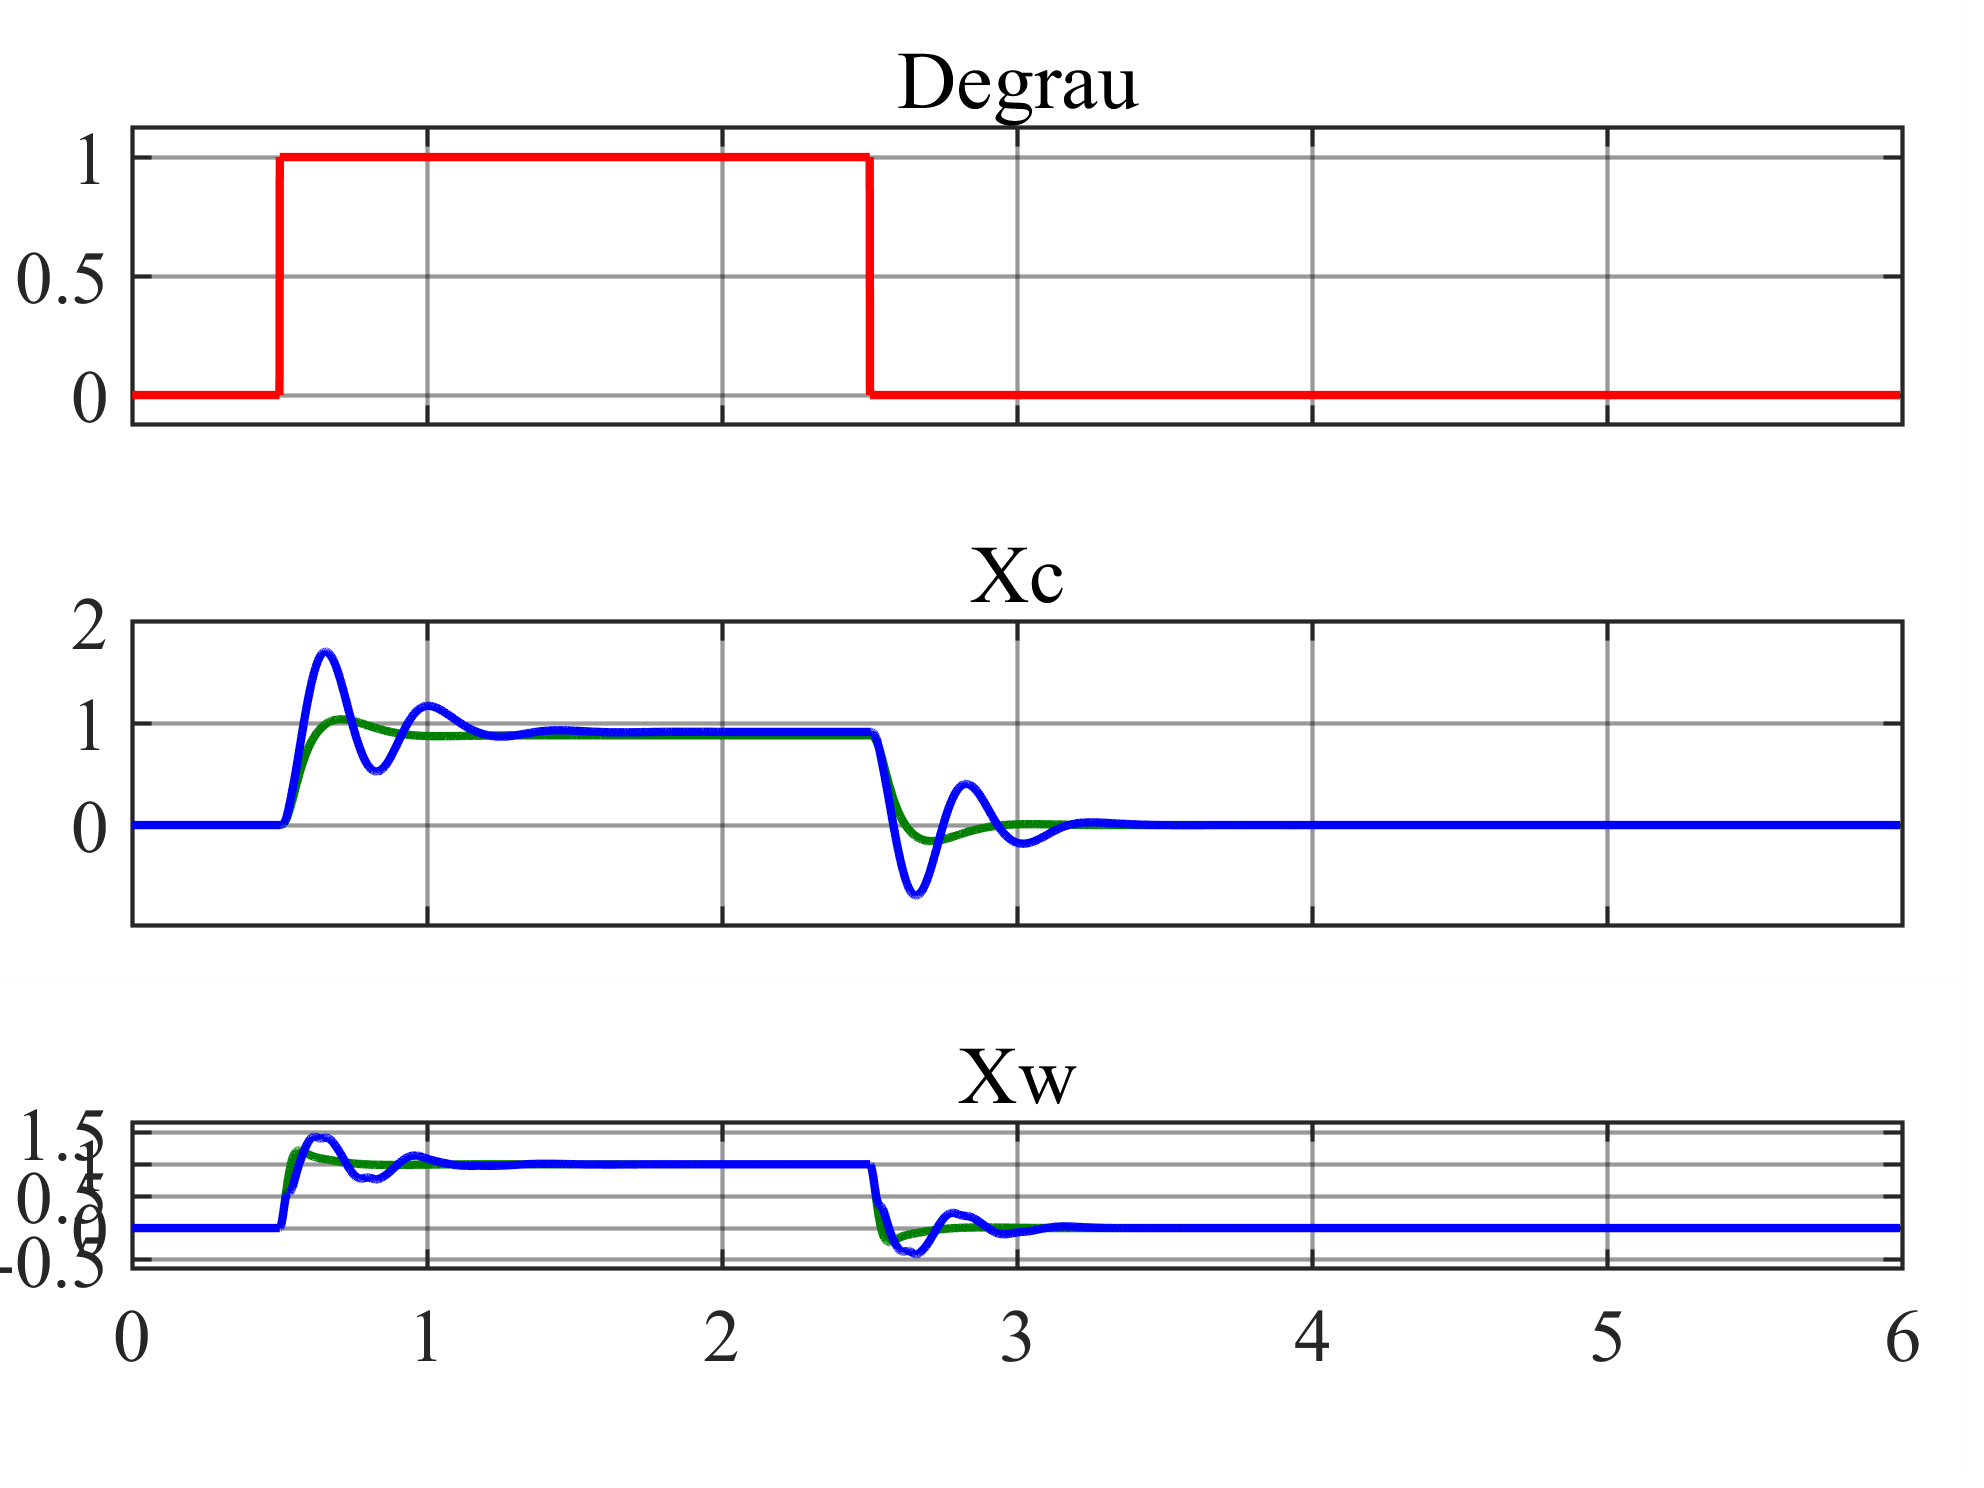
\includegraphics[width=7cm]{img/simulaca_temporal_nao_linear_realimentacao_unit.png}
            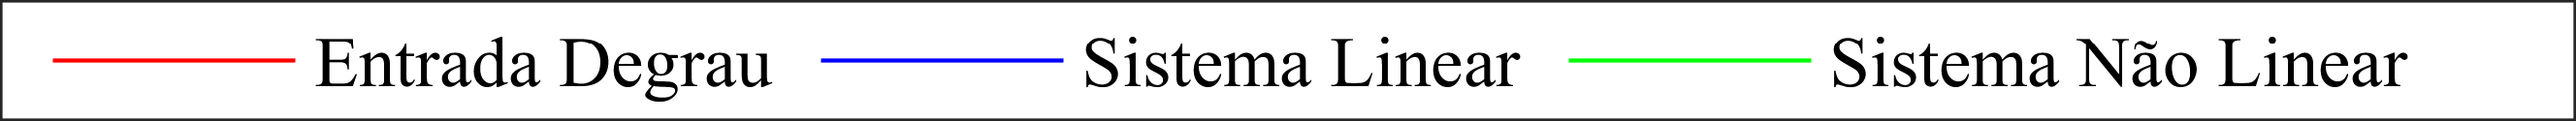
\includegraphics[width=6cm]{img/sim_nao_linear_simulink_temp_leg.png}
            \caption{Simulação da resposta temporal em malha fechada com o controlador projetado na subseção \ref{sc:projeto_controlador_full} para o sistema linearizado e não linearizado.Estados $x_c$ e $x_w$ }
            \label{fig:simulaca_temporal_nao_linear_realimentacao_unit}
        \end{centering}
    \end{figure}
    \FloatBarrier
	
	\FloatBarrier
    \begin{figure}[htbp]
        \begin{centering}
            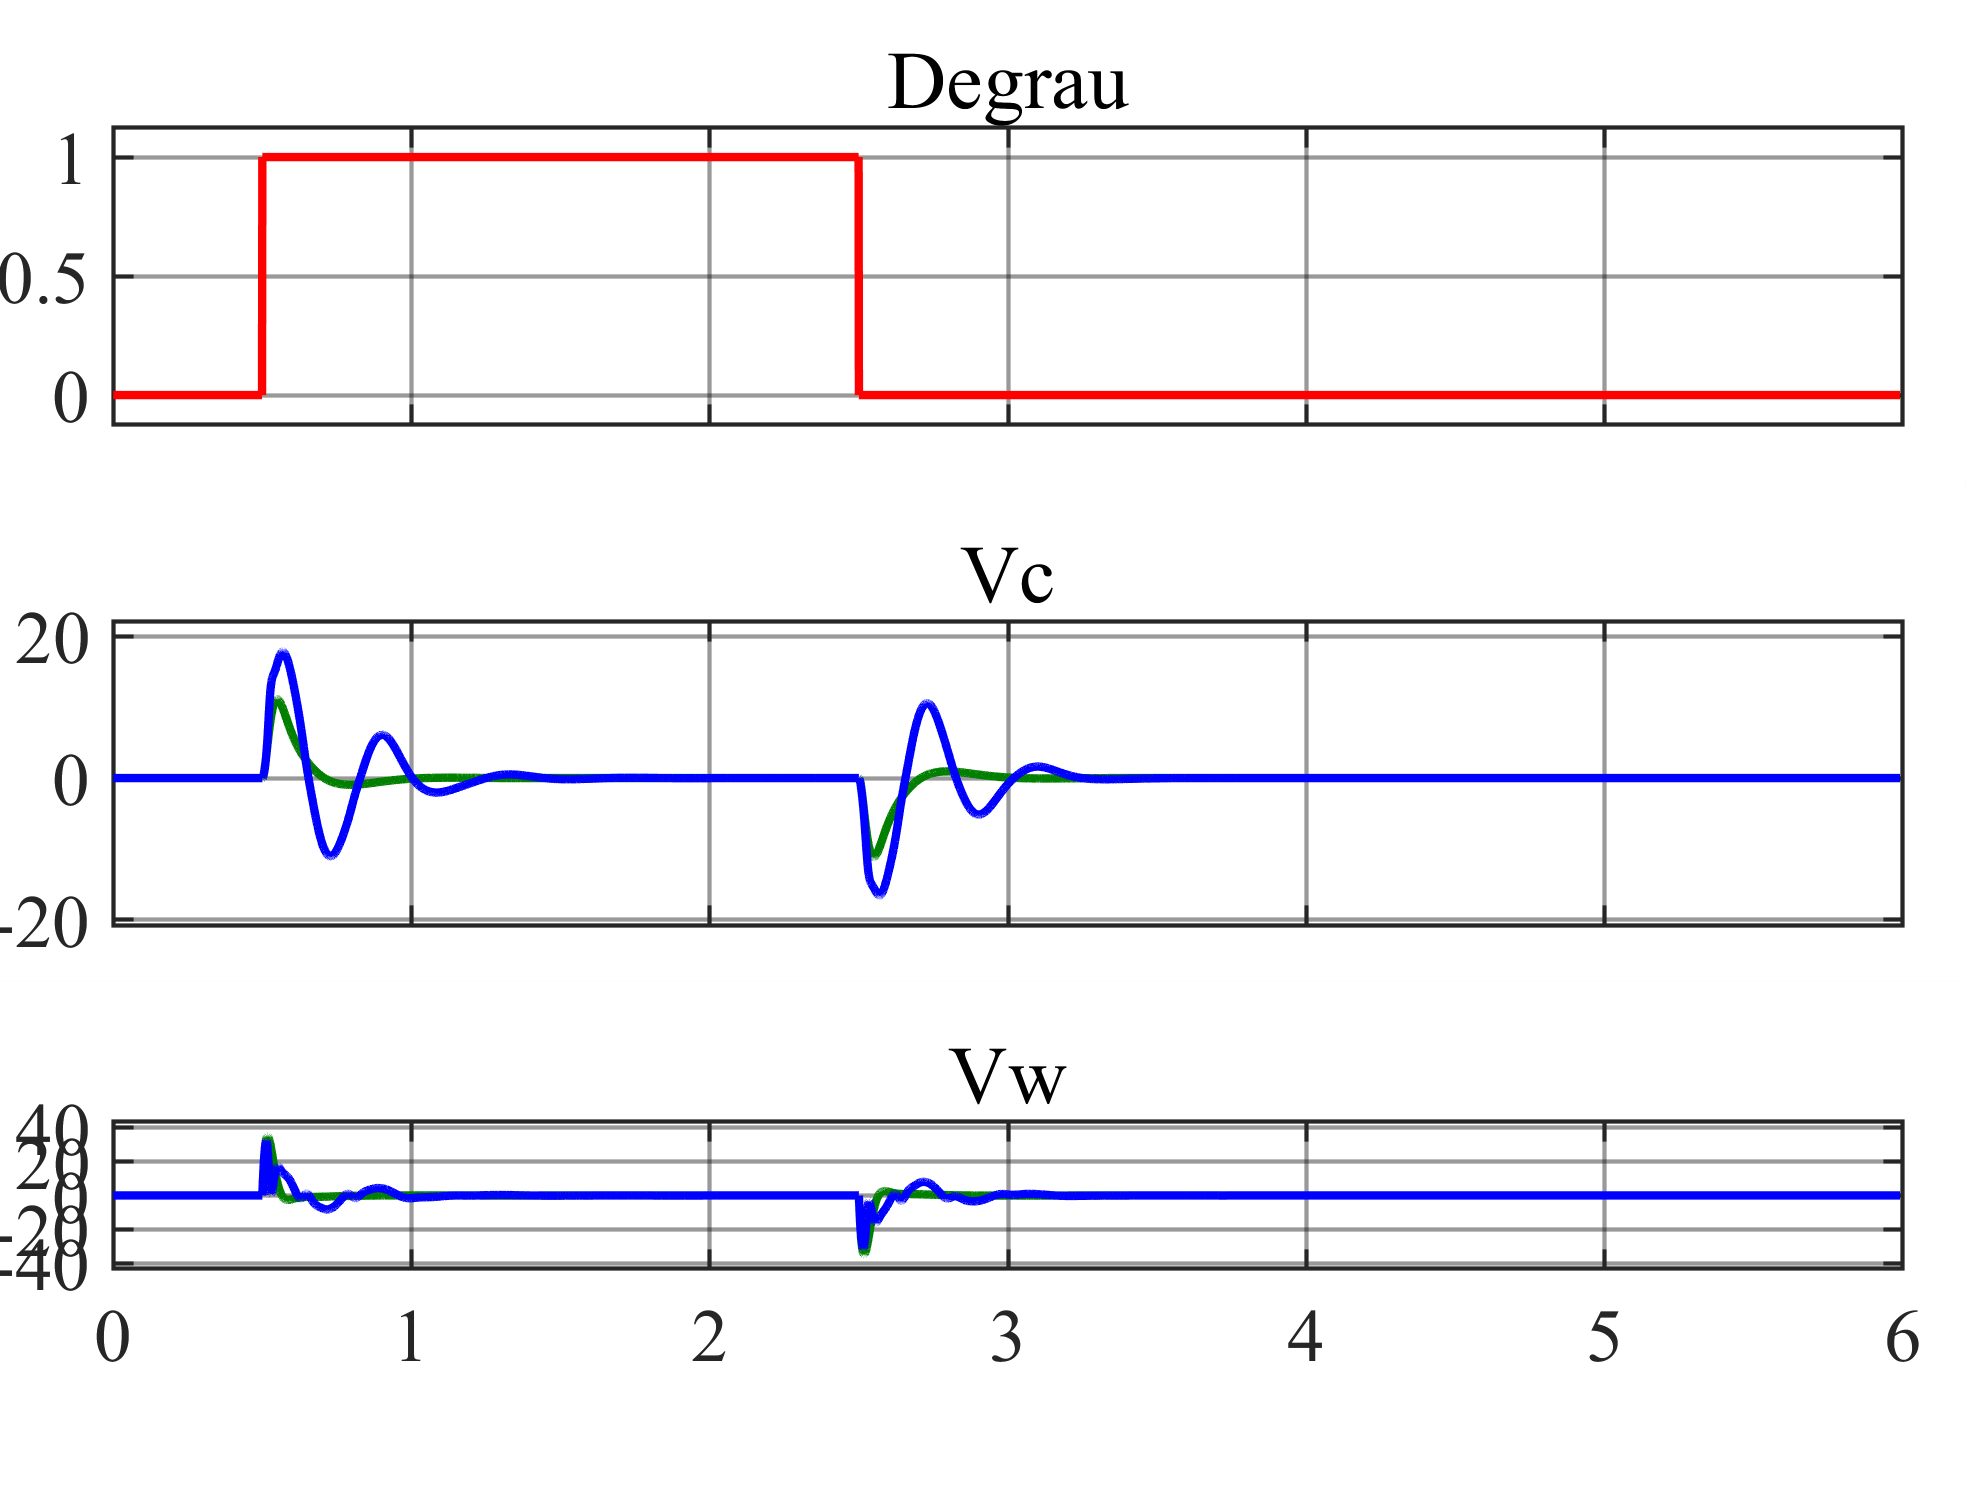
\includegraphics[width=7cm]{img/simulaca_temporal_nao_linear_realimentacao_unit_V.png}
            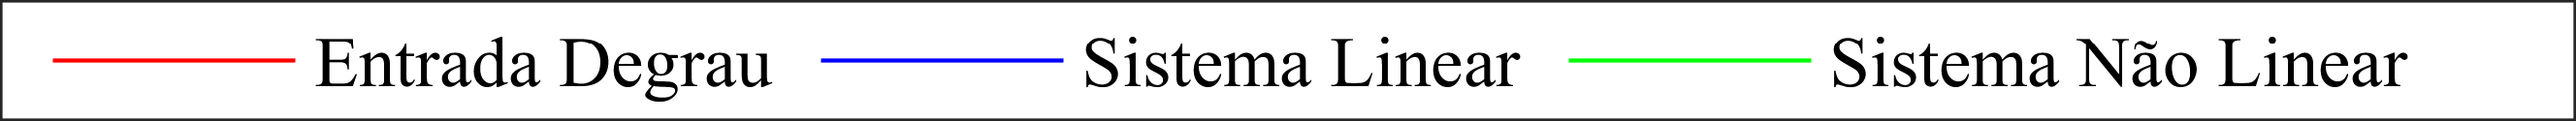
\includegraphics[width=6cm]{img/sim_nao_linear_simulink_temp_leg.png}
            \caption{Simulação da resposta temporal em malha fechada com o controlador projetado na subseção \ref{sc:projeto_controlador_full} para o sistema linearizado e não linearizado.Estados $V_c = \dot{x}_c$ e $V_w = \dot{x}_w$ }
            \label{fig:simulaca_temporal_nao_linear_realimentacao_unit_V}
        \end{centering}
    \end{figure}
    \FloatBarrier
    
    A observação dos gráficos da resposta temporal exibida nas figuras \ref{fig:simulaca_temporal_nao_linear_realimentacao_unit} e \ref{fig:simulaca_temporal_nao_linear_realimentacao_unit_V} demonstra que para uma entrada que desloque o sistema para uma região muito distante do ponto de equilíbrio utilizado para linearização pode causar uma grande diferença na resposta temporal do controle em malha fechada, inclusive podendo degradar significativamente o desempenho do controlador por realimentação de estados. 

 \subsection{Simulação da resposta temporal em malha fechada com o controlador projetado para o sistema linearizado e considerando perturbação}
 
Abaixo seguem gráficos que ilustram a simulação temporal da resposta do sistema linearizado para excitação com perturbações em degraus aleatórios entre $\pm$ 5cm.

\FloatBarrier
    \begin{figure}[htbp]
        \begin{centering}
            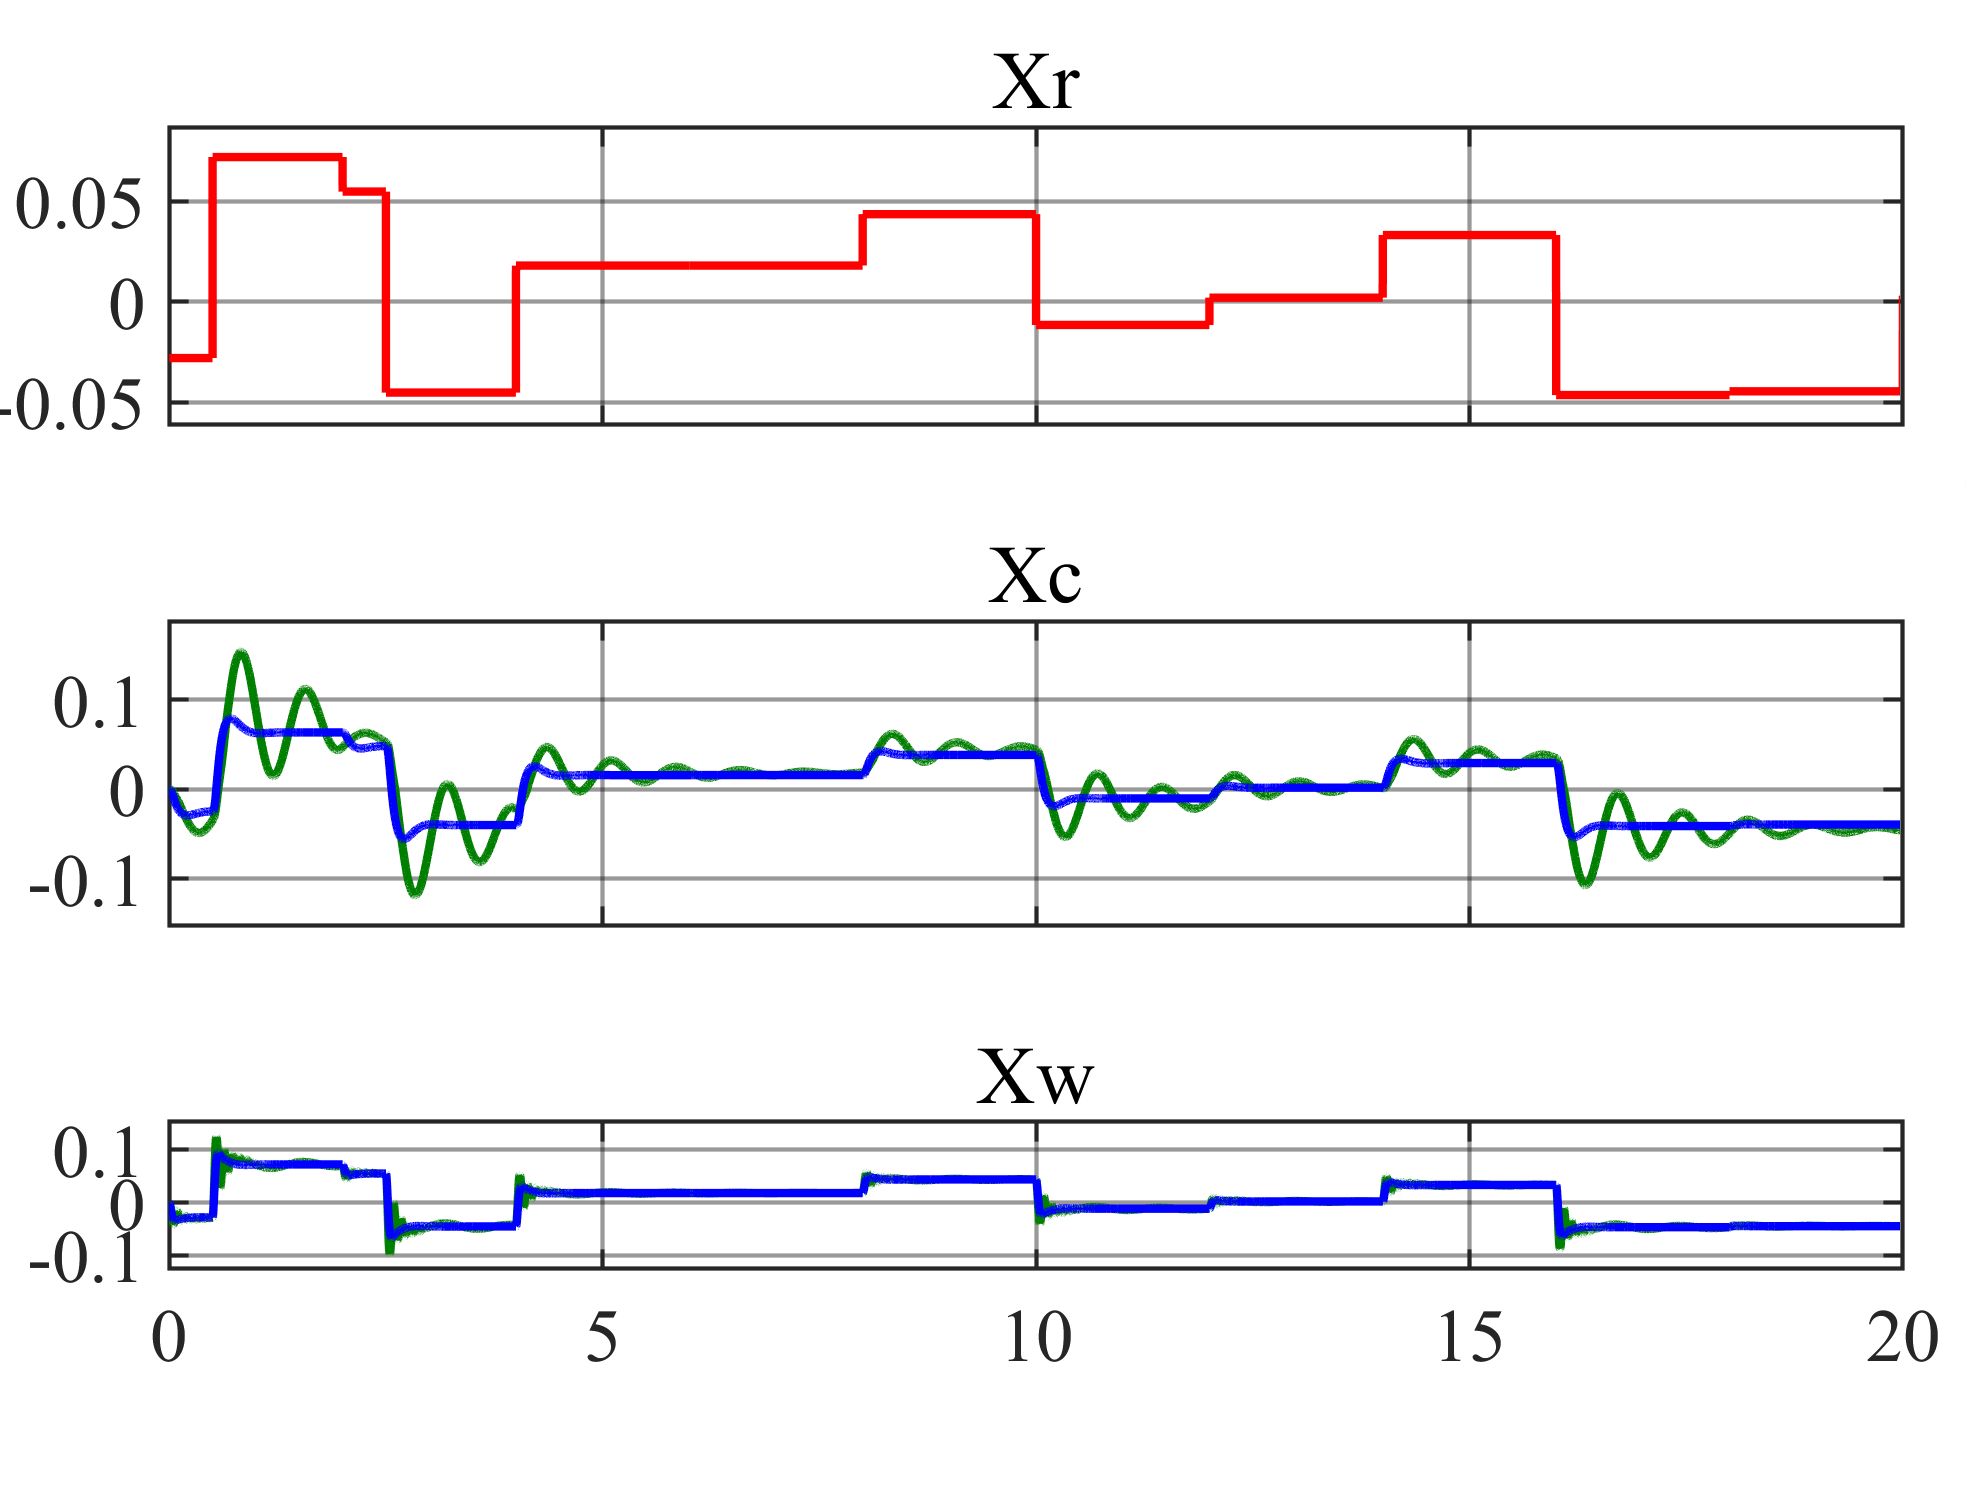
\includegraphics[width=8cm]{img/simulaca_temporal_linear_perturbacao.png}
            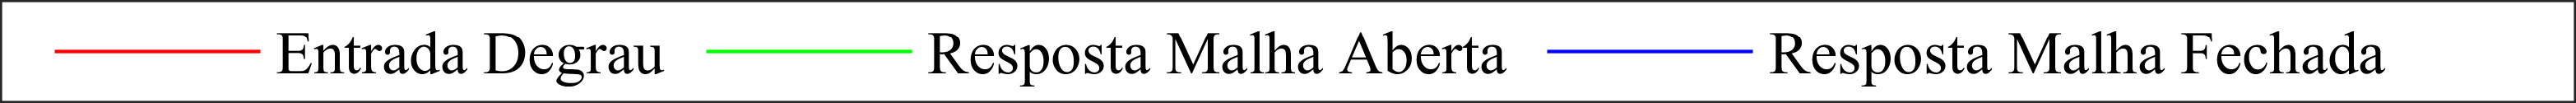
\includegraphics[width=7cm]{img/sim_linear_simulink_temp_leg.png}
            \caption{Simulação da resposta temporal com o controlador projetado na subseção \ref{sc:projeto_controlador_full} para o sistema linearizado em malha aberta e malha fechada.Estados $X_c = \dot{x}_c$ e $X_w = \dot{x}_w$ }
            \label{fig:simulaca_temporal_linear_perturbacao}
        \end{centering}
    \end{figure}
    \FloatBarrier
\FloatBarrier
    \begin{figure}[htbp]
        \begin{centering}
            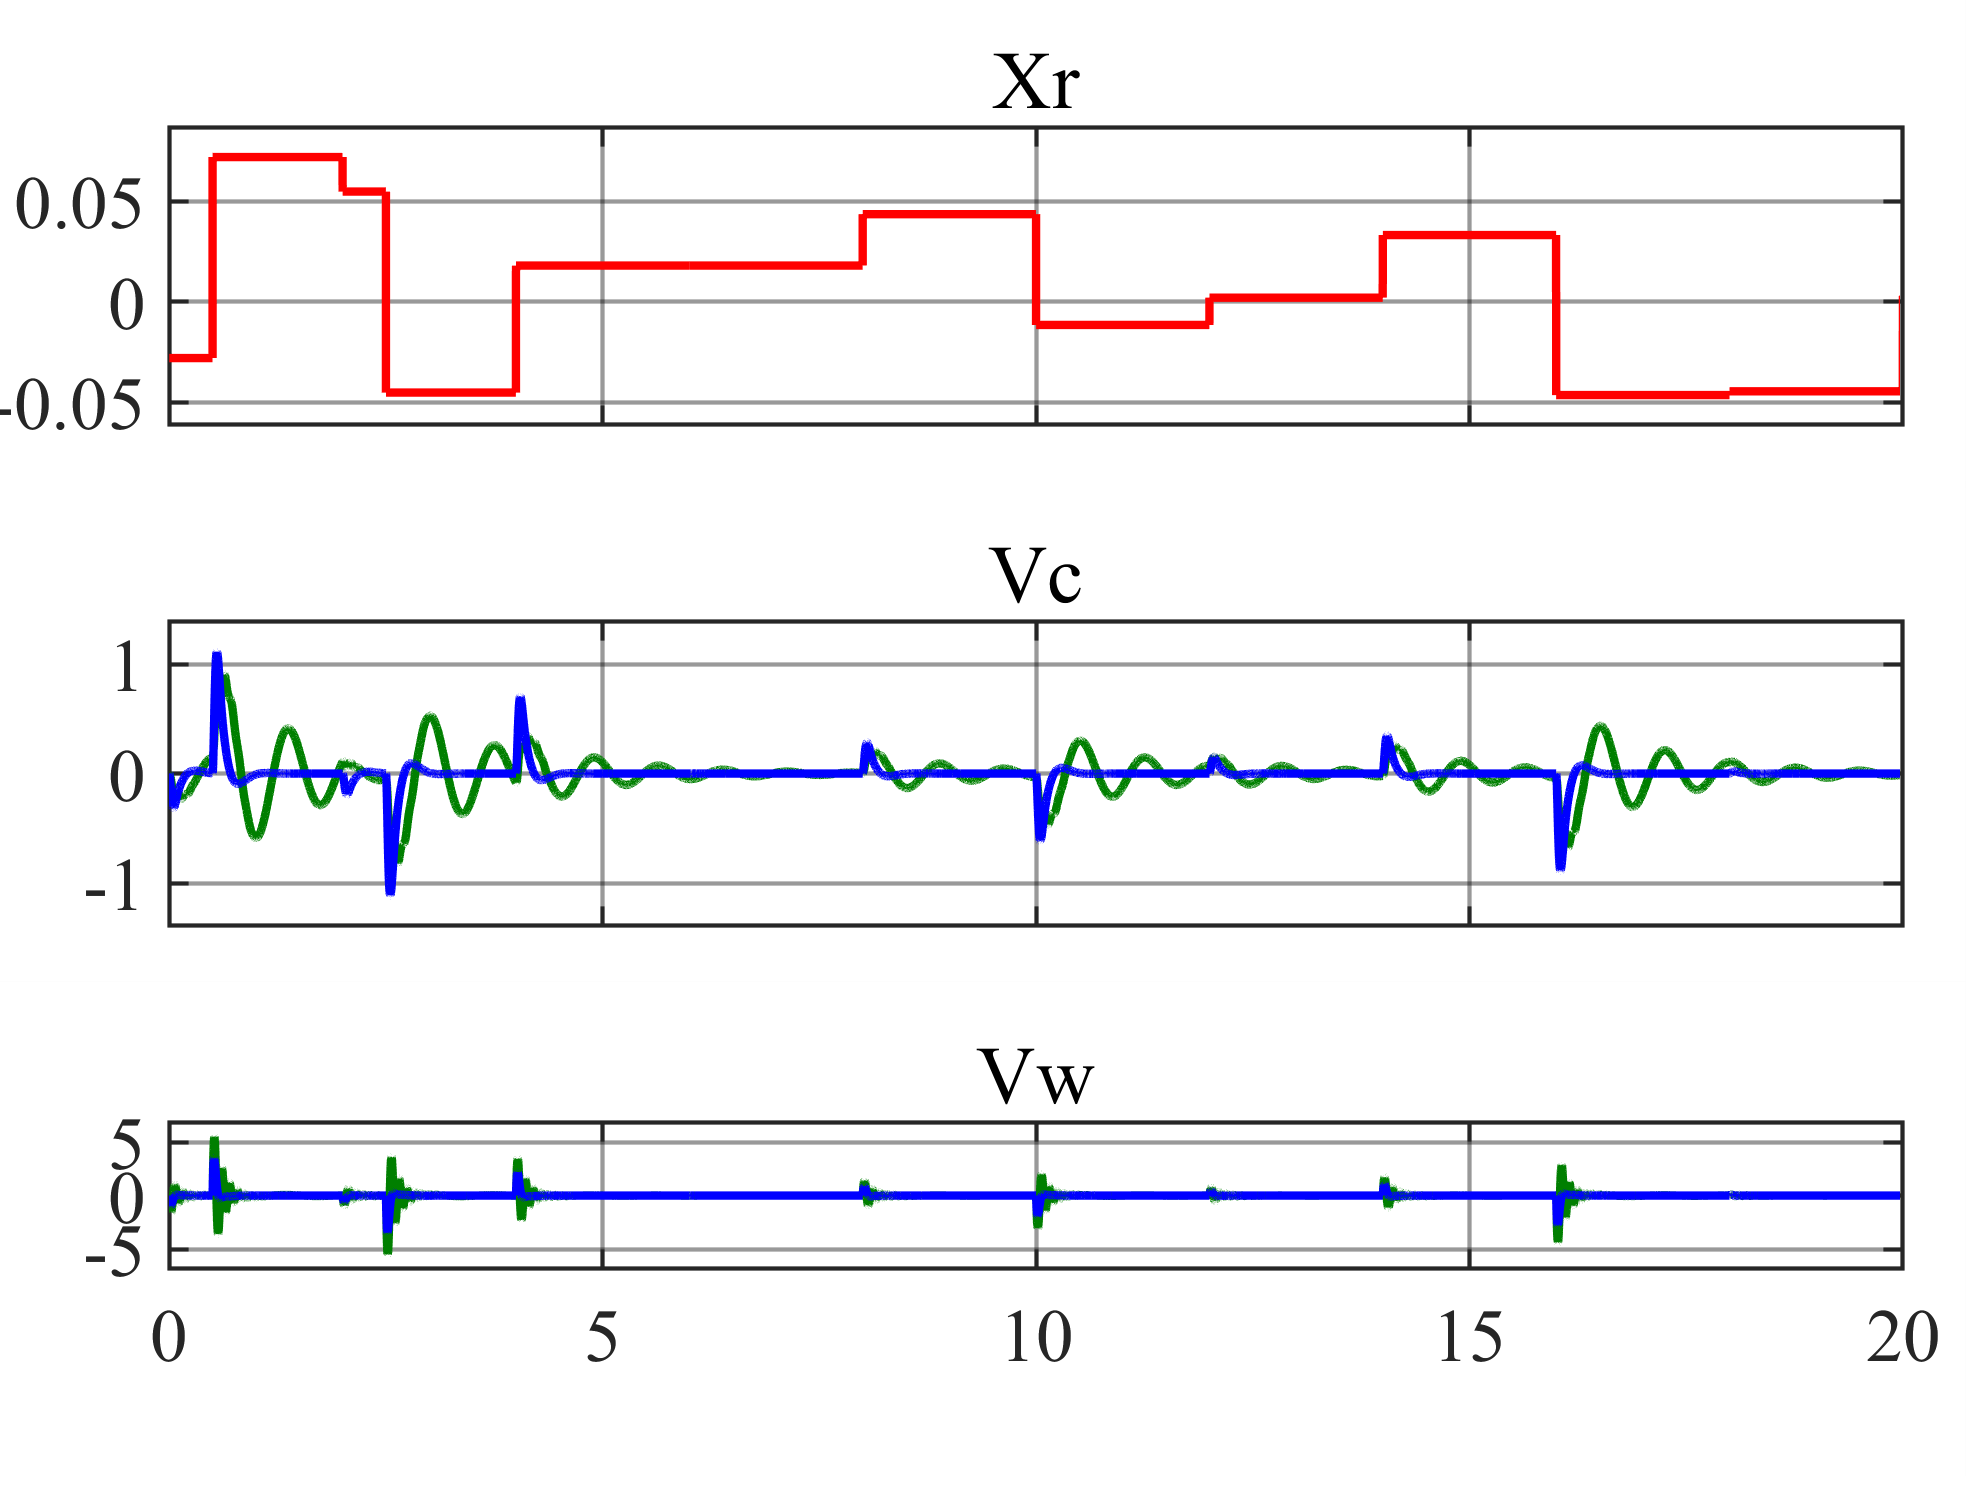
\includegraphics[width=8cm]{img/simulaca_temporal_linear_perturbacao_V.png}
            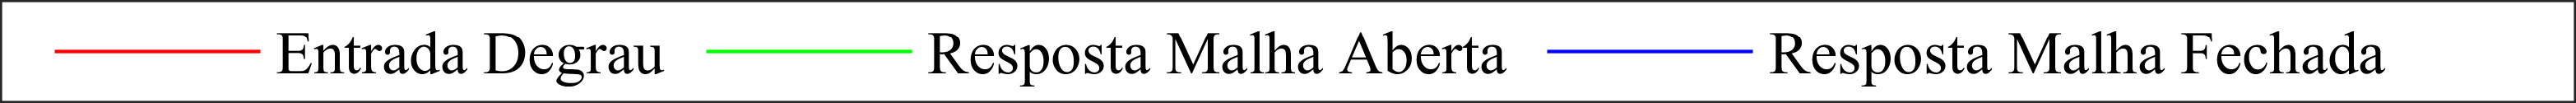
\includegraphics[width=7cm]{img/sim_linear_simulink_temp_leg.png}
            \caption{Simulação da resposta temporal com o controlador projetado na subseção \ref{sc:projeto_controlador_full} para o sistema linearizado em malha aberta e malha fechada.Estados $V_c = \ddot{x}_c$ e $V_w = \ddot{x}_w$ }
            \label{fig:simulaca_temporal_linear_perturbacao}
        \end{centering}
    \end{figure}
    \FloatBarrier
Para a análise da resposta dinâmica do sistema controlado permanecem válidas as mesmas considerações apresentadas na seção \ref{sc:analise_resposta}

\subsection{Projeto de um controlador baseado no observador para o sistema linearizado considerando
que apenas algumas variáveis de estado não são mensuráveis}

Considerou-se para efeitos práticos que as variáveis de estado $x_w$ e $\dot{x}_w$, correspondentes a posição vertical do eixo da roda e sua respectiva velocidade, não são mensuráveis.

Foi decidido que a dinâmica do estimador de estados deve ser 3 vezes  mais rápida do que a dinâmica do sistema linearizado, cujos autovalores são exibidos em \ref{eq:autovalores}. Foi adicionado um valor de offset aos autovalores da planta original, os autovalores resultantes para a dinâmica do preditor linear são exibidos a seguir:

 \begin{equation} \label{eq:autovalores_pred}
        \begin{split}
              \mathbf{eig(A-L*C)}=\
        \end{split}
        \begin{bmatrix}
             -36.0016& +72.3231i&\\
             -36.0016& -72.3231i&\\
             -27.9577& +47.1507i&\\
             -27.9577& -47.1507i&\\
        \end{bmatrix}
    \end{equation}

Na figura a seguir é demonstrado como ficou o design de todos os autovalores do projeto.

    \FloatBarrier
    \begin{figure}[htbp]
        \begin{centering}
            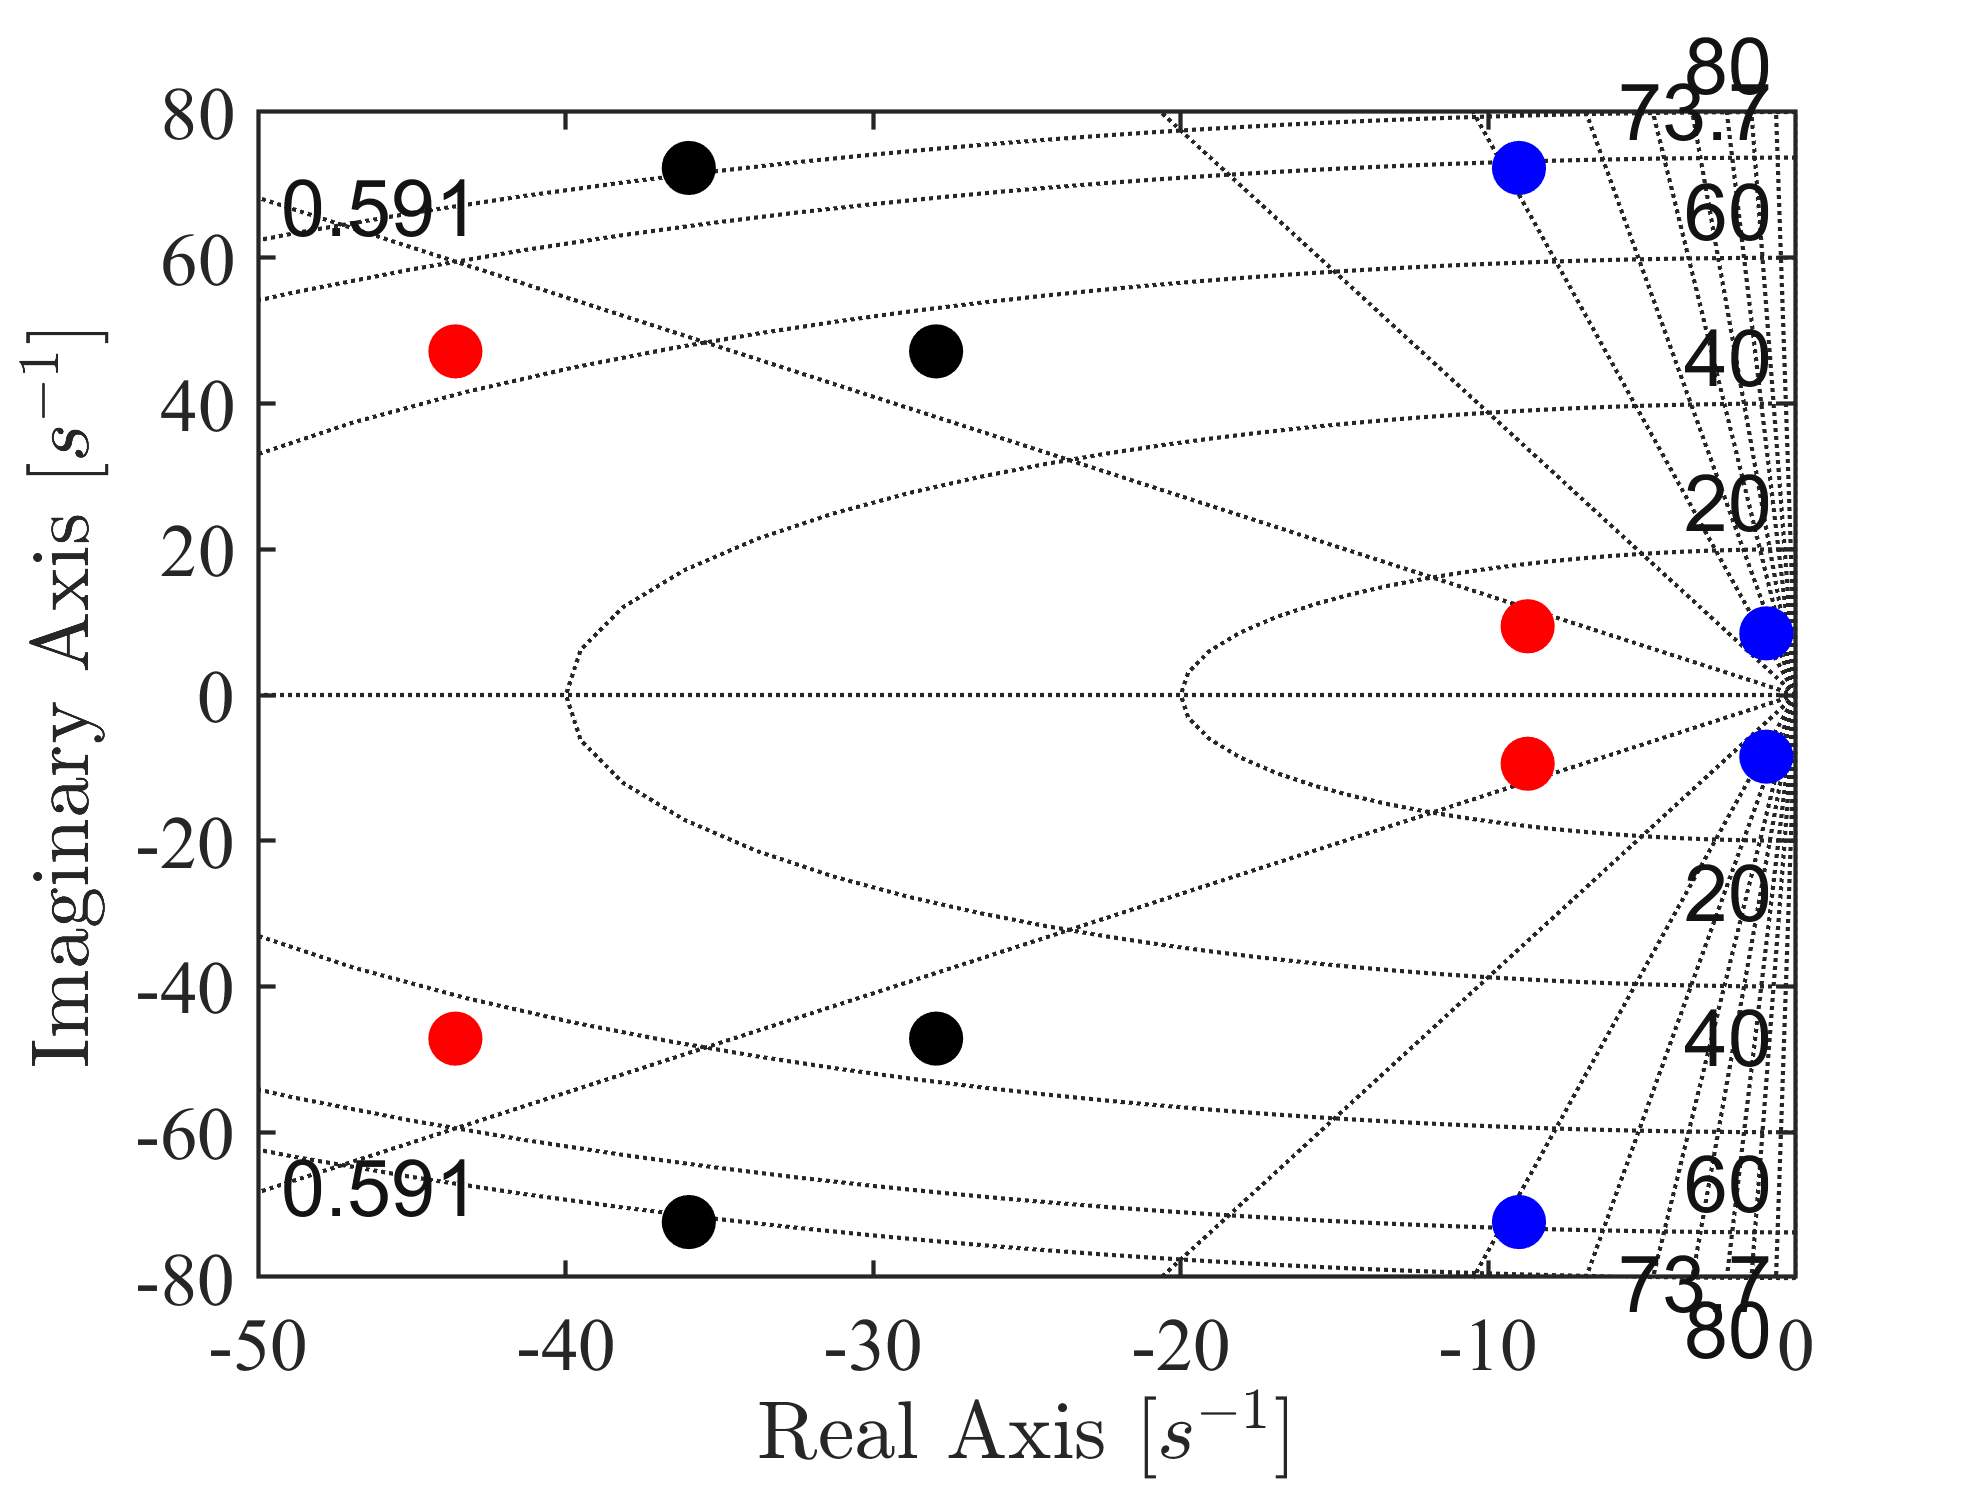
\includegraphics[width=6cm]{img/autovalores_projeto.png}
            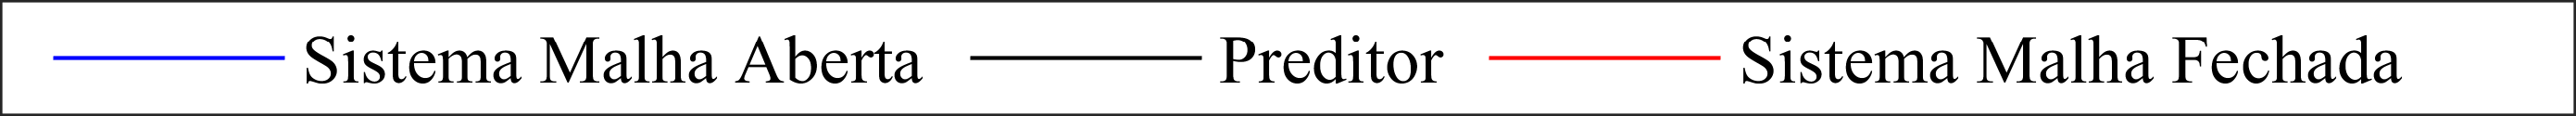
\includegraphics[width=5cm]{img/autovalores_projeto_leg.png}
            \caption{Simulação do erro dos estados entre o sistema original e o preditor lineares em malha fechada.}
            \label{fig:autovalores_projeto}
        \end{centering}
    \end{figure}
    \FloatBarrier
    

Os autovalores foram utilizados para definir o conjunto de ganhos $L$ do observador de estados através da fórmula de Lyapunov definida em \ref{eq:lyapunov}. No entanto empregou-se a seguinte substituição de variáveis:
 \begin{equation} \label{eq:var_pred}
        \begin{split}
        A = A^{t}&\\
        B = C^{t}&
        \end{split}
 \end{equation}

Desta maneira, foi encontrada a seguinte matriz de ganhos de realimentação para o observador de estados linear, números arredondados na quarta casa decimal:

 \begin{equation} \label{eq:ganhos_pred}
        \begin{split}
            \mathbf{L}=\
        \end{split}
        \begin{bmatrix}
          -49.2677& -49.2677& -49.2677& -49.2677&\\
          157.2726& 157.2726& 157.2726& 157.2726&\\
            6.0681&   6.0681&   6.0681&   6.0681&\\
          715.2966& 715.2966& 715.2966& 715.2966&\\
        \end{bmatrix}
    \end{equation}

    Uma simulação temporal do sistema não linear controlado pelo ganho de realimentação de estados, obtido através do preditor desenvolvido nesta seção é exibido nas figuras abaixo:

    \FloatBarrier
    \begin{figure}[htbp]
        \begin{centering}
            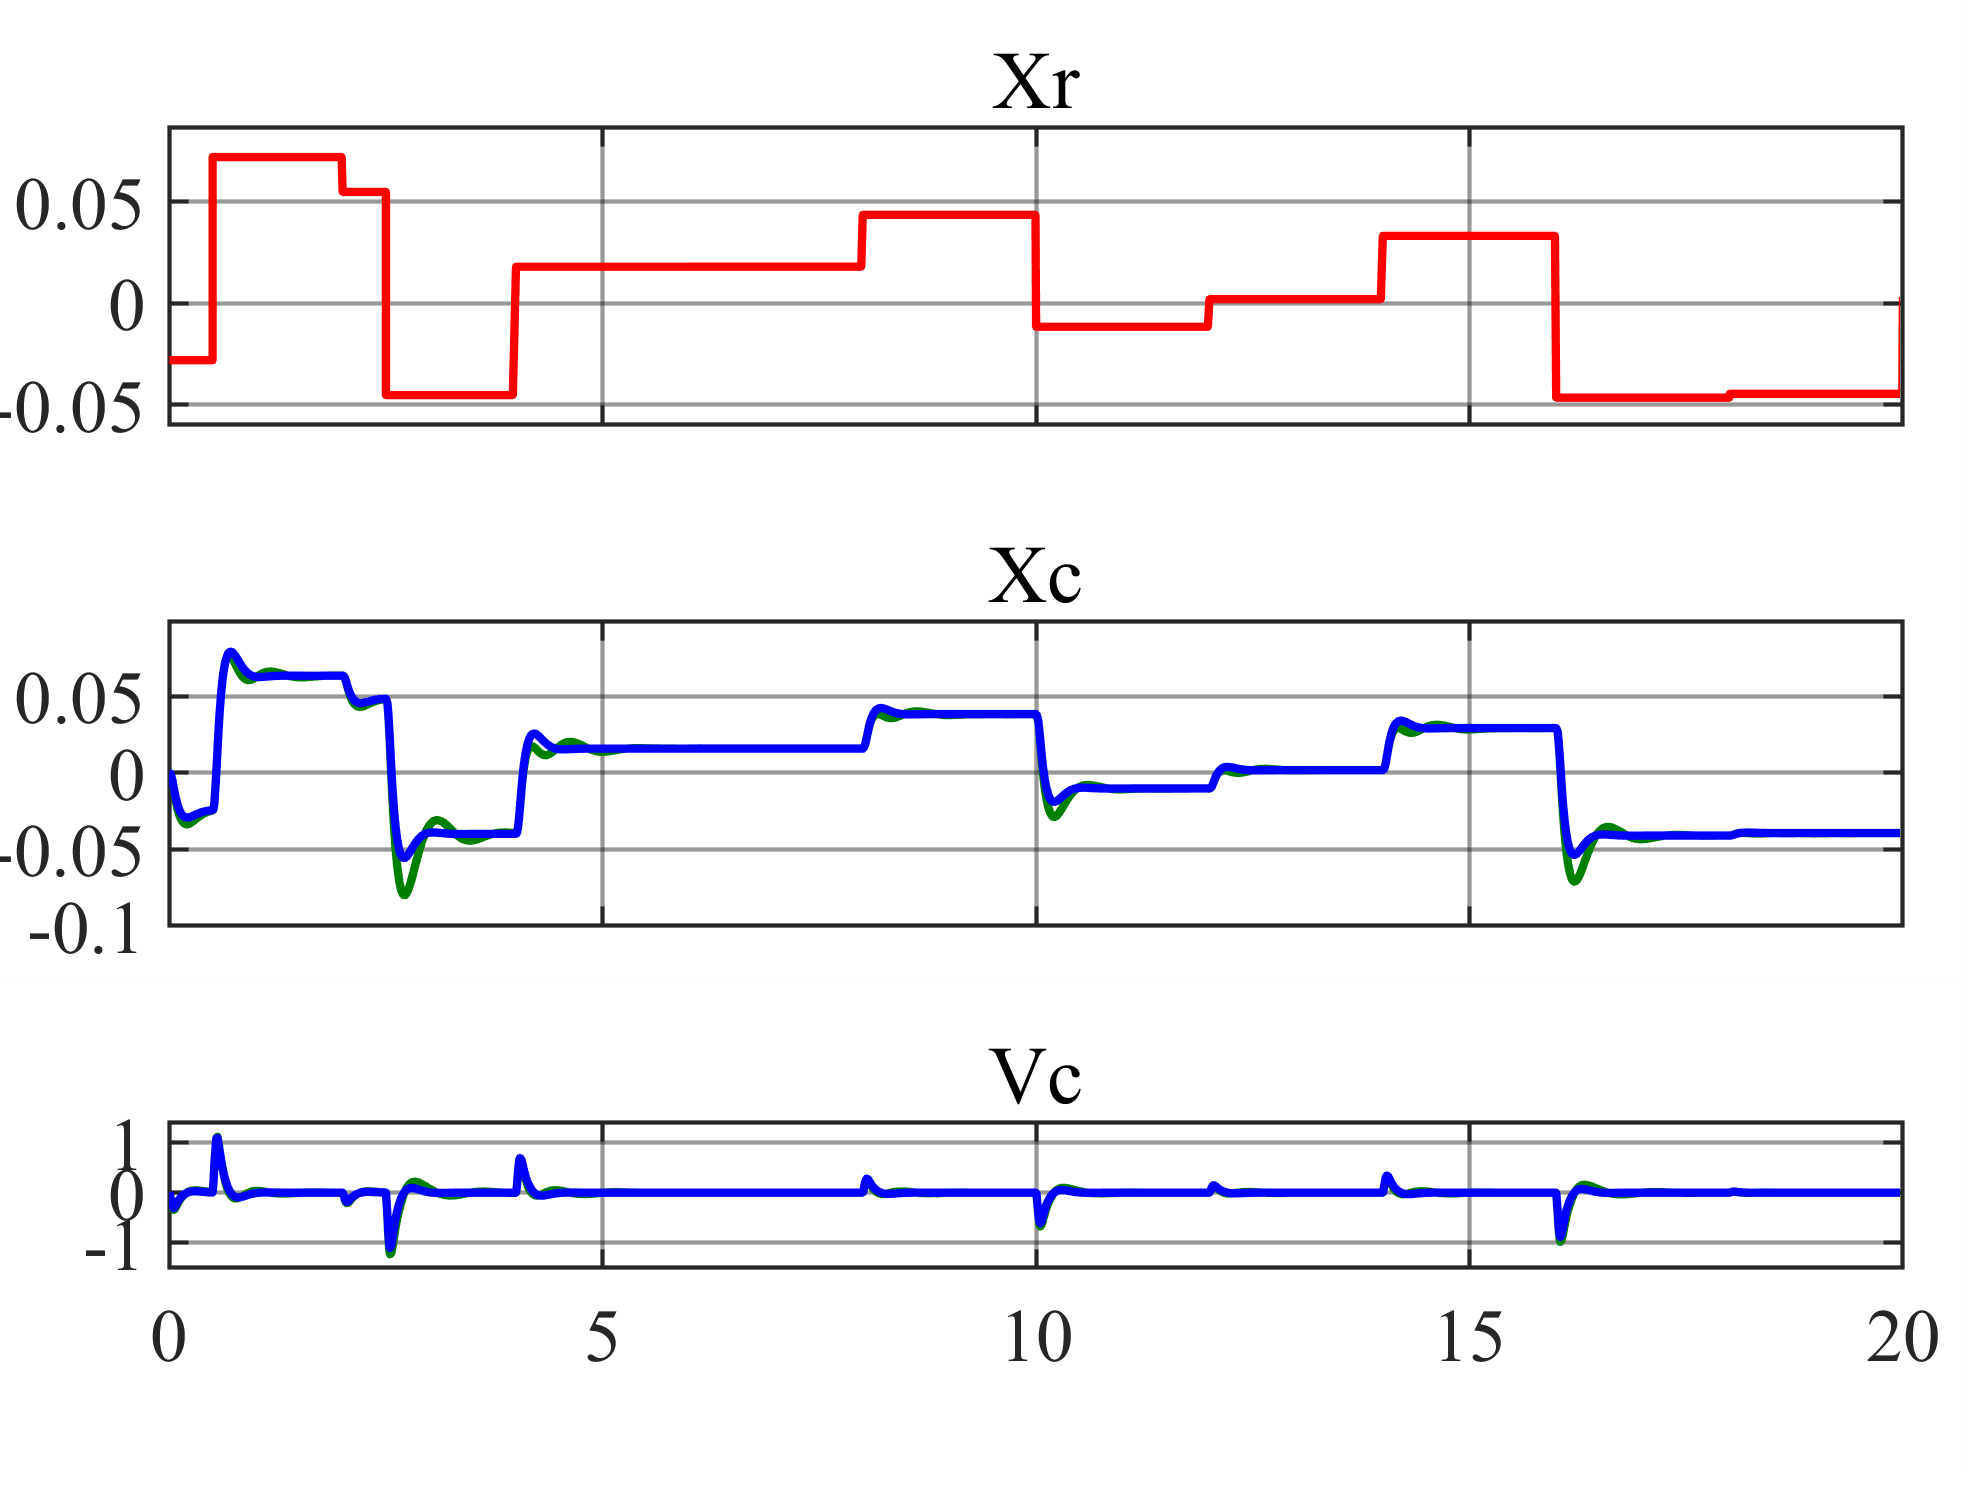
\includegraphics[width=8cm]{img/simulaca_temporal_preditor_linear.png}
            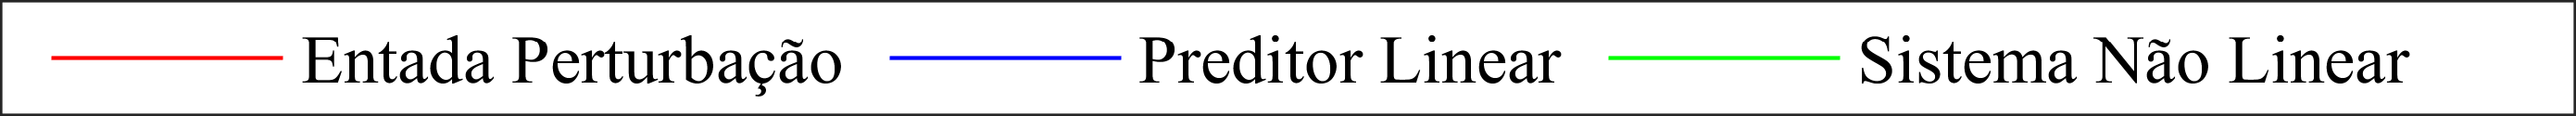
\includegraphics[width=7cm]{img/simulaca_temporal_preditor_linear_erro_leg.png}
            \caption{Simulação da resposta temporal do sistema original com o controlador e o preditor lineares em malha fechada.}
            \label{fig:simulaca_temporal_linear_perturbacao}
        \end{centering}
    \end{figure}
    \FloatBarrier

    \FloatBarrier
    \begin{figure}[htbp]
        \begin{centering}
            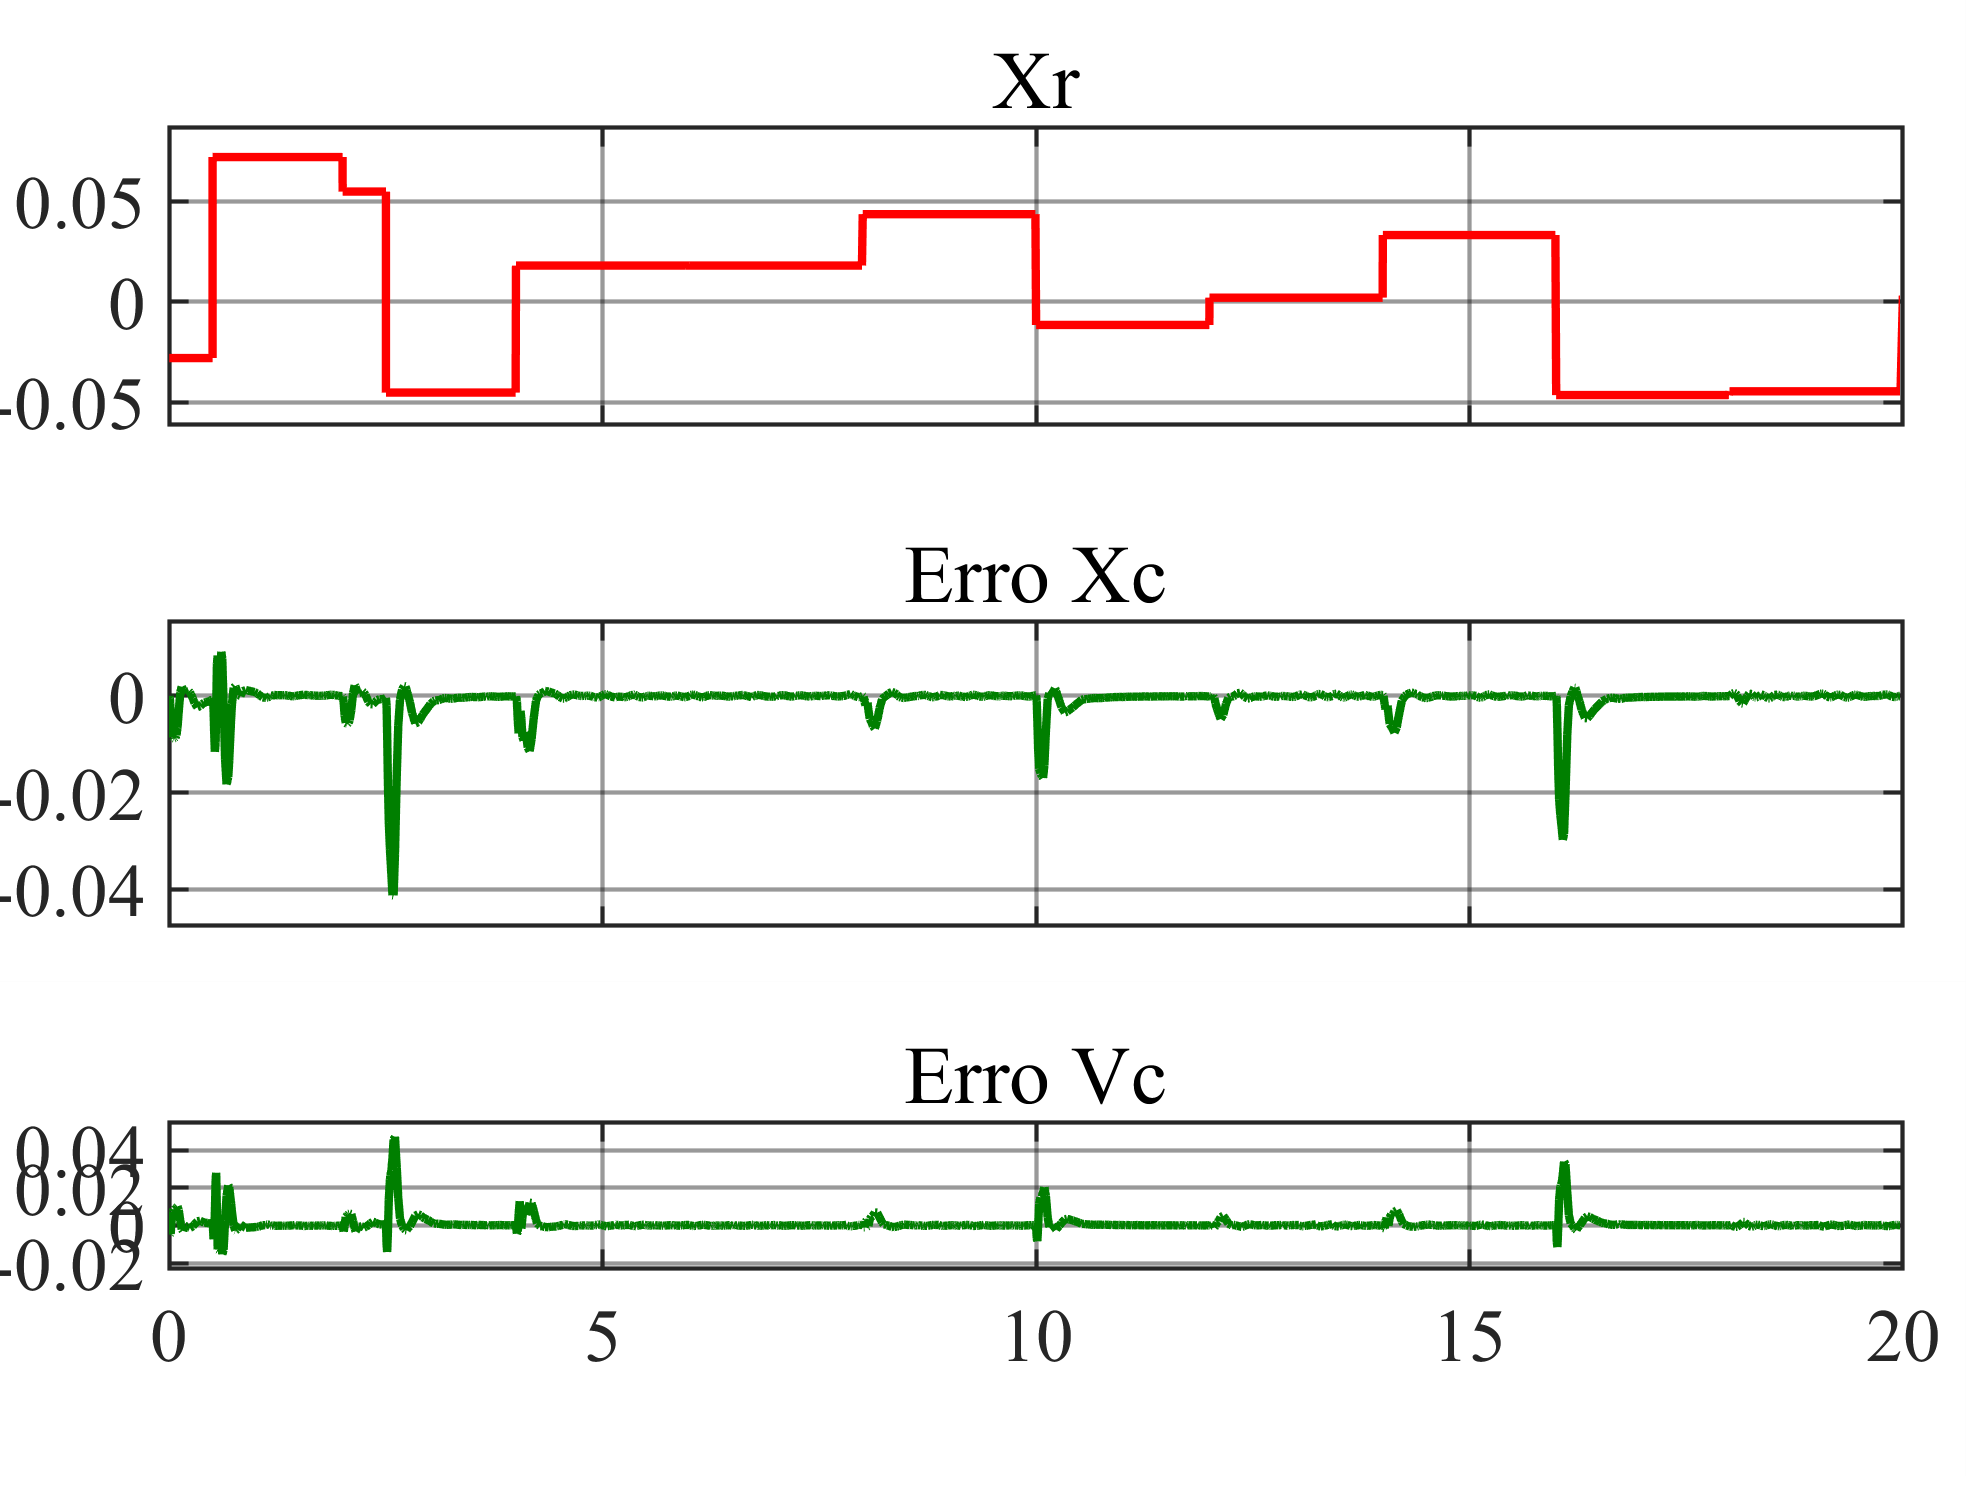
\includegraphics[width=8cm]{img/simulaca_temporal_preditor_linear_erro.png}
            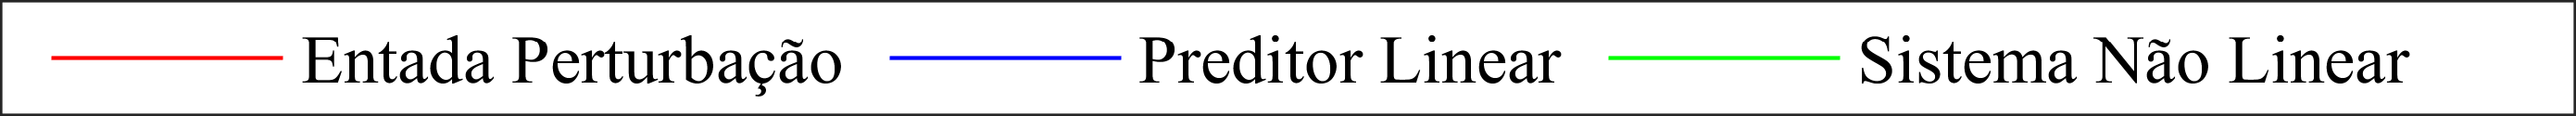
\includegraphics[width=7cm]{img/simulaca_temporal_preditor_linear_erro_leg.png}
            \caption{Simulação do erro dos estados entre o sistema original e o preditor lineares em malha fechada.}
            \label{fig:simulaca_temporal_linear_perturbacao}
        \end{centering}
    \end{figure}
    \FloatBarrier

    O desempenho do sistema real controlado em malha fechada com restrição dos estados observáveis ficou um pouco pior quando comparado com a situação onde todos os estados são observáveis. Especialmente durante os transitórios da perturbação. No entanto, para pequenas variações, o controle baseado em realimentação de estados de um observador linear se mostrou satisfatório.

    \section{Resultados}
    \section{Conclusão}
    
    \bibliography{references,manual}
    
    \appendix
    \section{Lista de siglas e abreviações}
    \begin{itemize} 
        \item [$m_s$] Massa suspensa.
        \item [$m_u$] Massa não suspensa.
        \item [$b_s$] Coeficiente de amortecimento do amortecedor passivo. 
        \item [$k_s$] Coeficiente de elasticidade do feixe de molas da suspensão.
        \item [$k_t$] Coeficiente de elasticidade do pneu.
        \item [$x_r$] Deslocamento vertical da pista.
        \item [$x_w$] Deslocamento vertical da roda.
        \item [$x_c$] Deslocamento vertical da carroceria.
        \item [$F$] Força aplicada pelo amortecedor ativo ou semi-ativo.
        \item [$k^{l}_{s}$] Coeficiente de elasticidade do termo linear no modelo não linear do feixe de molas da suspensão.
        \item [$k^{nl}_{s}$] Coeficiente de elasticidade do termo não linear no modelo não linear do feixe de molas da suspensão.
        \item [$b^{l}_{s}$] Coeficiente de amortecimento do termo da faixa de operação linear do amortecedor.
        \item [$b^{l}_{s}$] Coeficiente de amortecimento do termo da faixa de operação não linear do amortecedor.
        \item [$b^{y}_{s}$] Coeficiente que representa a característica  de comportamento assimétrico do amortecedor.
    \end{itemize}
    
\end{document}